\documentclass[12pt, a4paper]{scrartcl}

% CONFIG
\newcommand{\exptitle}{Halbleiter}       % long name of experiment 
\newcommand{\exptitleshort}{Halbleiter} % short name of experiment
\newcommand{\expdate}{2. und 6. Oktober, 2014}           % date of experiment
\newcommand{\exptutor}{Marc \textsc{Hauser}}

% PACKAGES + MODIFICATIONS
\usepackage[ngerman]{babel} %standard language stuff
\usepackage[T1]{fontenc}
\usepackage[utf8]{inputenc}

\usepackage[fleqn]{amsmath}  % math
\usepackage{amssymb}

\usepackage{graphicx} %graphics
\usepackage{float} 

\usepackage{textgreek}

\usepackage[automark,headsepline]{scrlayer-scrpage} %headings
\pagestyle{scrheadings}
\ihead{\exptitleshort}
\ohead{\pagemark}
\cfoot{}

\usepackage{hyperref}
\hypersetup{
    unicode=true,          % non-Latin characters in Acrobat’s bookmarks
    pdftoolbar=true,       % show Acrobat’s toolbar?
    pdfmenubar=true,       % show Acrobat’s menu?
    pdffitwindow=false,    % window fit to page when opened
    pdfstartview={FitH},   % fits the width of the page to the window
    pdfnewwindow=true,     % links in new window
    colorlinks=true,       % false: boxed links; true: colored links
    linkcolor=blue,       % color of internal links (change box color with linkbordercolor)
    citecolor=green,       % color of links to bibliography
    filecolor=magenta,     % color of file links
    urlcolor=blue          % color of external links
}

\usepackage[labelfont=bf]{caption} % bold captions

\usepackage{chngcntr} % change behaviour of counters in different environments
\counterwithin{figure}{section}  % number figures per section
\numberwithin{equation}{section} % number equations per section
\numberwithin{table}{section}    % number tables per section

\usepackage{enumerate} % better way to config enumerates

\setcounter{tocdepth}{2} % table of contents depth

\setlength{\parindent}{0pt} % no indent on new paragraph

\usepackage{pdfpages} % include pdf files

% NEW COMMANDS
\newcommand{\difd}{\mathrm{d}}

% DOCUMENT SETTINGS

\title{\exptitle}
\subtitle{Fortgeschrittenen-Praktikum 1}
\author{Moritz Bitterling und Benjamin Rottler \\ Universität Freiburg}
\date{\expdate}

% DOCUMENT
\begin{document}

\hypersetup{pageanchor=false} %stop page numbering (hyperref) to prevent for double page numers
\newcommand{\HRule}{\rule{\linewidth}{0.5mm}}
\begin{titlepage}
\begin{center}
  \textsc{\Large Fortgeschrittenen-Praktikum I}\\[0.5cm]
  \HRule \\[0.4cm]
  { \huge \bfseries \exptitle}\\
  \HRule \\[0.5cm]
  \large \expdate\\[0.5cm]  
  \begin{minipage}{0.4\textwidth}
    \begin{flushleft} \large
      Moritz \\ \textsc{Bitterling}
    \end{flushleft}
  \end{minipage}
  \hfill
  \begin{minipage}{0.4\textwidth}
    \begin{flushright} \large
      Benjamin \\ \textsc{Rottler}
    \end{flushright}
  \end{minipage}
  \\[1cm]
  \large 
  Betreuer: Riccardo \textsc{Mori} \\[3cm]
  
\includegraphics[height=8cm]{../../img/logo_uni.pdf}
  \vfill
  \normalsize
  \textsc{Institut für Mathematik und Physik} \\
  \textsc{Albert-Ludwigs-Universität} \\
  \textsc{Freiburg im Breisgau}
\end{center}
\end{titlepage}
\thispagestyle{empty}

\newpage
Alle Berechnungen in diesem Protokoll wurden unter Python 2.7 mit Hilfe folgender Programmbibliotheken
\begin{itemize}
  \item PyROOT (\url{http://root.cern.ch/drupal/content/pyroot})
  \item NumPy (\url{http://www.numpy.org/})
\end{itemize}
oder mit Mathematica 10 durchgeführt. \\
Die Graphiken wurden mit Inkscape (\url{http://www.inkscape.org}) gezeichnet.\\[\baselineskip]
Alle Python-Skripte, \LaTeX-Skripte und SVG-Graphiken können online unter \\
\url{https://github.com/Bigben37/FP1/tree/master/0908-LHWZ} abgerufen werden.
\thispagestyle{empty}

\newpage
\tableofcontents
\thispagestyle{empty}

\newpage
\hypersetup{pageanchor=true} %start page numbering again
\setcounter{page}{1} %set to page 1

Kurze Beschreibung des Versuchs und Nennung wesentlicher Ziele.
\section{Physikalische Grundlagen}
Die Gleichungen und Erklärungen dieses Kapitels beruhen auf \cite{herrmann}.
\subsection{Teil I: Pockels-Effekt}

\subsubsection{Elektrooptischer Effekt}
Die elektrische Flussdichte $D$ ändert sich, wenn man ein äußeres elektrisches Feld anlegt. Diese Veränderung wird 
\emph{elektrooptischer Effekt} genannt und durch folgende Formel beschrieben:
\begin{equation}
\label{eq:eoeff}
  D = a \cdot E + b \cdot E^2 + c \cdot E^3 + \ldots
\end{equation}
Die Dielektrizitätskonstante\footnote{Wie man hier sieht, ist die Dielektrizitätskonstante keine Konstante, der Name hat historischen Ursprung.} 
$\epsilon$ lässt sich durch Differentiation von $D$ nach $E$ berechnen.
\begin{equation}
\label{eq:dielconst}
  \epsilon = \frac{\difd D}{\difd E} = a + 2 \cdot b \cdot E + 3 \cdot c \cdot E^2 + \ldots
\end{equation}
Der lineare elektrooptische Effekt oder \emph{Pockels-Effekt} tritt bei Kristallen ohne Symmetriezentrum auf, was zur Folge hat, dass 
der lineare Teil $2 \cdot b \cdot E$ nicht verschwindet. Der Einfluss von höheren Potenzen von $E$ ist sehr gering, da die Konstanten 
$b, c, \ldots$ sehr kleine Werte annehmen, und kommt nur bei sehr hohen elektrischen Feldstärken zum tragen. 
Für $b = 0$ und $c \neq 0$ spricht man vom \emph{Kerr-Effekt}. \\
Da der Brechungsindex $n$ von der Dielektrizitätskonstante abhängt, wirkt sich der Po"-ckels-Effekt auf die Brecheigenschaften des Kristalls aus.
\begin{equation}
  n = \sqrt{\epsilon \mu}
\end{equation}

\subsubsection{Doppelbrechung in Kristallen}
In einem optisch isotropen Medium ist die Lichtausbreitung unabhängig von der Ausbreitungsrichtung und Polarisation des Lichtes. Dies gilt bei 
einem optisch anisotropen Medium nicht mehr, man spricht von \emph{Doppelbrechung}. Bei optisch anisotropen Medien unterscheidet man zwischen 
optisch einachsigen und optisch zweiachsigen. Ja nach Typ gibt es eine oder zwei ausgezeichnete Richtungen, in denen ein Lichtstrahl für alle 
Polarisationen die gleiche Ausbreitungsgeschwindigkeit besitzt. \\
Man führt die Bezeichnung ordentlicher und außerordentlicher Strahl ein. Der ordentliche Strahl ist die Komponente des $E$-Feldes, die senkrecht 
auf dem Hauptschnitt (Ebene, die durch den $\vec{k}$-Vektor und die optische Achse des Kristalls aufgespannt wird) steht. Der außerordentliche 
Strahl liegt in der Ebene des Hauptschnitts.\\
Der Formalismus des Brechungsindex-Ellipsoids ist eine einfache Möglichkeit zur Beschreibung der Doppelbrechung. 
\begin{equation}
  \frac{x_1^2}{n_1^2 } +\frac{x_2^2}{n_2^2 } +\frac{x_3^2}{n_3^2 } = 1 
\end{equation}
Die Koordinaten $x_1, x_2, x_3$ spannen ein kartesisches Koordinatensystem auf. Mindestens eine Achse muss parallel zu einer kristallographischen 
Achse des Kristalls liegen. Die Brechungsindizes $n_1, n_2, n_3$ gelten für Licht, das sich parallel zu den entsprechenden Achsen ausbreitet. 
Kennt man das Brechungsindex-Ellipsoid, so kann man die unterschiedlichen Ausbreitungsrichtungen mit 
$v=\frac{c}{n}$ bestimmen. Die Form des Brechungsindex-Ellipsoid eines optisch isotropen Mediums ist eine Kugel, es verformt sich zu einer 
Ellipse bei einem anisotropen Medium.

\subsubsection{Konfiguration der Pockelszelle}
\paragraph{Bestimmung der Brechungsindizes}
In diesem Versuch wird eine Pockelszelle, die aus vier ADP\footnote{Ammoniumdihydrogenphosphat}-Kristallen mit einem $45^\circ Y$-Cut besteht, 
verwendet. Legt man an eine normale ADP-Zelle einen Spannung $E_1$ entlang der $x_1$ Achse an, so lautet das Indexellipsoid nach \cite{manual}:
\begin{equation}
  \frac{x_1^2}{n_1^2} + 2 \cdot r_{41} \cdot E_1 \cdot x_3 + \frac{x_2^2}{n_1^2} + \frac{x_3^2}{n_3^2} = 1
\end{equation}
mit $r_{41}$ als \emph{elektrooptischer Koeffizient}. Man erkennt, dass der Kristall optisch einachsig ist und die $x_3$-Achse die optische Achse ist. \\
Der $45^\circ Y$-Cut wird mit Hilfe einer Koordinatentransformation berücksichtigt:
\begin{equation}
  x_2 = \frac{1}{\sqrt{2}} \left( x_2' + x_3' \right), \qquad x_3 = \frac{1}{\sqrt{2}}(x_2' - x_3')
\end{equation}
Daraus folgt nach \cite{manual} für den Brechungsindex der $x_2'$-Achse:
\begin{equation}
  \label{eq:refindex:x2new}
  n_{x_2'} \approx n_x + \frac{1}{2} \cdot r_{41} \cdot E_1 \cdot n_x^3
\end{equation}
mit
\begin{equation}
  \label{eq:nxdef}
  \frac{1}{n_x^2} = \frac{1}{2} \left( \frac{1}{n_2^2} + \frac{1}{n_3^2} \right)
\end{equation}
\paragraph{Bestimmung der Phasenverschiebung}
Die ortsabhängige Amplitude des sich im Kristall ausbreitenden Lichts lässt sich mit
\begin{equation}
  A(x) = A_0 \cdot e^{ikx} = A_0 \cdot e^{i \varphi(x)}
\end{equation}
beschreiben. Mit der \emph{Dispersionsrelation} $\omega = v\cdot k$ und den Beziehungen $\omega = 2 \pi f$, $c = f \cdot \lambda$ 
und $v = \frac{c}{n}$ folgt für die Phase $\varphi$ der Welle.
\begin{equation}
  \varphi(x) = \frac{2 \pi}{\lambda} \cdot n \cdot x
\end{equation}
Es ergibt sich eine Phasendifferenz $\Delta \varphi$ in einem Kristall der Länge $l$ von
\begin{equation}
  \Delta \varphi = \frac{2 \pi}{\lambda} \cdot l \cdot \left( n_1 - n_{x_2'} \right) 
\end{equation}
Durch die Lage der optischen Achse laufen jetzt jedoch ordentlicher und außerordentlicher Strahl auseinander. Sie werden mit einem zweiten, 
um $180^\circ$ gedrehten ADP-Kristall wieder zusammengeführt. Die Phasendifferenz verdoppelt sich.
\begin{equation}
  \Delta \varphi = \frac{4 \pi}{\lambda} \cdot l \cdot \left( n_1 - n_{x_2'} \right) 
\end{equation}
Da der ADP-Kristall ein optisch einachsiger Kristall ist, besitzt er auch natürliche Doppelbrechung $n_1 - n_x$. Diese wird durch ein zweites 
Kristallpaar, das um $90^\circ$ gedreht ist ausgeglichen. Um Pockels-Effekt nicht auch aufzuheben, wird das zweite Paar mit invertierter Spannung 
betrieben. Dadurch verdoppelt sich die Phasendifferenz noch einmal. Es gilt also:
\begin{equation}
  \begin{split}
    \Delta \varphi &= \frac{8 \pi}{\lambda} \cdot l \cdot \left( n_1 - n_{x_2'} \right) \\
    &\refeq{eq:refindex:x2new} \frac{8 \pi}{\lambda} \cdot l \cdot \left( \underbrace{n_1 - n_x}_{=0} + \frac{1}{2} \cdot r_{41} \cdot E_1 \cdot n_x^3 \right) \\
    & = \frac{4 \pi}{\lambda} \cdot l \cdot r_{41} \cdot E_1 \cdot n_x^3  
  \end{split}
\end{equation}
Legt man nun die Halbwellenspannung $U_{\lambda/2}$ an, so beträgt die Phasendifferen gerade $\Delta \varphi = \pi$.
Unter Verwendung von $E=\frac{U_{\lambda/2}}{d}$ und \autoref{eq:nxdef} lässt sich der \emph{elektrooptische Koeffizient} $r_{41}$ folgendermaßen bestimmen:
\begin{equation}
  \label{eq:r41}
  r_{41} = \frac{\lambda \cdot d}{4 \cdot l \cdot U_{\lambda/2}} \sqrt{\frac{1}{2} \left( \frac{1}{n_1^2} + \frac{1}{n_3^2} \right) }^3
\end{equation}
mit $l$ Länge und $d$ Dicke (Kantenlänge) der Pockelszelle, sowie der Brechungsindizes $n_1$ und $n_3$.

\subsection{Teil II: Faraday-Effekt}
\subsubsection{Faraday-Effekt}
Der \emph{Faraday-Effekt} tritt auf, wenn linear polarisiertes Licht durch ein isotropes Medium, welches mit ein Magnetfeld in 
Ausbreitungsrichtung des Lichts durchflossen ist, propagiert. Das Magnetfeld verursacht eine zirkulare Doppelbrechung, das heißt links- und 
rechtsdrehende elektromagnetische Wellen haben einen unterschiedlichen Brechungsindex. \\
Da linear polarisiertes Licht als Überlagerung von zwei, in entgegengesetzter Richtung zirkular polarisierten elektromagnetischen Wellen 
beschrieben werden kann, eilt eine Welle der anderen voraus und das Licht, welches das Medium durchläuft, wird um einen Winkel $\alpha$ gedreht. 
Die Stärke der Drehung hängt proportional von der magnetischen Feldstärke $H$ der Spule ab, welche das Magnetfeld erzeugt. 
Dies bedeutet, dass bei Umkehrung des Spulenstroms, was einer Umpolung entspricht, das Licht in entgegengesetzte Richtung gedreht wird. 
Die Drehung ist also nicht reversibel, spiegelt man das Licht und lässt es das Medium in anderer Richtung durchqueren, 
so verdoppelt sich die Drehung\footnote{Im Gegensatz zu optisch aktiven Substanzen, die eine ausgezeichnete Drehrichtung haben 
und die erste Drehung rückgängig machen.}. Weiterhin hängt der Drehwinkel $\alpha$ proportional von der Länge $l$ des Mediums ab.
Es gilt also:
\begin{equation}
\label{eq:faraday}
  \alpha = V \cdot l \cdot H
\end{equation}
wobei $V$ eine Materialkonstante, auch \emph{Verdet-Konstante} genannt, ist.

\subsubsection{Bestimmung der magnetischen Feldstärke einer Zylinderspule}
\paragraph{Gesetz von Biot-Savart}
Die magnetische Flussdichte $\difd \vec{B}$ am Ort $\vec{r}$ eines mit dem Strom $I$ durchflossenen Leiters mit Länge $\difd \vec{l}$ 
am Ort $\vec{r}'$ lässt sich mit Hilfe des \emph{Biot-Savart}-Gesetzes bestimmen:
\begin{equation}
  \label{eq:biotsavart}
  \difd \vec{B}(\vec{r}) = \frac{\mu_0 \cdot I}{4 \pi} \cdot \difd \vec{l} \times \frac{\vec{r} - \vec{r}'}{\abs{\vec{r} - \vec{r}'}^3}
\end{equation}
\paragraph{Kreisförmige Leiterschleife}
Es wird zuerst eine kreisförmige Leiterschleife parallel zu der $x$-$y$-Ebene mit dem Radius $R$ betrachtet (\autoref{img:circloop}) \cite{dem2}. %TODO Skizze
Da die Komponente $\difd B_\perp = \difd B \cdot \sin \alpha$ senkrecht zur $z-$Achse bei der Integration über $\difd l$ verschwindet 
(Rotationssymmetrie), bleibt es nur die parallele Komponente $\difd B_\parallel = \difd B \cdot \cos \alpha$ zu betrachten. Wie in 
\autoref{img:bvector} zu erkennen ist, gilt
\begin{equation}
\label{eq:absdif}
  \abs{\difd \vec{l} \times \left( \vec{r} - \vec{r}' \right)} = \abs{\vec{r} - \vec{r}'} \cdot \difd l \cdot \underbrace{\sin \varphi}_{= 1} 
  = \abs{\vec{r} - \vec{r}'} \cdot \difd l = \frac{R}{\cos \alpha} \cdot \difd l
\end{equation}
Es folgt für $B_\parallel$:
\begin{equation}
\begin{split}
  \label{eq:bparallel}
    B_\parallel &= \int \difd B_\parallel = \int \difd B \cdot \cos \alpha \\
  &\refeq{eq:faraday} \frac{\mu_0 \cdot I}{4 \pi} \cdot \oint \frac{\abs{\difd \vec{l} \times \left( \vec{r} - \vec{r}' \right)}}{\abs{\vec{r} - \vec{r}'}^3} \cdot \cos \alpha \\
  &\refeq{eq:absdif} \frac{\mu_0 \cdot I}{4 \pi} \cdot \frac{R}{\abs{\vec{r} - \vec{r}'}^3} \cdot \oint \difd s = \frac{\mu_0 \cdot I}{2} \cdot \frac{R^2}{\abs{\vec{r} - \vec{r}'}^3}
\end{split}
\end{equation}
Mit $\abs{\vec{r} - \vec{r}'}^2 = R^2 + (z-z')^2$ folgt damit für die magnetische Flussdichte $\vec{B}_K(z, z')$
\begin{equation}
  \vec{B}_K(z, z') = B_\parallel \cdot \hat{e}_z \refeq{eq:bparallel} \frac{\mu_0 \cdot I}{2} \cdot \frac{R^2}{ \left( R^2 + (z-z')^2 \right)^{3/2}} \cdot \hat{e}_z
\end{equation}
Die magnetische Feldstärke $H_K$ ist also
\begin{equation}
  H_K(z, z') = \frac{B_K(z, z')}{\mu_0} = \frac{I}{2} \cdot \frac{R^2}{ \left( R^2 + (z-z')^2 \right)^{3/2}}
\end{equation}
\paragraph{Reale Zylinderspule}
Eine reale Zylinderspule der Länge $L$ besitzt einen Innen- und Außenradius ($r_i$ und $r_a$). 
Weiterhin wird angenommen, dass die Windungen $N$ homogen gewickelt sind. Daher gilt für die differentielle Windugszahl $\difd N$ in einem 
Rechteck mit Seiten $\difd z'$ und $\difd R$:
\begin{equation}
  \difd N = \frac{N}{L} \cdot \difd z' \cdot \frac{\difd R}{r_a - r_i}
\end{equation}
Für das Magnetfeld $H(z)$ der realen Spule folgt nun \cite{herrmann}:
\begin{equation}
  \label{eq:hreal}
  \begin{split}
    H(z) &= \frac{N}{L} \cdot \int_{r_i}^{r_a} \frac{\difd R}{r_a - r_i} \cdot \int_{0}^{L} B_K(z, z')\, \difd z'\\
    &=\frac{N \cdot I}{2 L \left( r_a - r_i \right) } \cdot \left[ 
  	      (L-z) \cdot \ln \left( \frac{r_a + \sqrt{(L-z)^2  +r_a^2}}{r_i + \sqrt{(L-z)^2 + r_i^2}} \right) + 
  		  z \cdot \ln \left( \frac{r_a + \sqrt{z^2  +r_a^2}}{r_i + \sqrt{z^2 + r_i^2}} \right)  \right]
  \end{split}
\end{equation}
\subsubsection{Bestimmung des Drehwinkels in Abhängigkeit des Stroms}
\label{subsub:alpha}
Das Licht wird nun nach \autoref{eq:faraday} pro Wegstrecke $\difd z$ um folgenden Winkel $\difd \alpha$ gedreht:
\begin{equation}
  \difd \alpha = V \cdot H(z) \cdot \difd z
\end{equation}
Der gesamte Winkel $\alpha$ berechnet sich mit den gegebenen Werten für diesen Versuch (siehe Kapitel \ref{sub:setup:faraday}) 
zu:\footnote{Mit Mathematica berechnet.}
\begin{equation}
  \label{eq:verdet}
  \alpha = V \int_{\frac{L-l}{2}}^{\frac{L+l}{2}} H(z)\, \difd z = 2554.85 \cdot V \cdot I 
\end{equation}

\section{Vermessung der Bandlücke}
\subsection{Versuchsaufbau}

\subsection{Versuchsdurchführung}

Am Aufbau werden an Germanium und Silizium die gleichen Messungen durchgeführt.
Zu Beginn wird die Nullwinkelstellung des optischen Gitters mit Hilfe des Maximums 0.\,Ordnung gesucht.
Anschließend wird von diesem Maximum ausgehend eine Trans\-missions- und Absorptionsmessung
über den gesamten Winkelbereich durchgeführt.
Außerdem wird mit abgedecktem Halbleiter der Untergrund und ohne Halbleiter das Spektrum der Lampe
mit dem Pyrodetektor vermessen.
Um die Messfehler abzuschätzen, werden an den Maxima von Transmission und Absorption für jeweils 100\,s
halbsekündlich Messwerte aufgenommen.\\
\autoref{tab:einstBL} zeigt die Einstellungen am Lock-in-Verstärker, die für die beiden Messungen verwendet wurden.


\begin{table}[H]
\caption{Einstellungen am Lock-in-Verstärker bei der Bestimmung der Bandlücken.}
\begin{center}
\begin{tabular}{|c|c|c|c|c|c|}
\hline
			&	$I$/mA	&	AC gain pyro	&	AC gain sample	&	DC gain pyro	&	DC gain sample	\\ \hline
Si			&	0.75	&	100				&	10				&	5				&	2				\\ \hline
Ge			&	15.00	&	300				&	1000			&	10				&	5				\\ \hline
\end{tabular}
\end{center}
\label{tab:einstBL}
\end{table}
\subsection{Messergebnisse und Auswertung}
\subsubsection{Bandlückenenergie von Silizium}
Das Spektrum der Absorption (gemessen mit der Silizium-Probe) und Transmission (gemessen mit dem Pyrodetektor) von Silizium 
in Abhängigkeit des Winkels $\alpha$ ist in \autoref{img:si:spectrum} dargestellt. Man erkennt das Maxima 0. Ordnung bei $\alpha = 0^\circ$. 
Durch diese Eichung des Winkels kann das verwendete Messprogramm die Winkel schon in die richtigen Energien 
(abhängig vom Winkel und der Gitterkonstante) umrechnen, welche später noch benötigt werden.
\begin{figure}[H]
\begin{center}
  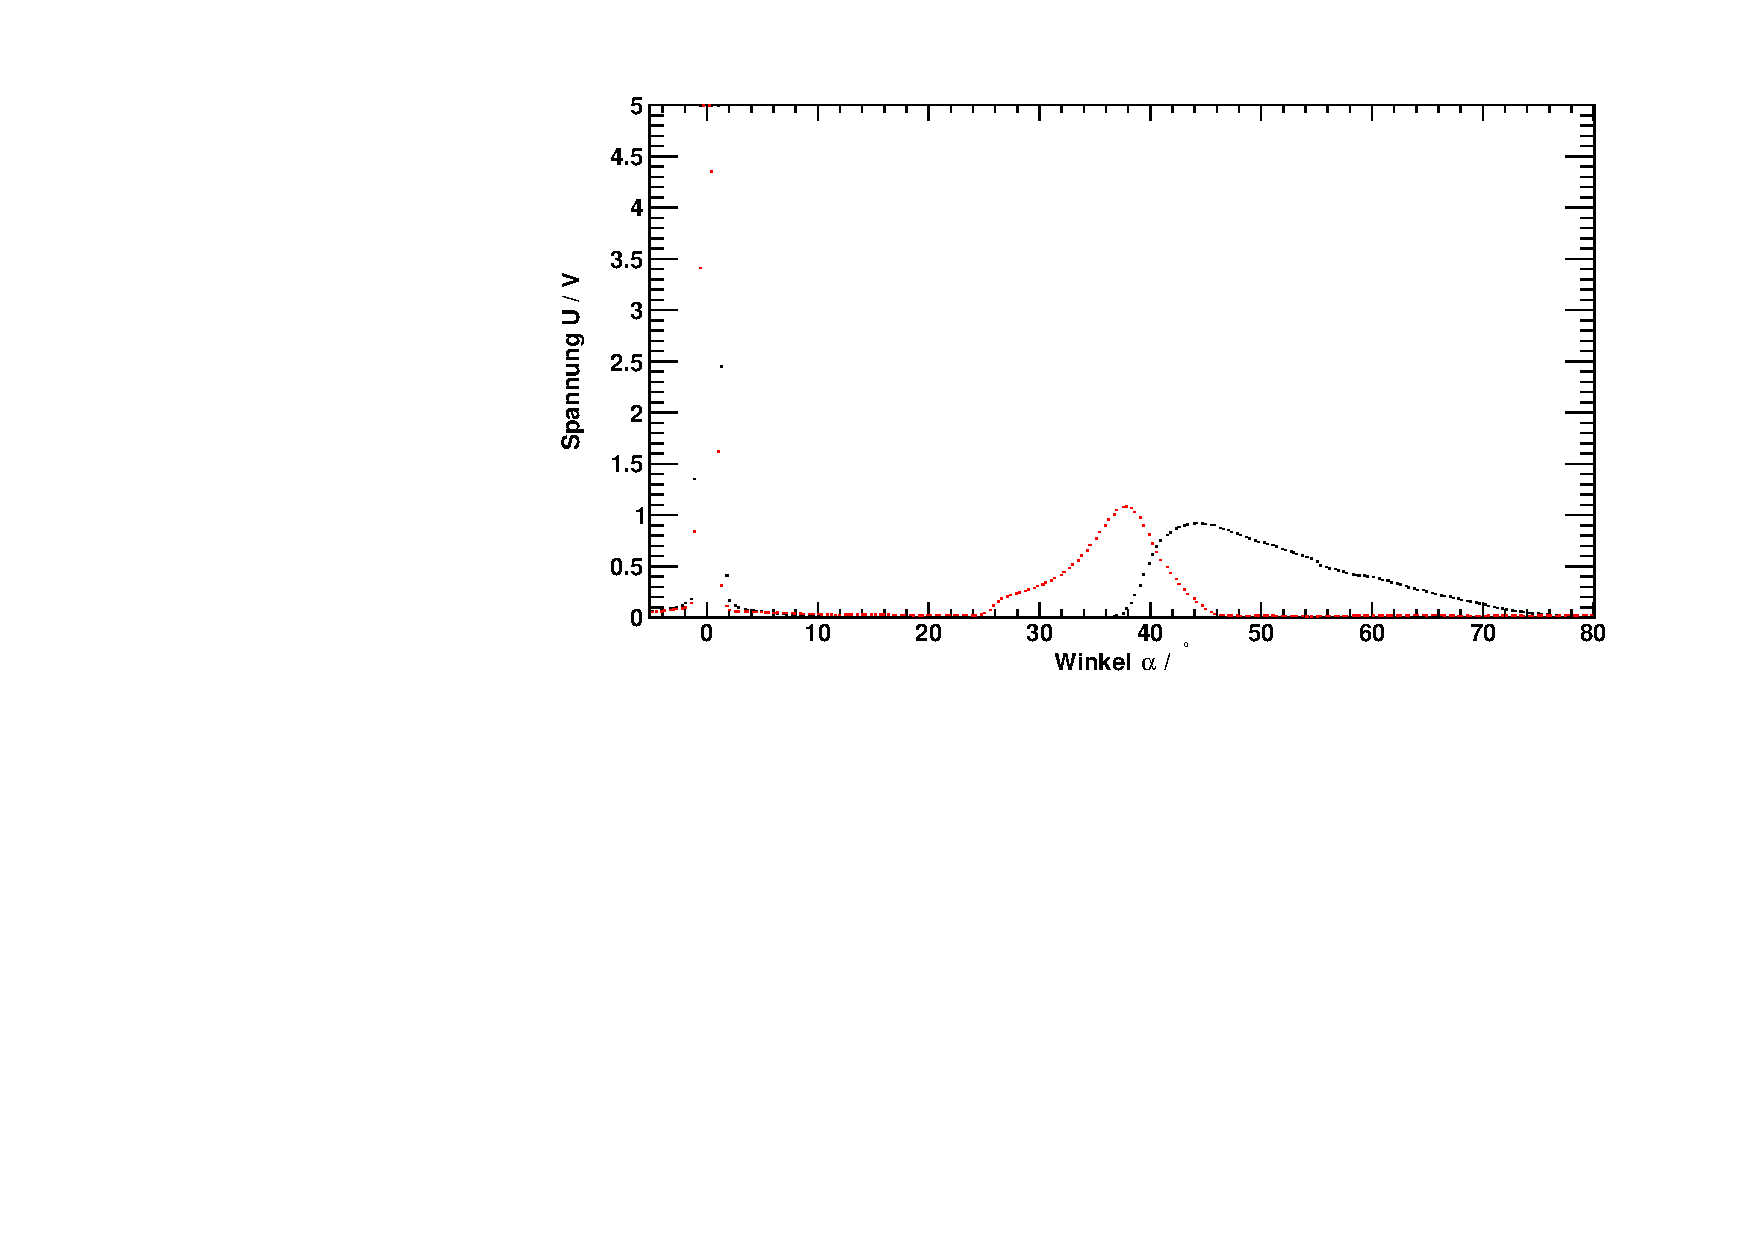
\includegraphics[width=\textwidth]{../img/part1/Si_Messung_spectrum.pdf}
  \caption{Absorptions- und Transmissionsspektrum von Silizium.}
  \label{img:si:spectrum}
\end{center}
\end{figure}

Für die Fehler der Messpunkte wurde die Spannung an den Sensoren über einen längeren Zeitraum ($t=100$\,s) bei den Winkeln der maximalen 
Transmission und Absorption gemessen. Aus dieser Messreihe wurde die Standardabweichung
\begin{equation}
  s_U = \sqrt{ \frac{1}{N - 1} \sum_{i=1}^N \left( \bar{U} - U_i \right)^2 }
\end{equation}
bestimmt und als absoluter Fehler der einzelnen Messpunkte gesetzt.
\begin{equation}
  s_{\text{Abs}} = 0.007\,\text{V}, \qquad s_{\text{Trans}} = 0.004\,\text{V}
\end{equation}

Um die Bandlückenenergie von Silizium zu bestimmen, muss von den beiden Messungen jeweils der Untergrund (\autoref{img:si:underground}) abgezogen 
werden. Des weiteren müssen die Messungen auf die Leistung der Lampe normiert werden, da diese nicht für alle Winkel gleich ist 
(\autoref{img:si:lampe}). Da die Winkel nur jede halbe Sekunde aufgenommen werden, sind die genauen Werte der Winkel nicht reproduzierbar. 
Deshalb wurde für jeden Messpunkt eine lineare Interpolation des Untergrunds und des Spektrums der Lampe zwischen den benachbarten Punkten 
durchgeführt.
\begin{equation}
  I_{\text{Pyro}} = \frac{U_{\text{Pyro}} - U_{\text{Untergrund,Pyro}}}{U_{\text{Lampe}}}, \qquad I_{\text{Probe}} = \frac{U_{\text{Probe}} - U_{\text{Untergrund,Probe}}}{U_{\text{Lampe}}}
\end{equation}
Die Fehler berechnen sich mit der Gauß'schen Fehlerfortpflanzung.

\begin{figure}[H]
\begin{center}
  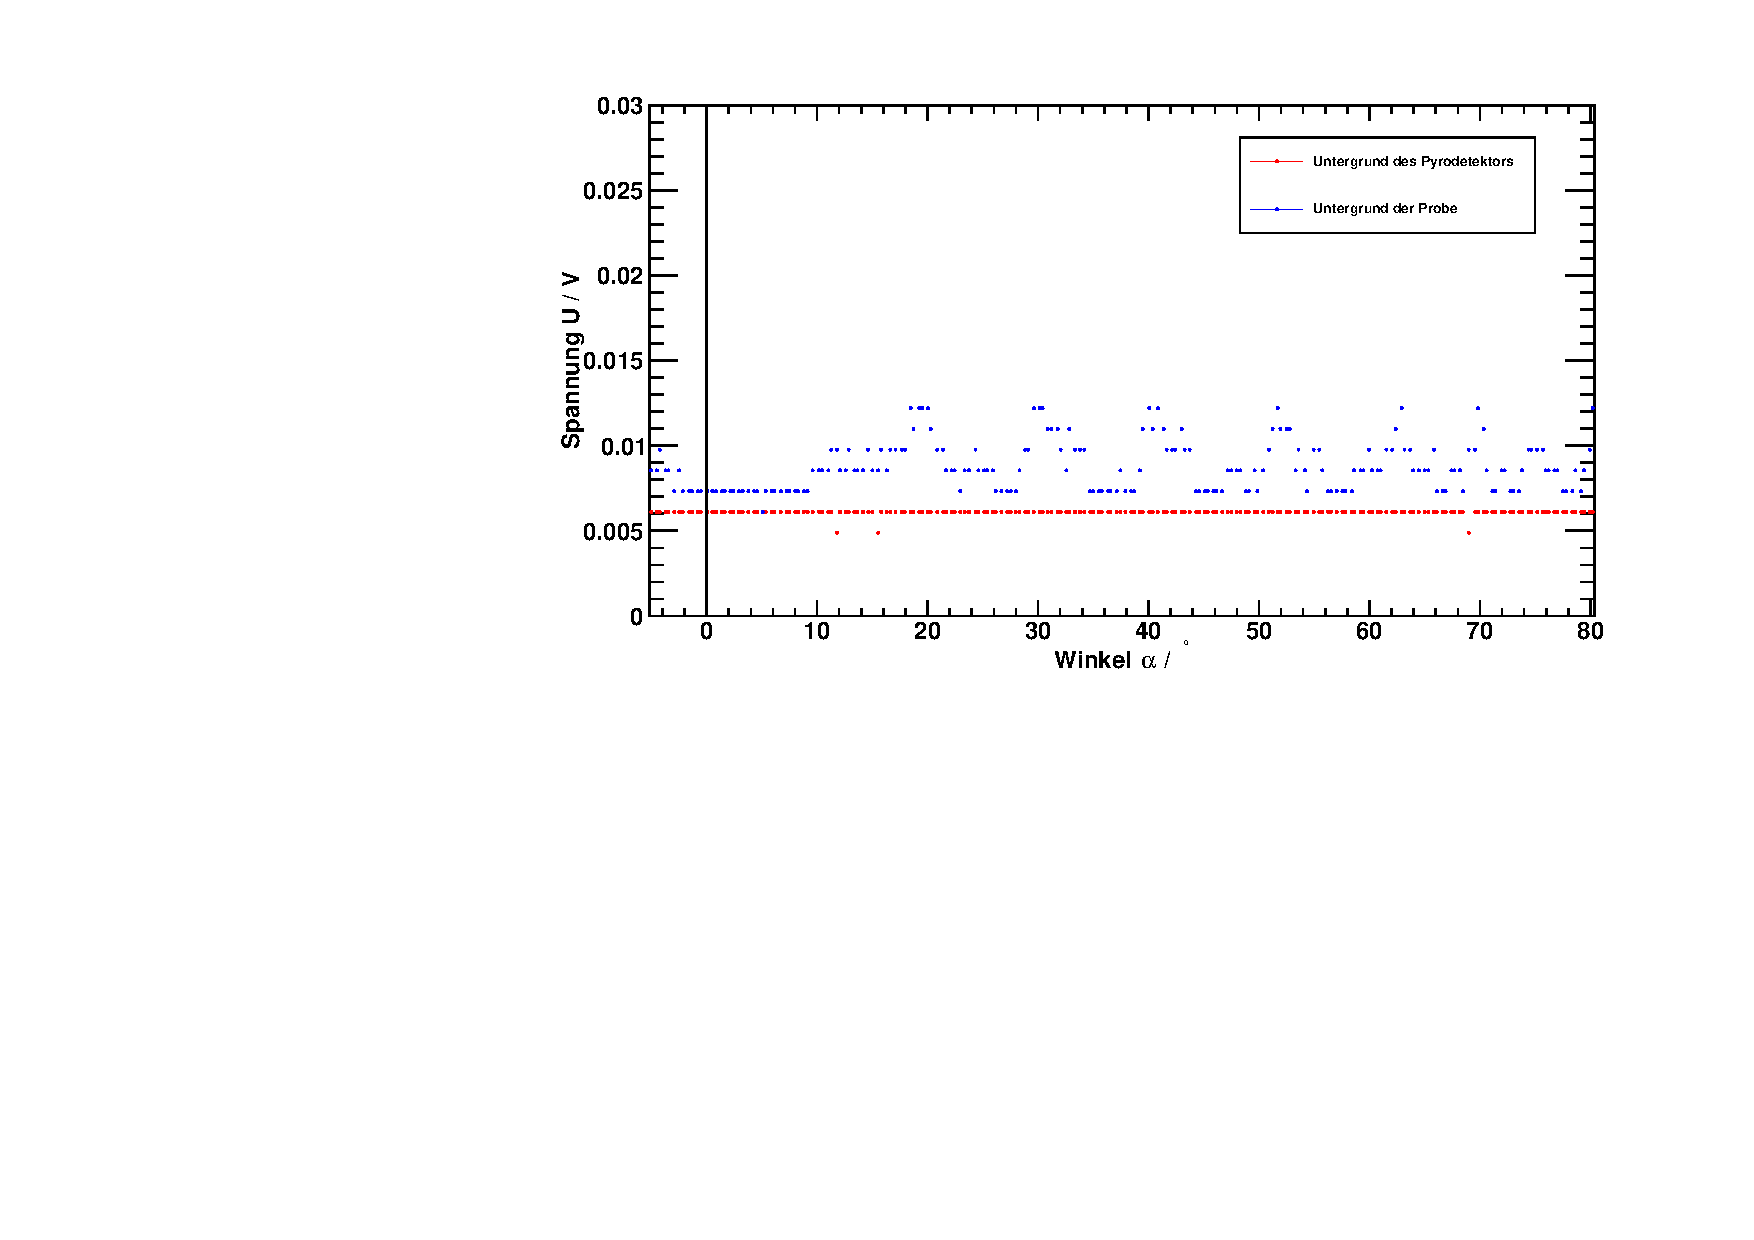
\includegraphics[width=\textwidth]{../img/part1/Si_Untergrund_spectrum.pdf}
  \caption{Untergrund von Pyrodetektor und Siliziumprobe, gemessen mit abgedeckter Lampe.}
  \label{img:si:underground}
\end{center}
\end{figure}

\begin{figure}[H]
\begin{center}
  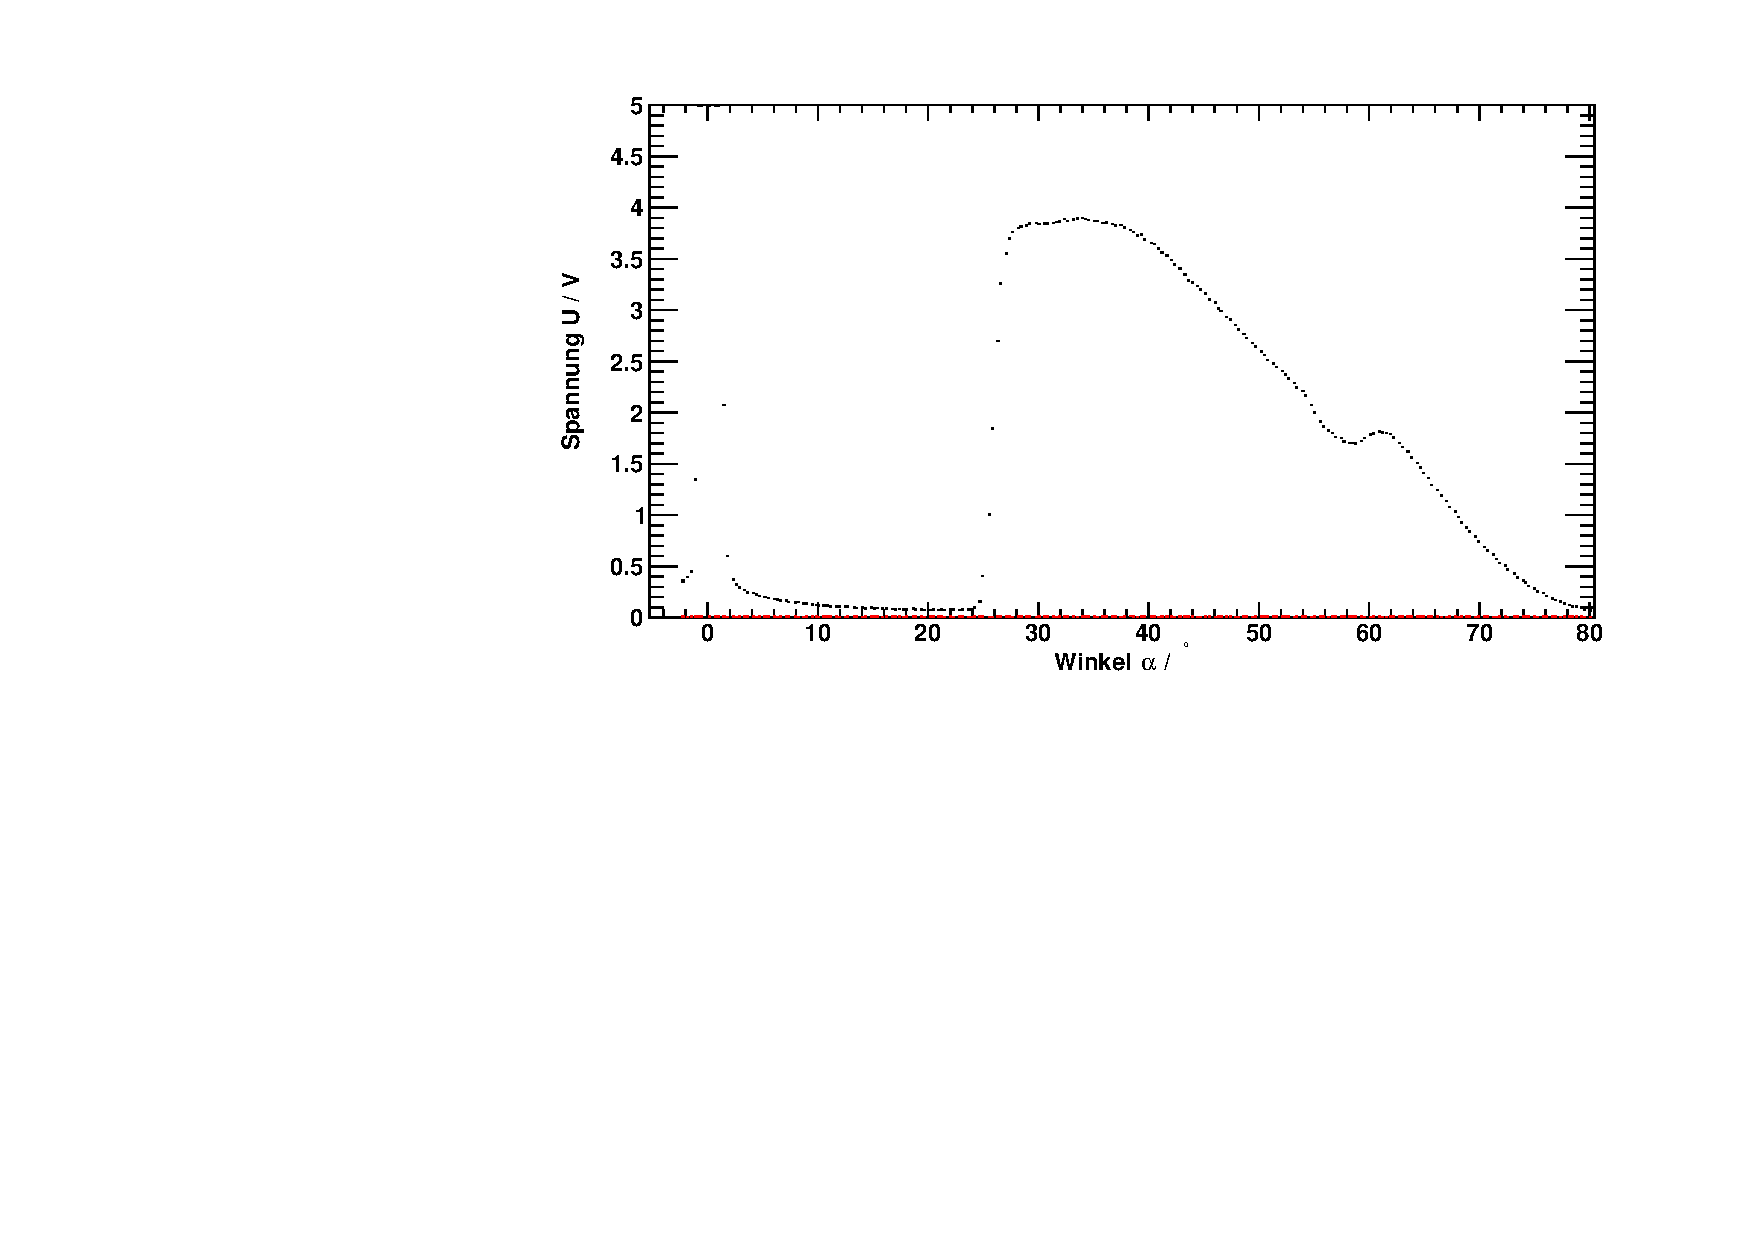
\includegraphics[width=\textwidth]{../img/part1/Si_Lampe_spectrum.pdf}
  \caption{Strahlungsleistung der Lampe in Abhängigkeit des Winkels $alpha$}
  \label{img:si:lampe}
\end{center}
\end{figure}

Die so erhaltenen Intensitäten werden mit den Modellen aus Kapitel \ref{sub:part1:princ:transabs} bei einer Temperatur von $T=300$\,K 
gefittet (\autoref{img:si:transabs}):
\begin{equation}
  \text{Trans}(E) = T_0 \cdot e^{- \alpha(E) \cdot l}, \qquad 
  \text{Abs}(E) = A_0 \cdot e^{- \alpha(E) \cdot d} \left( 1 - e^{- \alpha(E) \cdot (l - d)}  \right) + y_0
\end{equation}

\begin{figure}[H]
\begin{center}
  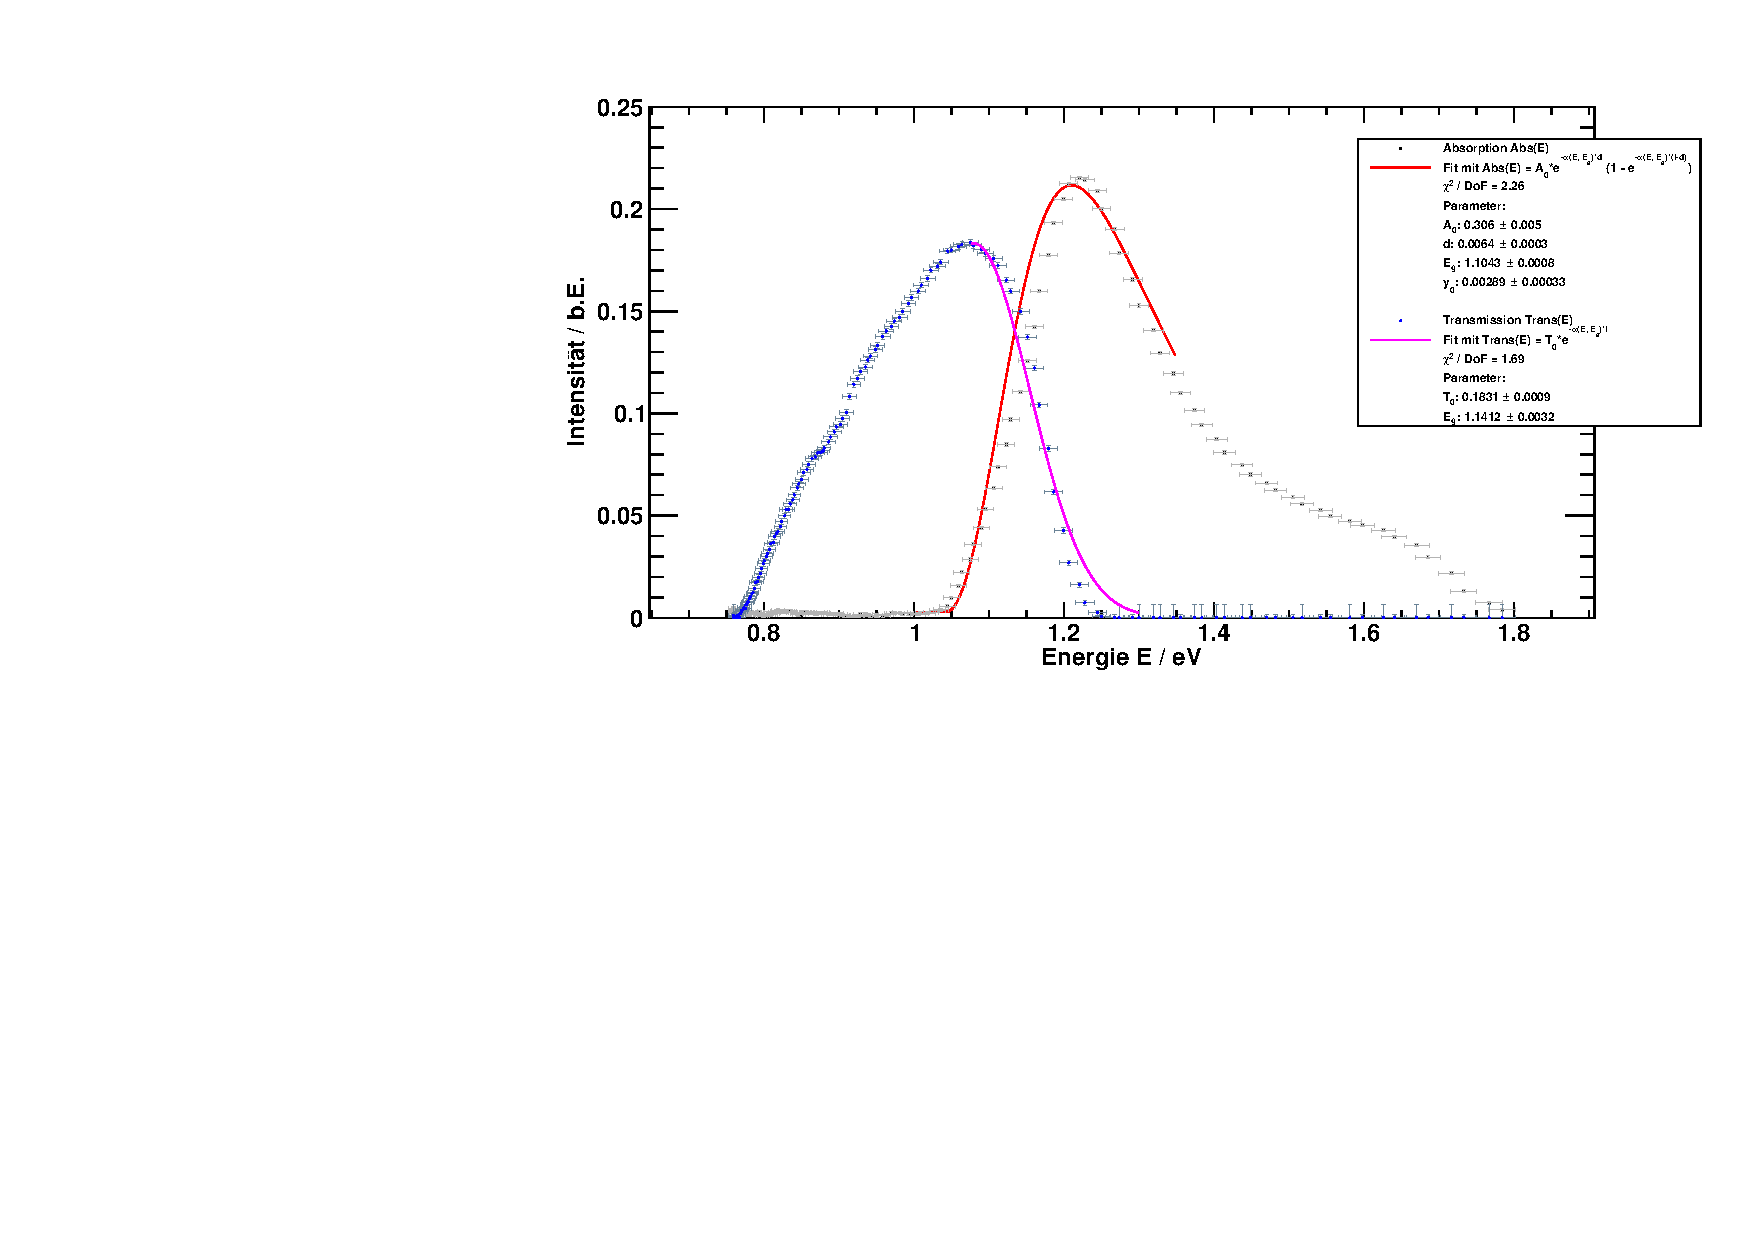
\includegraphics[width=\textwidth]{../img/part1/Si_fit_AbsTrans.pdf}
  \caption{Untergrundbereinigte und normierte Signalintensitäten für die Siliziumprobe.}
  \label{img:si:transabs}
\end{center}
\end{figure}

Man erhält für die Bandlückenenergie von Silizium:
\begin{equation}
\begin{split}
  E_{g, \text{Abs}} &= (1.1043 \pm 0.0008)\,\text{eV} \\
  E_{g, \text{Trans}} &= (1.141 \pm 0.003)\,\text{eV}
\end{split}
\end{equation}
Für den Fehler von $E_g$ muss allerdings noch berücksichtigt werden, dass die endliche Breite der Blende ($d=2$\,cm) und 
des Gitters ($D=2.5$\,cm) nicht eine genaue Energie sondern ein Energieintervall gemessen wird. Nach \cite{staatsex} können 
die Winkel $W_\text{min}$ und $W_\text{max}$ berechnet werden, zwischen denen die Photonen bei einem festen Anstellwinkel $\Phi$ noch 
gemessen werden:
\begin{equation}
\begin{split}
  W_\text{min}(\Phi) &= \Psi + \arcsin \left( \sin(\Psi) - \frac{\frac{D}{2} \cdot \cos(\Phi) + \frac{d}{2} \cdot \cos(\Psi)}{L} \right) \\
  W_\text{max}(\Phi) &= \Psi + \arcsin \left( \sin(\Psi) + \frac{\frac{D}{2} \cdot \cos(\Phi) + \frac{d}{2} \cdot \cos(\Psi)}{L} \right) 
\end{split}
\end{equation}
mit $\Psi=7.5^\circ$ und dem Abstand $L=55$\,cm zwischen Blende und Gitter. \\
Es kann nun der systematische Fehler aus dieser Unschärfe berechnet werden:
\begin{equation}
  s_E = \frac{1}{2} \left( \frac{h \cdot c}{2 \cdot d \cdot \cos(\Psi) \cdot \sin (W_\text{min} / 2)} - \frac{h \cdot c}{2 \cdot d \cdot \cos(\Psi) \cdot \sin (W_\text{max} / 2)} \right) 
\end{equation}
Für den gesamten Fehler auf $E_g$ folgt:
\begin{equation}
  s_{E_g} = \sqrt{s_\text{Fit}^2 + s_E^2}
\end{equation}
Die errechneten Bandlückenenergien können mit \autoref{eq:energy_angle} in den Anstellwinkel $\Phi$ umgerechnet werden. Es folgt für die 
neuen Fehler:
\begin{equation}
\begin{split}
  E_{g, \text{Abs}} &= (1.1043 \pm )\,\text{eV} \\
  E_{g, \text{Trans}} &= (1.141 \pm )\,\text{eV}
\end{split}
\end{equation}
Der gewichtete Mittelwert liefert:
\begin{equation}
  \bar{E}_g = (1.10637 \pm 0.0008)\,\text{eV}
\end{equation}
Die Abweichung vom Literaturwert
\begin{equation}
  E_g^{\text{Lit}} = 1.12\,\text{eV}
\end{equation}
beträgt ca. 1\% des Messwertes. Der Fit liefert nur die statistsichen Fehler 


\subsubsection{Bandlückenenergie von Germanium}
Die Auswertung erfolgt analog zu der Bestimmung der Bandlückenenergie von Silizium. Der Fit (\autoref{img:ge:transabs})
liefert die Bandlückenenergien von Germanium:
\begin{equation}
\begin{split}
  E_{g, \text{Abs}} &= (0.6906 \pm 0.0018)\,\text{eV} \\
  E_{g, \text{Trans}} &= (0.694 \pm 0.002)\,\text{eV}
\end{split}
\end{equation}
%TODO Fehler E_g aus Aufbau
Der gewichtete Mittelwert beträgt
\begin{equation}
  \bar{E}_g = (0.6917 \pm 0.0015)\,\text{eV}
\end{equation}
\begin{equation}
  E_g^{\text{Lit}} = 0.66\,\text{eV}
\end{equation}

\begin{figure}[H]
\begin{center}
  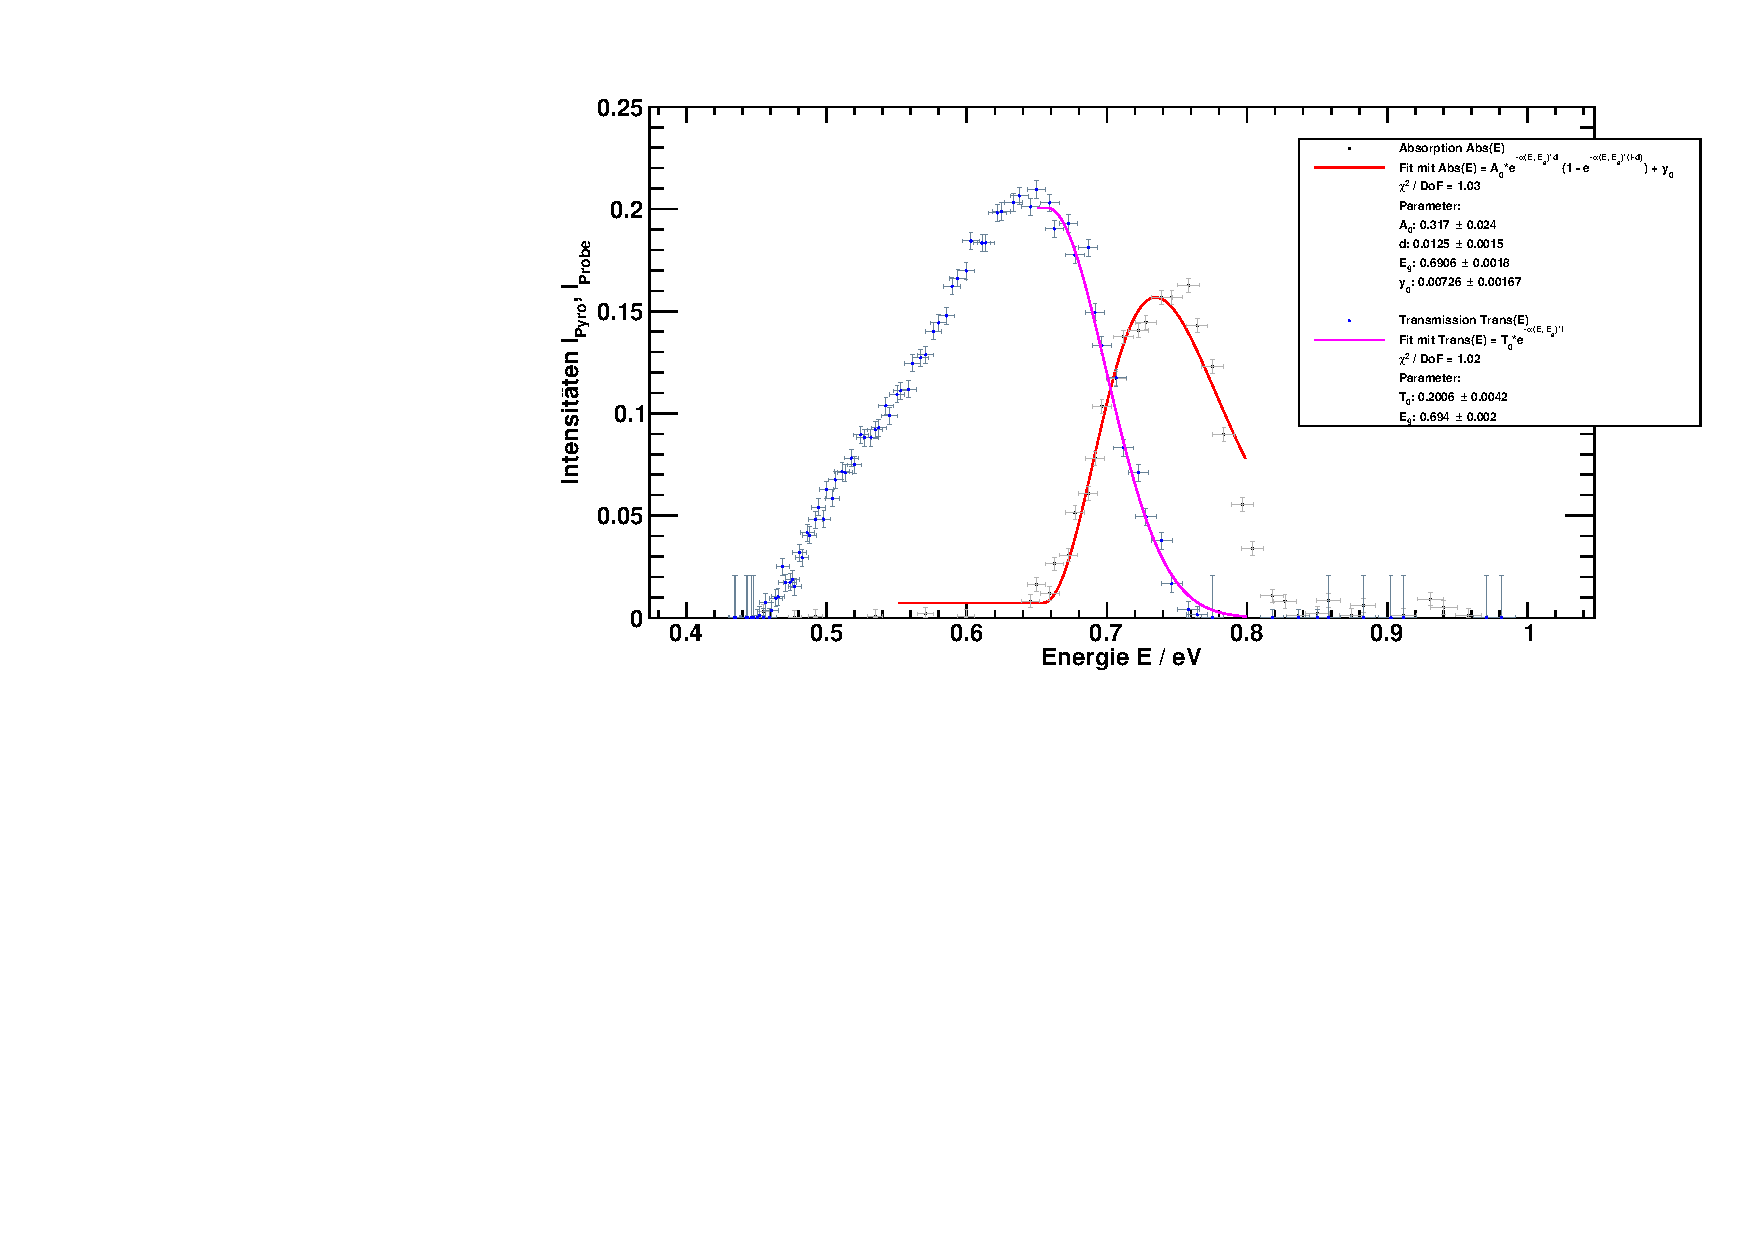
\includegraphics[width=\textwidth]{../img/part1/Ge_fit_AbsTrans.pdf}
  \caption{Untergrundbereinigte und normierte Signalintensitäten für die Germaniumprobe.}
  \label{img:ge:transabs}
\end{center}
\end{figure}


\section{Haynes-Shockley-Experiment}
\subsection{Versuchsaufbau}

\begin{figure}[H]
\begin{center}
  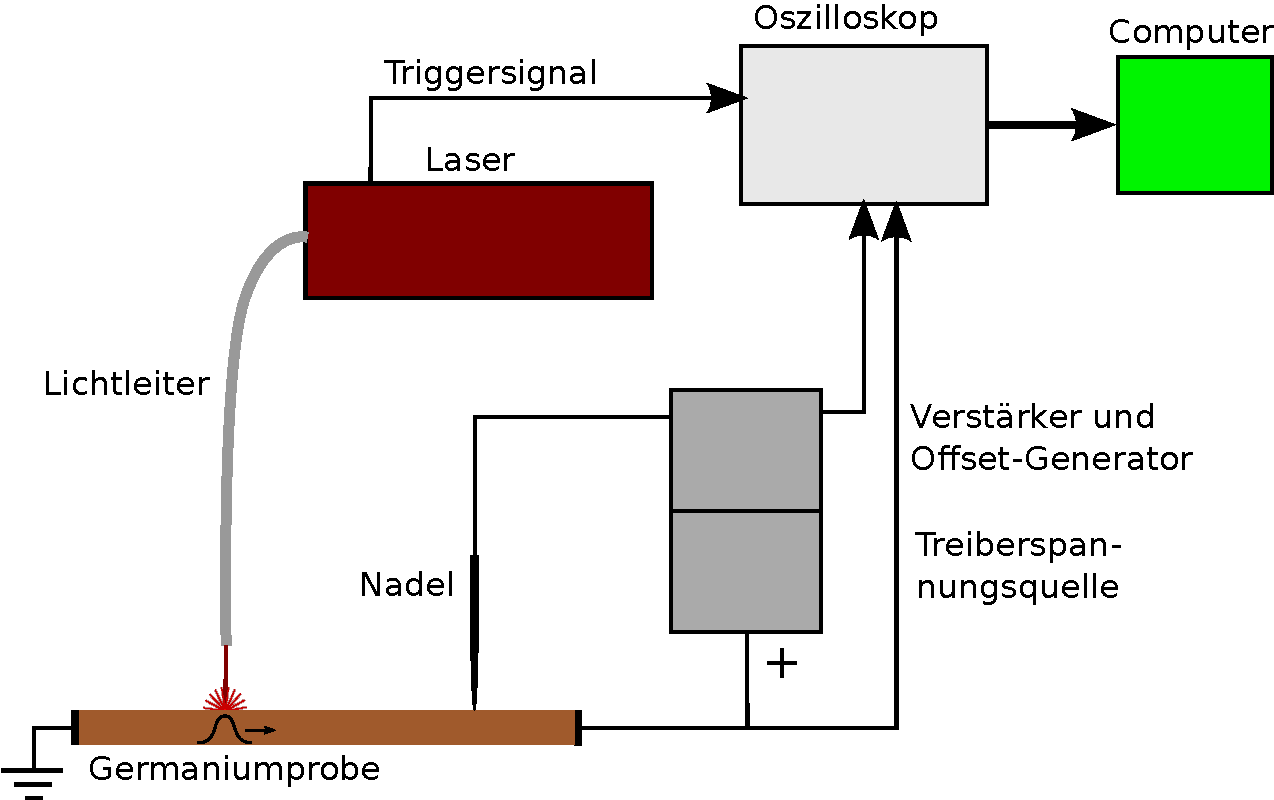
\includegraphics[width=0.75\textwidth]{../img/aufbau1.pdf}
  \caption{Aufbau für das Haynes-Shockley-Experiment zur Messung der Drift, Diffusion und Rekombination einer
  Elektronenwolke, die von einem Laserpuls erzeugt wird.}
  \label{img:lab}
\end{center}
\end{figure}
\subsection{Versuchsdurchführung}

Am Aufbau werden zwei Messreihen durchgeführt:\\
Zuerst wird das Signal am Oszilloskop in Abhängigkeit der Entfernung Lichtleiter-Nadel untersucht.
Die Entfernung (Anzeige auf der Skala) wird zwischen 0\,mm und 10\,mm in 1\,mm-Schritten variiert.
Es liegt immer die maximal mögliche Treibspannung (50\,V) an.
Bei jeder Messung wird der Offset des Signals so eingestellt,
dass es gut am Oszilloskop ablesbar ist und die Daten vom Oszilloskop gespeichert.
Zusätzlich wird mit einer Schiebelehre der Offset zwischen der Mitte des Lichtleiters und der Nadel bestimmt,
wenn die Entfernungsskala auf 0\,mm eingestellt ist.\\
Bei der zweiten Messreihe wird der Abstand der Nadel konstant auf XXX
%TODO Abstand
gehalten und der Wert der Treibspannung in 3\,V-Schritten zwischen 20\,V und 50\,V variiert.
Auch hier wird für jede Messung am Oszilloskop eine geeignete Einstellung gesucht und die Daten gespeichert.
\subsection{Messergebnisse und Auswertung}
\subsubsection{Bestimmung des Offsets \texorpdfstring{$x_0$}{x0}}
Der Abstand zwischen Messspitze und Lichtleiter wurde aufgrund des Versuchsaufbaus mit einem Offset $x_0$ gemessen. Der Offset wurde separat 
von jedem Versuchspartner einmal bestimmt. Aus den Messwerten wurde der Mittelwert bestimmt (Fehler der Einzelmessung $s_{x_i} = 0.2$\,mm):
\begin{equation}
  x_0 = (1.25 \pm 0.14)\,\text{mm}
\end{equation}
\subsubsection{Variation der Nadelposition \texorpdfstring{$d$}{d}}

\begin{figure}[H]
\begin{center}
  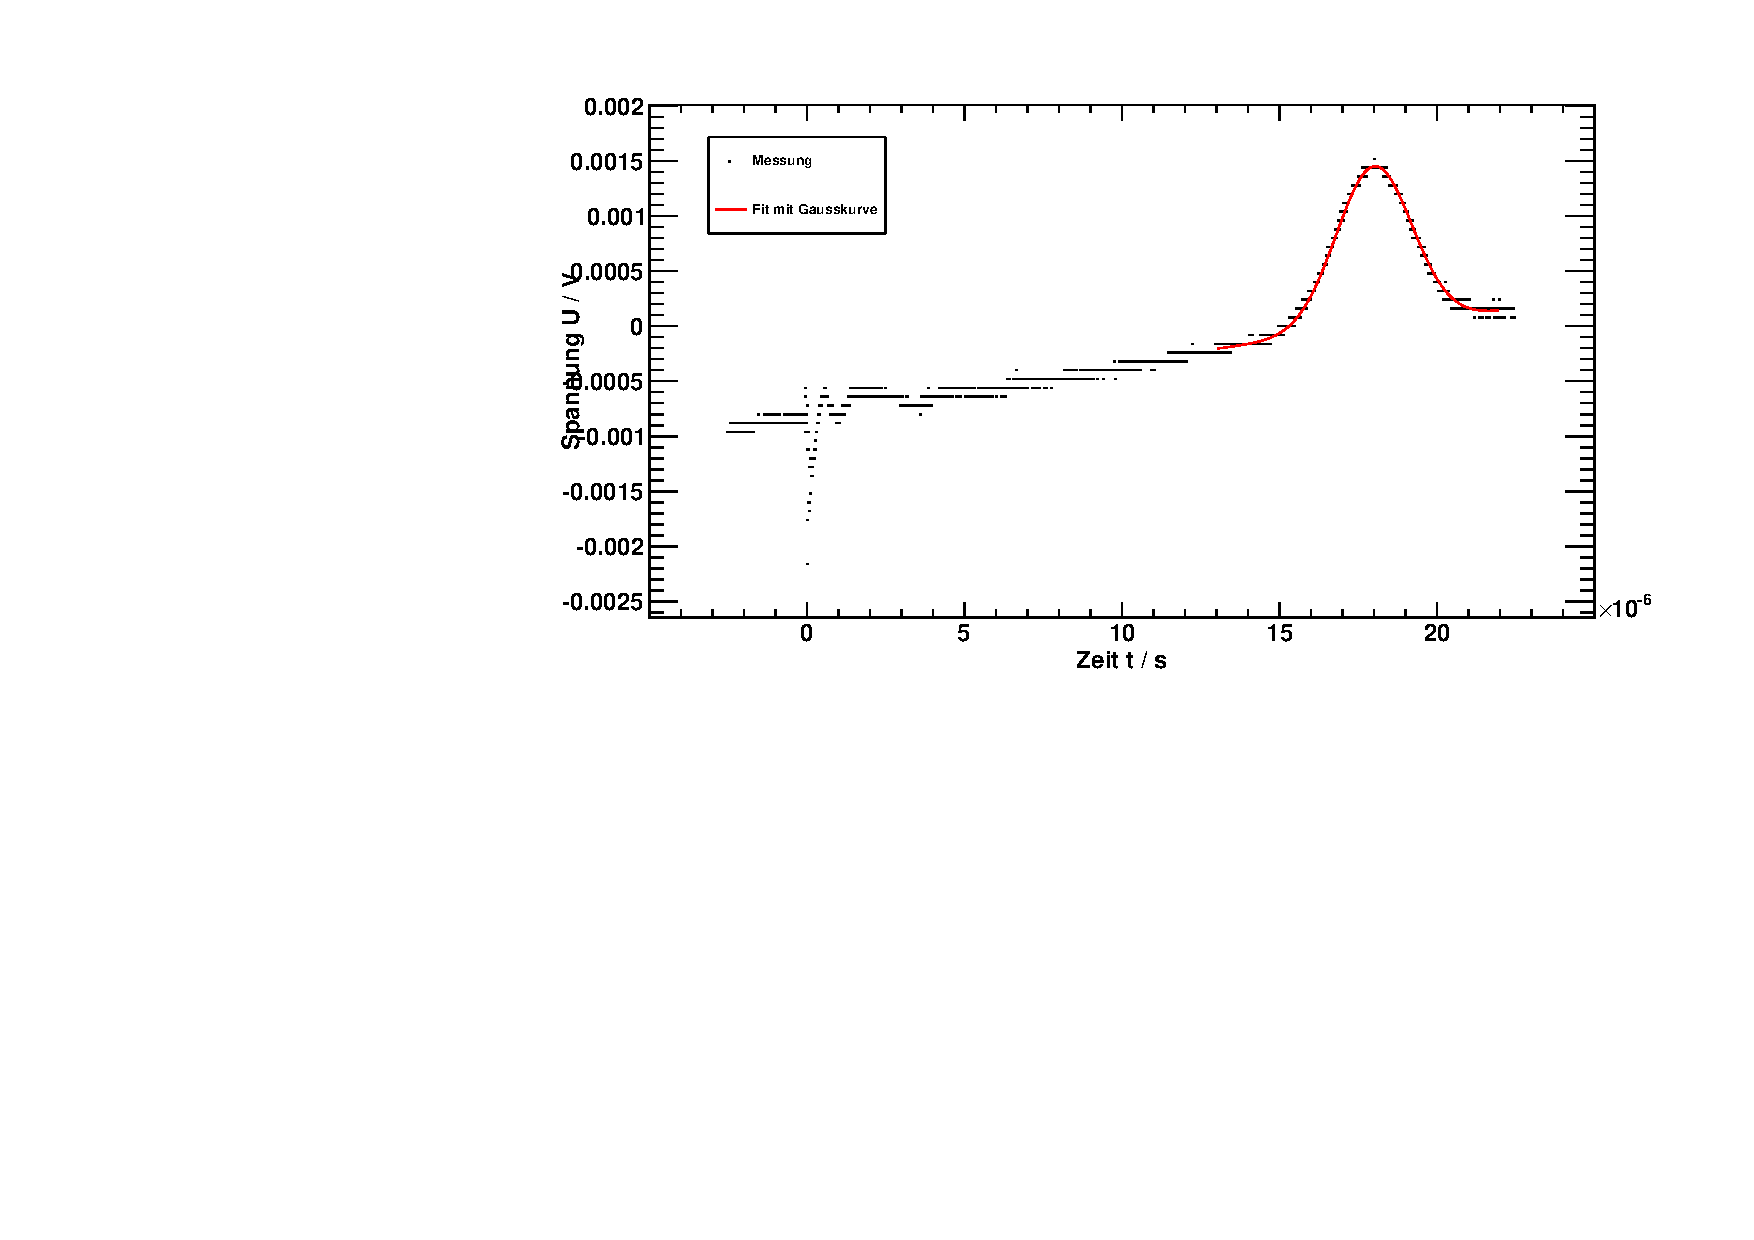
\includegraphics[width=\textwidth]{../img/part2/dist02.pdf}
  \caption{Gaußfit mit linearem Untergrund des Peaks bei $d=8.03$\,mm.}
  \label{img:d:exfit}
\end{center}
\end{figure}
\autoref{img:d:exfit} zeigt einen beispielhaften Fit in dieser Messreihe. Insgesamt wurden so 11 Messungen gefittet. Die Gleichung ergibt sich 
aus \autoref{eq:gauss} und einem linearen Untergrund:
\begin{equation}
  U(t) = a + b \cdot t + A \cdot \frac{1}{\sqrt{2  \pi  \cdot \sigma^2}} \cdot
  e^{-\frac{1}{2} \left( \frac{t - t_{\text{c}}}{\sigma^2} \right)^2}
\end{equation}
Die untergrundbereinigten Messungen (ohne Fits) sind in \autoref{img:distances} dargestellt.
\begin{figure}[H]
\begin{center}
  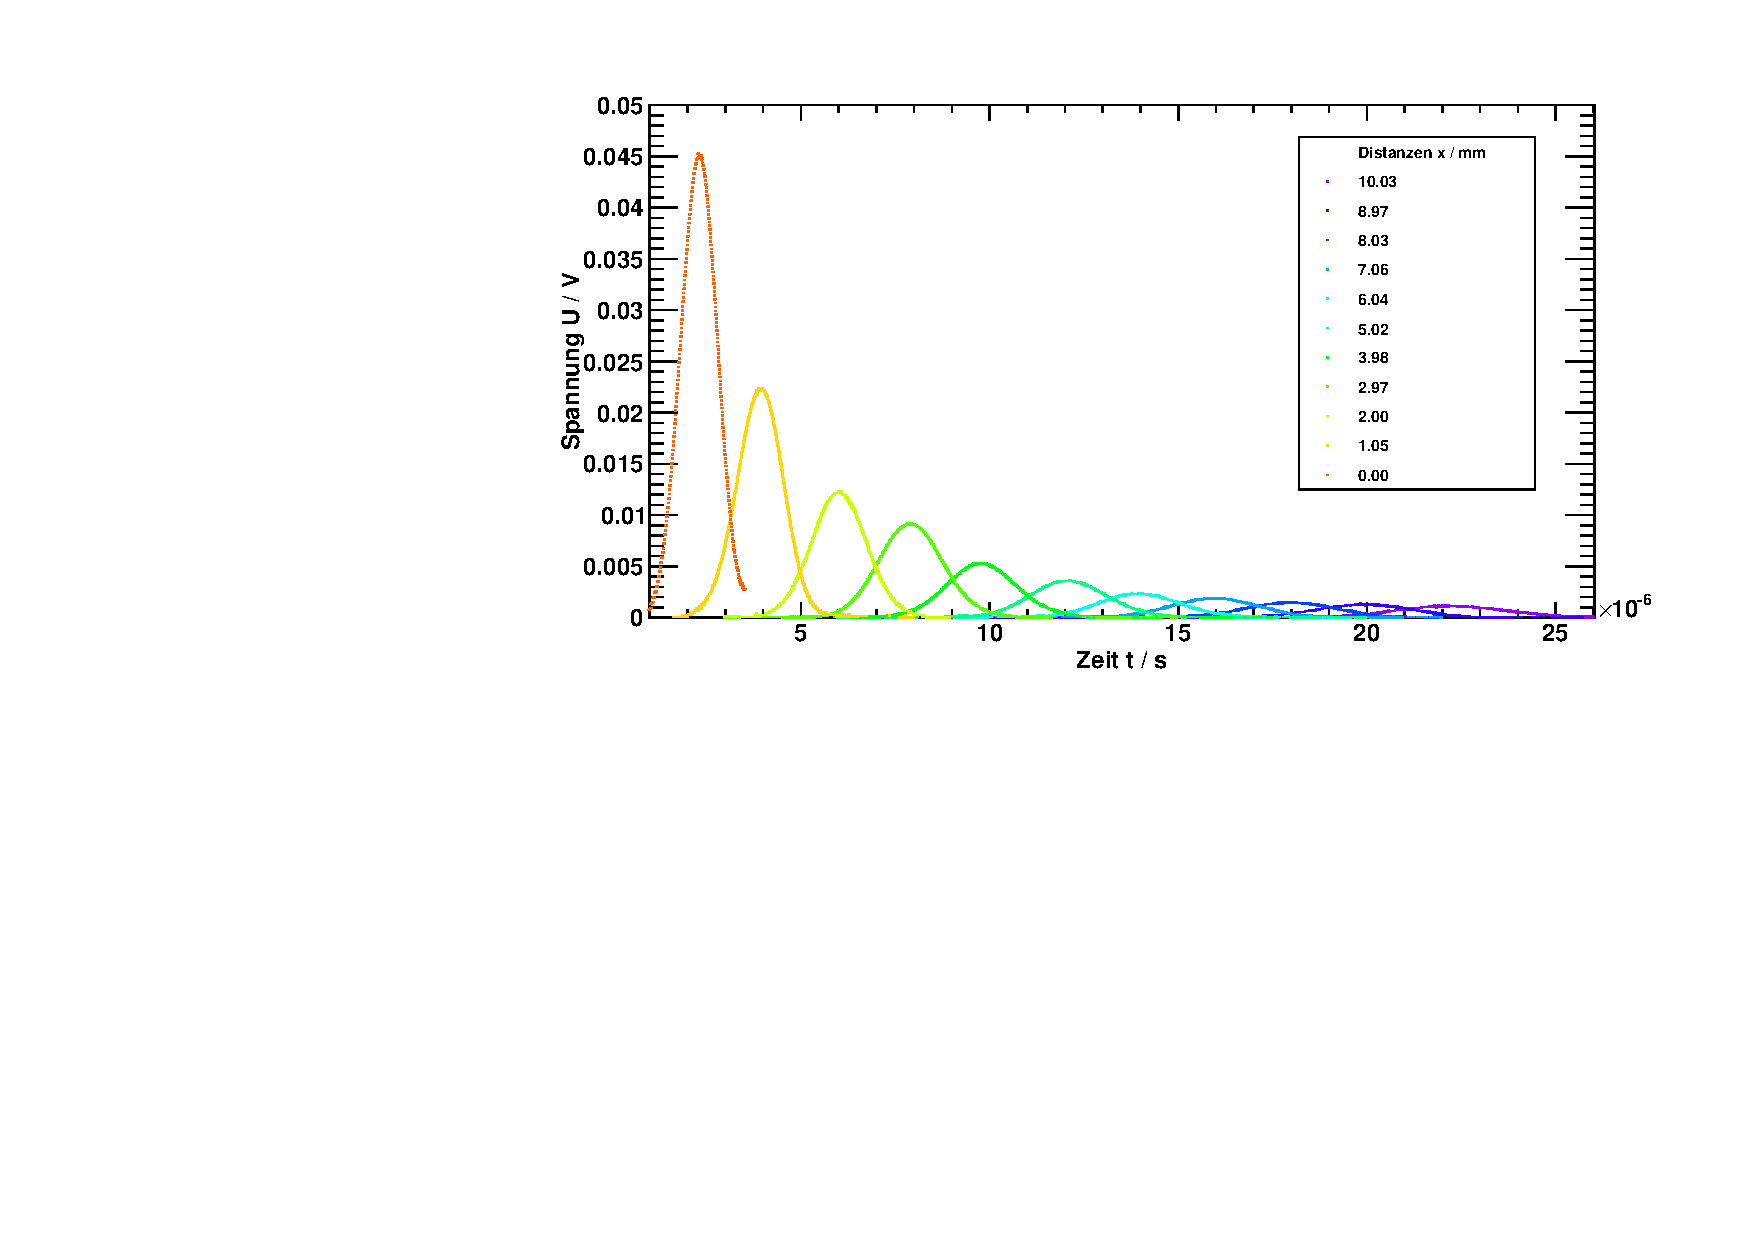
\includegraphics[width=\textwidth]{../img/part2/distances.pdf}
  \caption{Zeitlicher Verlauf der Spannungen für verschiedene Abstände $d$ zwischen Messspitze und Lichtleiter.}
  \label{img:distances}
\end{center}
\end{figure}

\paragraph{Bestimmung der Ladungsträgermobilität $\mu$}
Für jeden Gaußfit wird die Entfernung $d$ zwischen Lichtleiter und Nadelspitze über dem Zeitpunkt des Maximumdurchlaufs $t_{\text{c}}$ 
aufgetragen (\autoref{img:dist:fitxc}). Der so erhaltene Graph wird mit einer Geraden gefittet.

\begin{figure}[H]
\begin{center}
  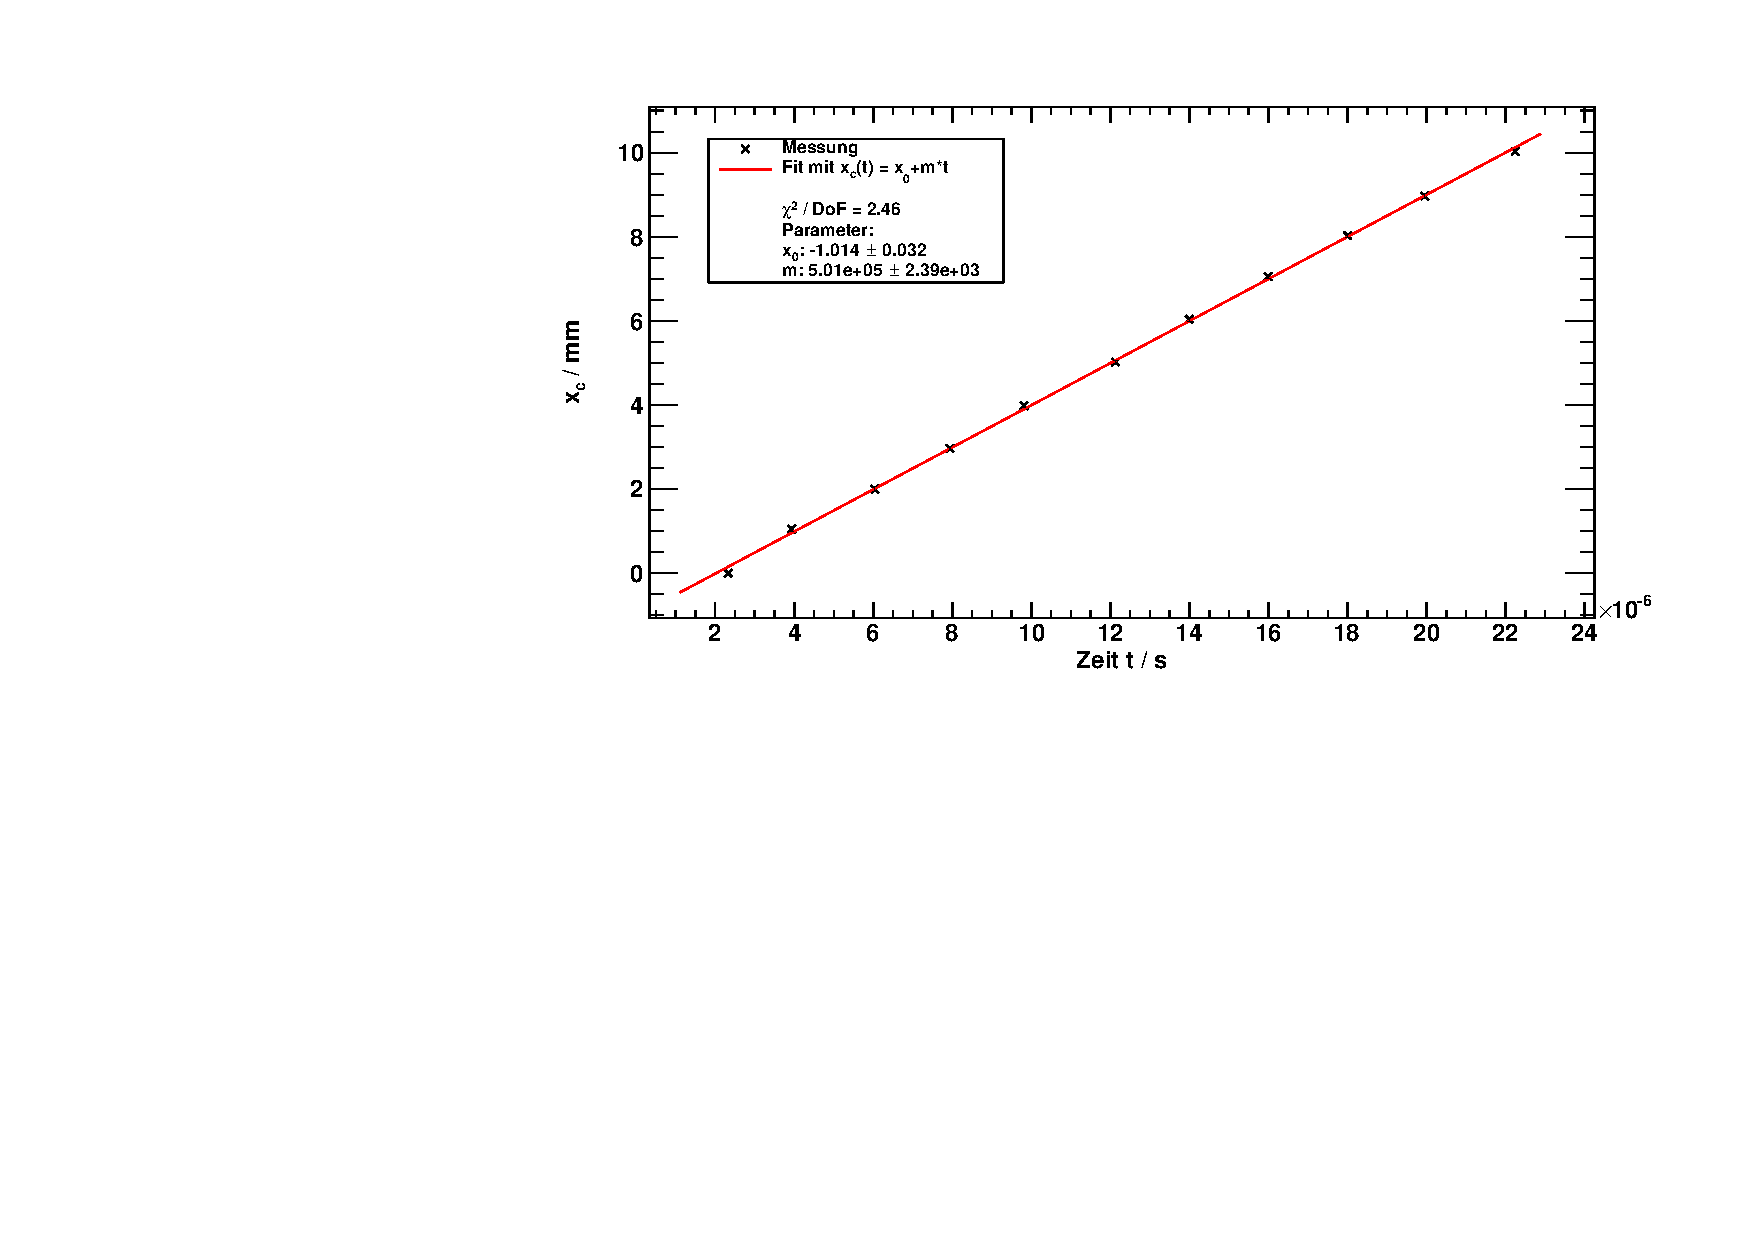
\includegraphics[width=\textwidth]{../img/part2/dist_fitXc.pdf}
  \caption{Ausgleichsgerade} %TODO caption
  \label{img:dist:fitxc}
\end{center}
\end{figure}

Der Betrag des Achsenabschnitts $|x_0| = (1.01 \pm 0.03)$\,mm stimmt innerhalb von zwei Standardabweichungen mit dem oben bestimmten Wert des 
Offsets überein.\\
Die Steigung $m$ ist das Produkt aus Ladungsträgermobilität und angelegtem E-Feld 
(nach \autoref{eq:gaus:params}):
\begin{equation}
  \label{eq:efield}
  m = \mu \cdot E = \mu \cdot \frac{U}{d}
\end{equation}
mit $U = (48.8 \pm 0.4)$\,V und $d=30$\,mm. Man erhält mit Gauß'scher Fehlerfortpflanzung für $\mu$
\begin{equation}
  \mu = (3079 \pm 29)\,\frac{\text{cm}^2}{\text{V} \cdot \text{s}}
\end{equation}
Dieser Wert ist gegenüber dem Literaturwert
\begin{equation}
  \mu^{\text{Lit}} = 3900\,\frac{\text{cm}^2}{\text{V} \cdot \text{s}}
\end{equation}
stark erniedrigt. Dies kann mit Gitterfehlern an der Probenoberfläche erklärt werden, da diese die Ladungsträgermobilität verringern.

\paragraph{Bestimmung der Diffusionskonstanten $D_\text{n}$}
Die aus den Fits erhaltenen Standardabweichungen $\tilde{\sigma}$ werden gemäß \autoref{eq:gauss} mit $\mu \cdot E$ multipliziert und 
in \autoref{img:dist:fitsigma} über $t_c$ aufgetragen. Die Beweglichkeit $\mu$ erhält man von oben und das E-Feld wird analog zu \autoref{eq:efield} berechnet.
Der Fit erfolgt mit \autoref{eq:gaus:params} und einem Zeitoffset $t_0$.
\begin{equation}
  \sigma(t) = \sqrt{2 \cdot D_\text{n} \cdot (t-t_0)}
\end{equation}
Der Offset könnte von einer ungenauen Triggerung auf den Laserpuls oder seine Ausdehnung verursacht werden. \\
Bei dem Fit wurde der letzte Messwert ($t=22$\,\textmu s) nicht berücksichtigt, da er offensichtlich weit neben dem Modell liegt.

\begin{figure}[H]
\begin{center}
  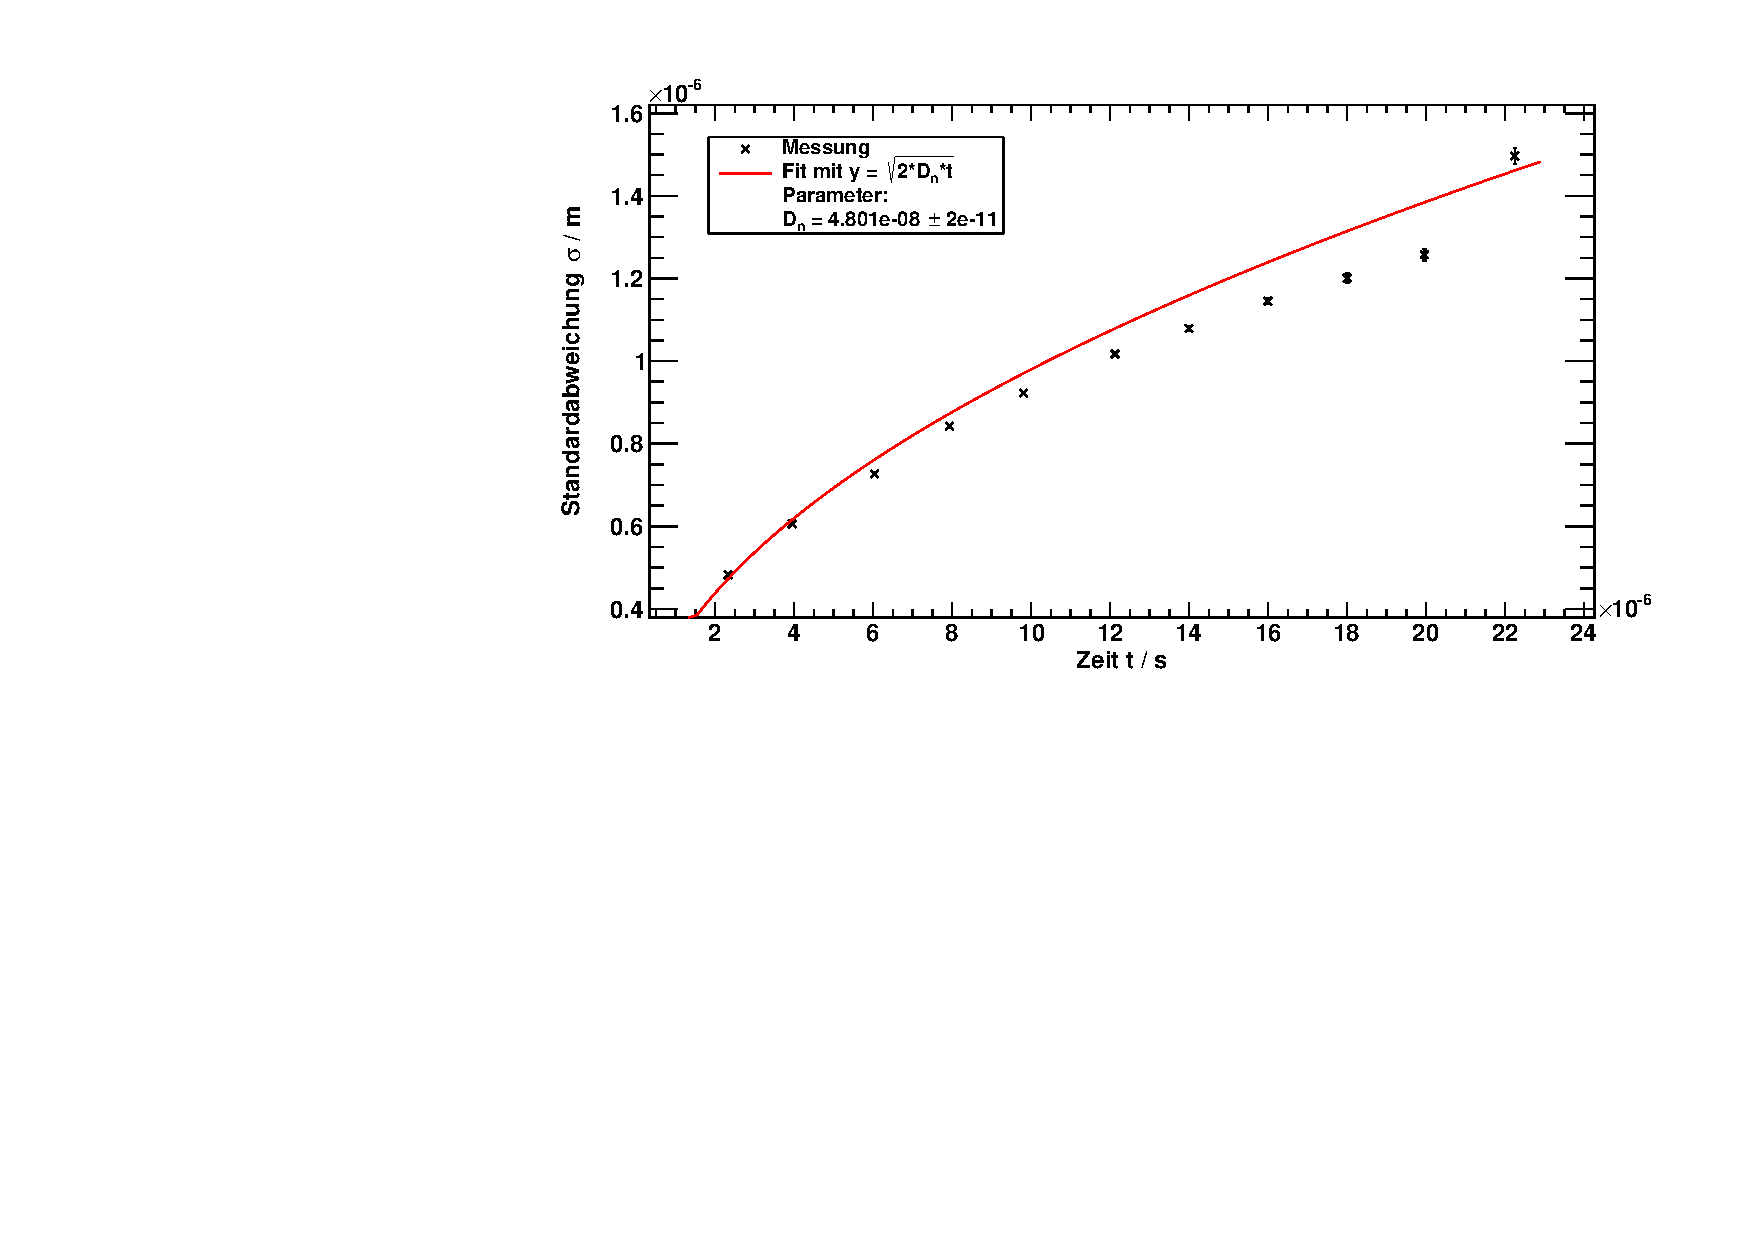
\includegraphics[width=\textwidth]{../img/part2/dist_fitSigma.pdf}
  \caption{caption}
  \label{img:dist:fitsigma}
\end{center}
\end{figure}
Man erhält für die Diffusionskonstante:
\begin{equation}
  D_\text{n} = (99.6 \pm 1.1)\,\frac{\text{cm}^2}{\text{s}}
\end{equation}
Sie stimmt innerhalb von zwei Standardabweichungen mit dem Literaturwert überein. 
\begin{equation}
  D_\text{n}^{\text{Lit}} = 101\,\frac{\text{cm}^2}{\text{s}} 
\end{equation}

\paragraph{Bestimmung der mittleren Lebensdauer $\tau_\text{n}$}
Für die Bestimmung der mittleren Lebensdauer wird der Zusammenhang aus \autoref{eq:gaus:params} mit einen konstanten Offset verwendet:
\begin{equation}
  A(t) = C \cdot e^{- \frac{t}{\tau_\text{n}}} + a
\end{equation}
Der Offset gibt einen systematischen Fehler an, der durch einen Teil des Untergrundes, welcher nicht mit der linearen Funktion oben 
berücksichtigt wurde, verursacht werden könnte.

\begin{figure}[H]
\begin{center}
  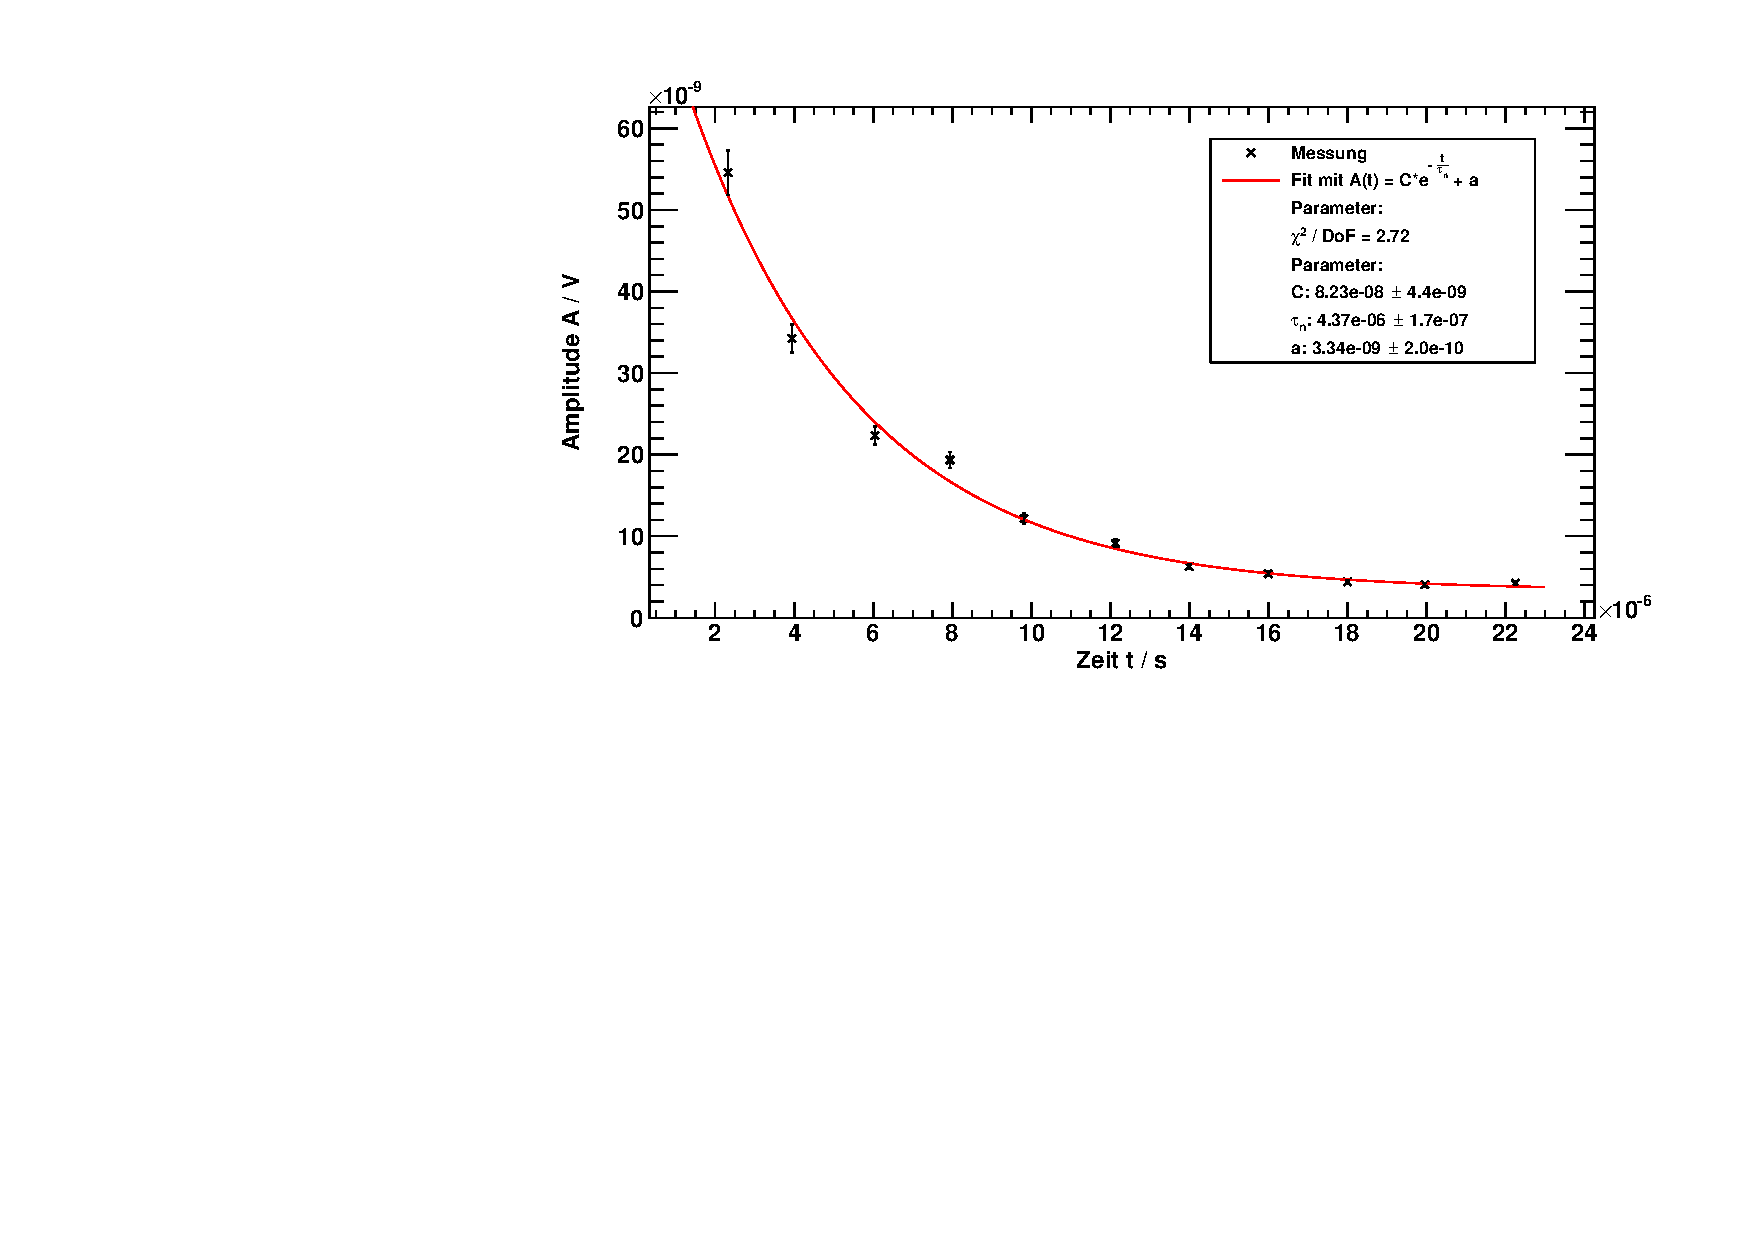
\includegraphics[width=\textwidth]{../img/part2/dist_fitA.pdf}
  \caption{caption}
  \label{img:dist:fita}
\end{center}
\end{figure}
Der Fit liefert für die mittlere Lebensdauer:
\begin{equation}
  \tau_\text{n} = (4.37 \pm 0.17)\,\text{\textmu s}
\end{equation}
Dieser Wert liegt weit unter dem Literaturwert. Die Ursache dafür ist Rekombination der Ladungsträger an oberflächlichen Gitterfehlern.
\begin{equation}
  \tau_\text{n}^\text{Lit} = (45 \pm 2)\,\text{\textmu s}
\end{equation}


\subsubsection{Variation der Treibspannung \texorpdfstring{$U_T$}{U\_T}}

\begin{figure}[H]
\begin{center}
  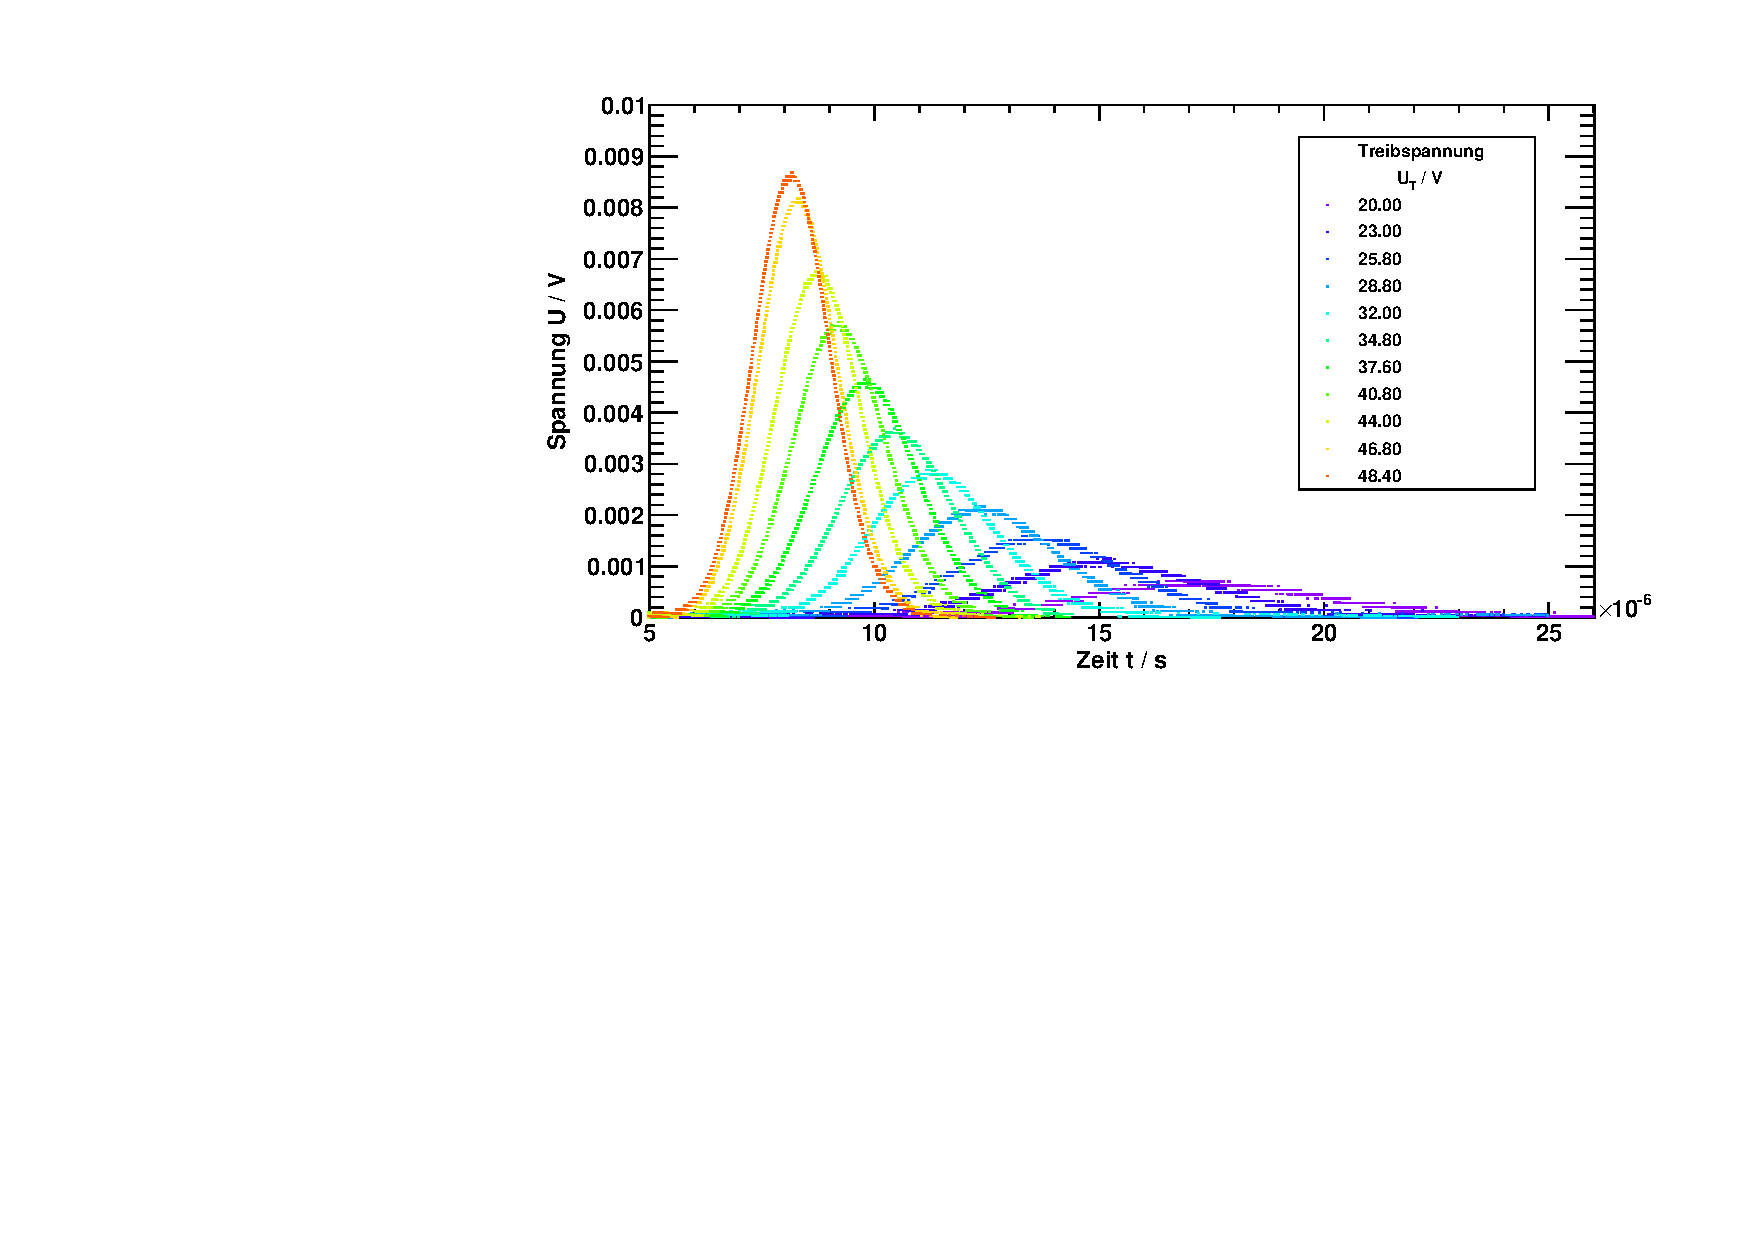
\includegraphics[width=\textwidth]{../img/part2/voltages.pdf}
  \caption{Zeitlicher Verlauf der Spannungen für verschiedene Treibspannungen $U_T$.}
  \label{img:volts}
\end{center}
\end{figure}

\paragraph{Bestimmung der Ladungsträgermobilität $\mu$} 
Platzhalter

\begin{figure}[H]
\begin{center}
  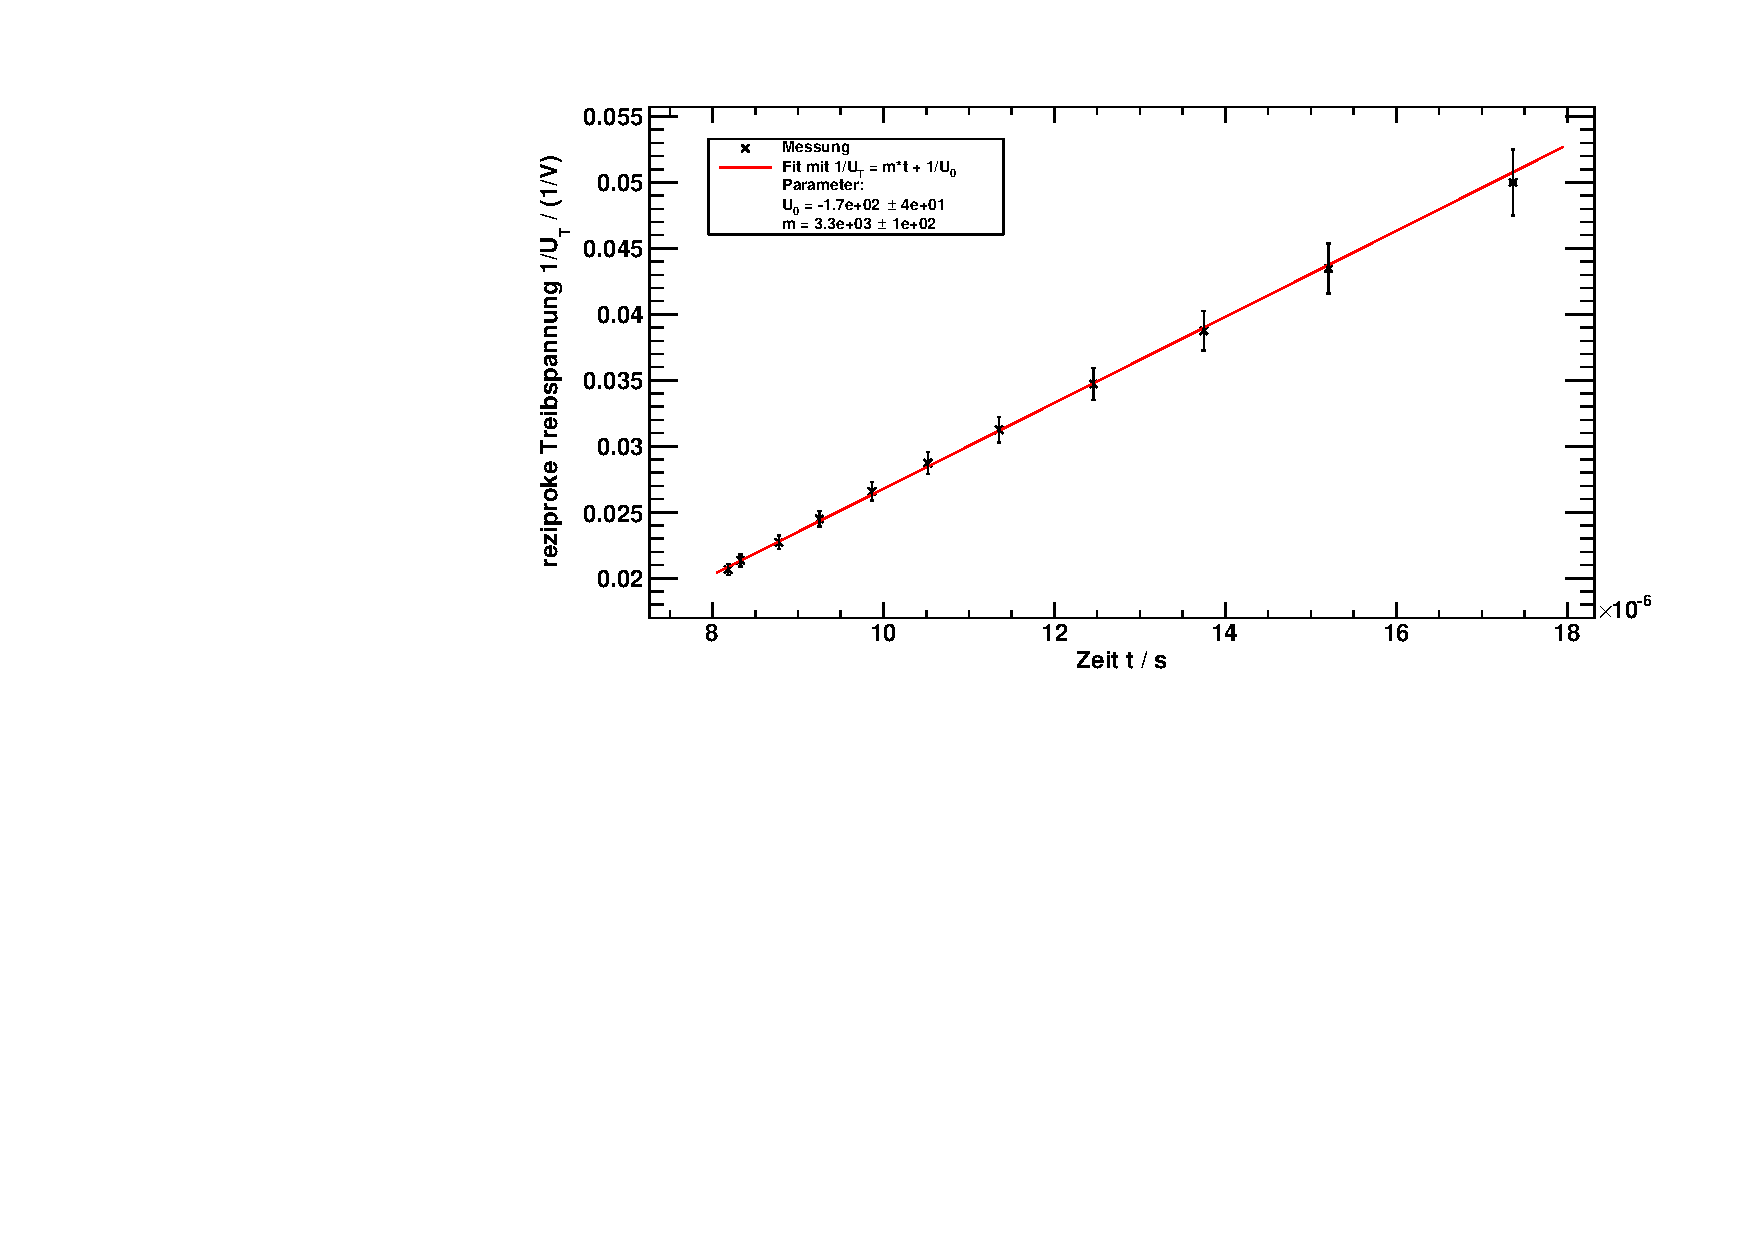
\includegraphics[width=\textwidth]{../img/part2/volt_fitXc.pdf}
  \caption{caption}
  \label{img:volt:fitxc}
\end{center}
\end{figure}

\paragraph{Bestimmung der Diffusionskonstanten $D_\text{n}$}
Platzhalter

\begin{figure}[H]
\begin{center}
  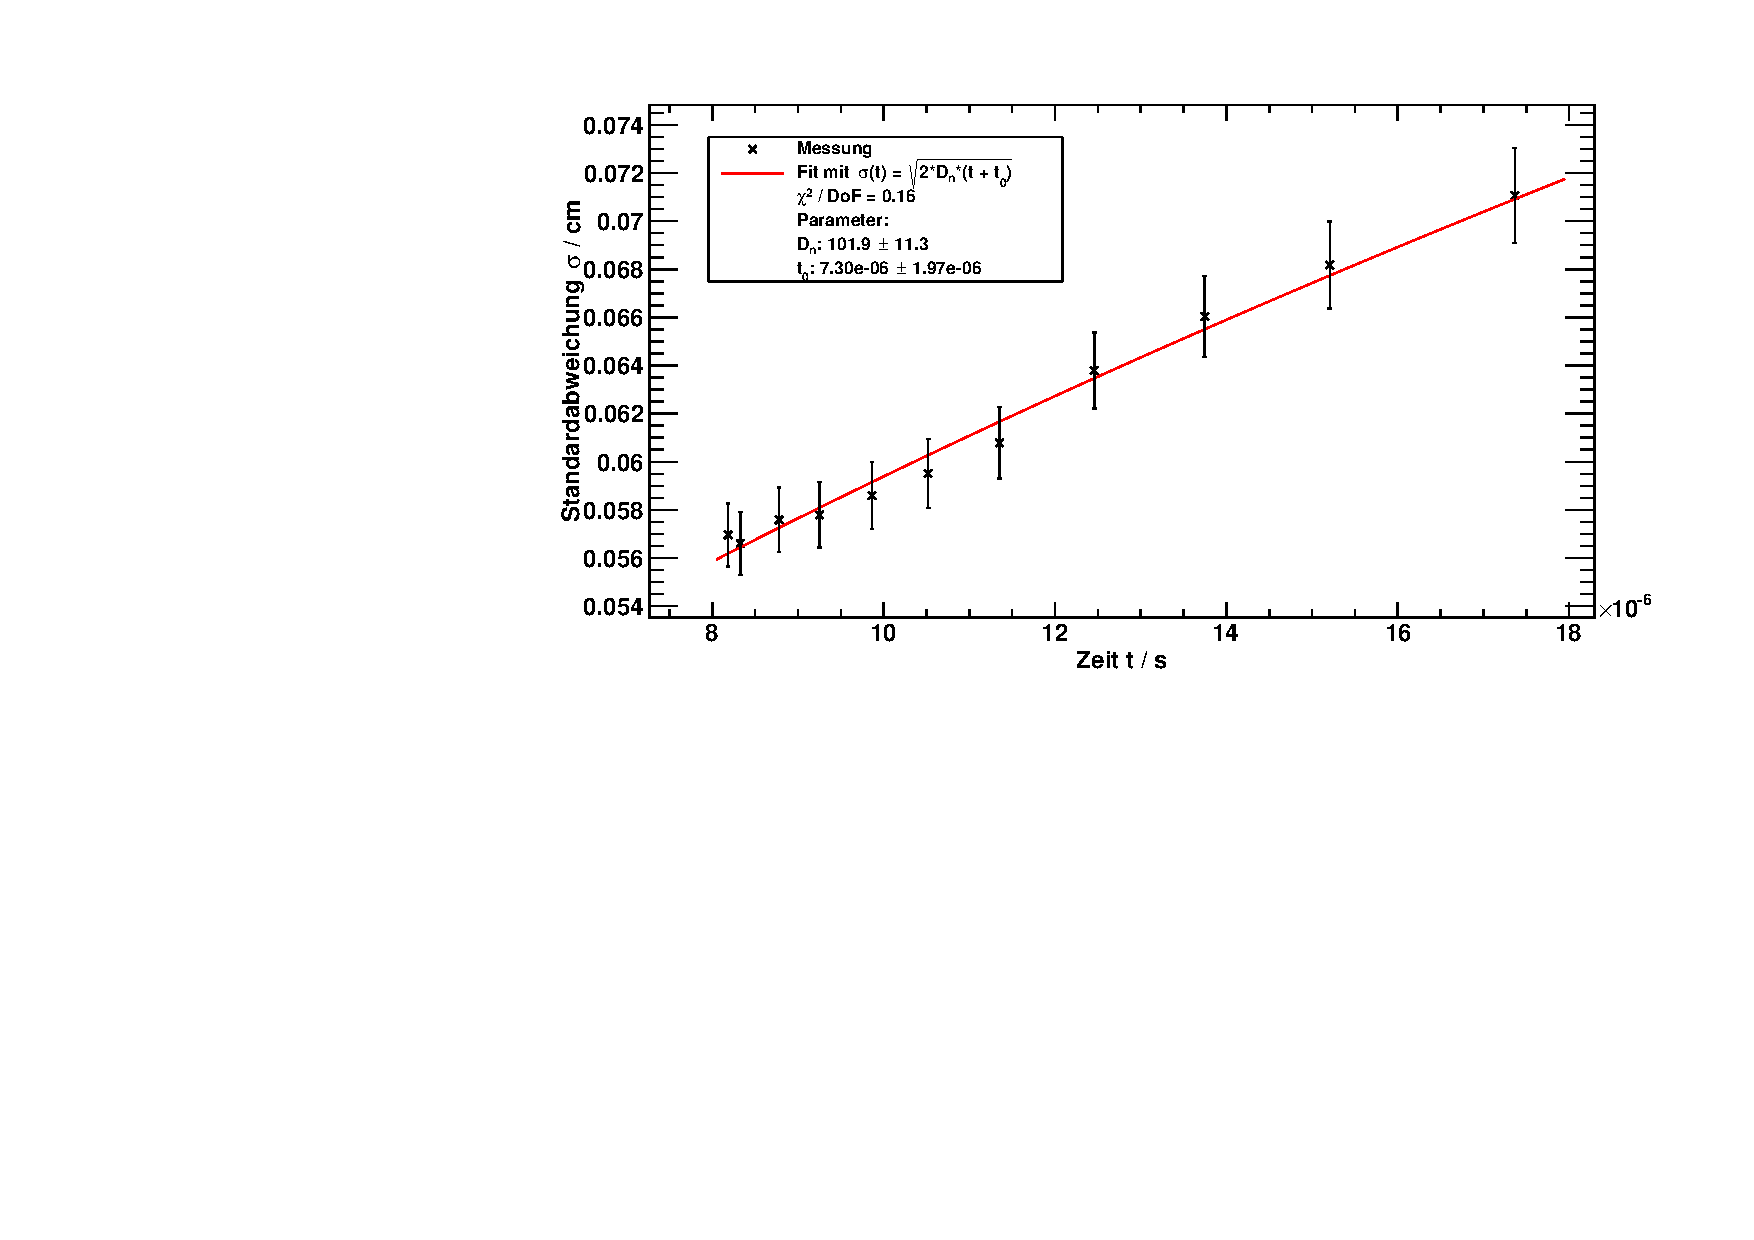
\includegraphics[width=\textwidth]{../img/part2/volt_fitSigma.pdf}
  \caption{caption}
  \label{img:volt:fitsigma}
\end{center}
\end{figure}

\paragraph{Bestimmung der mittleren Lebensdauer $\tau_\text{n}$}
Platzhalter

\begin{figure}[H]
\begin{center}
  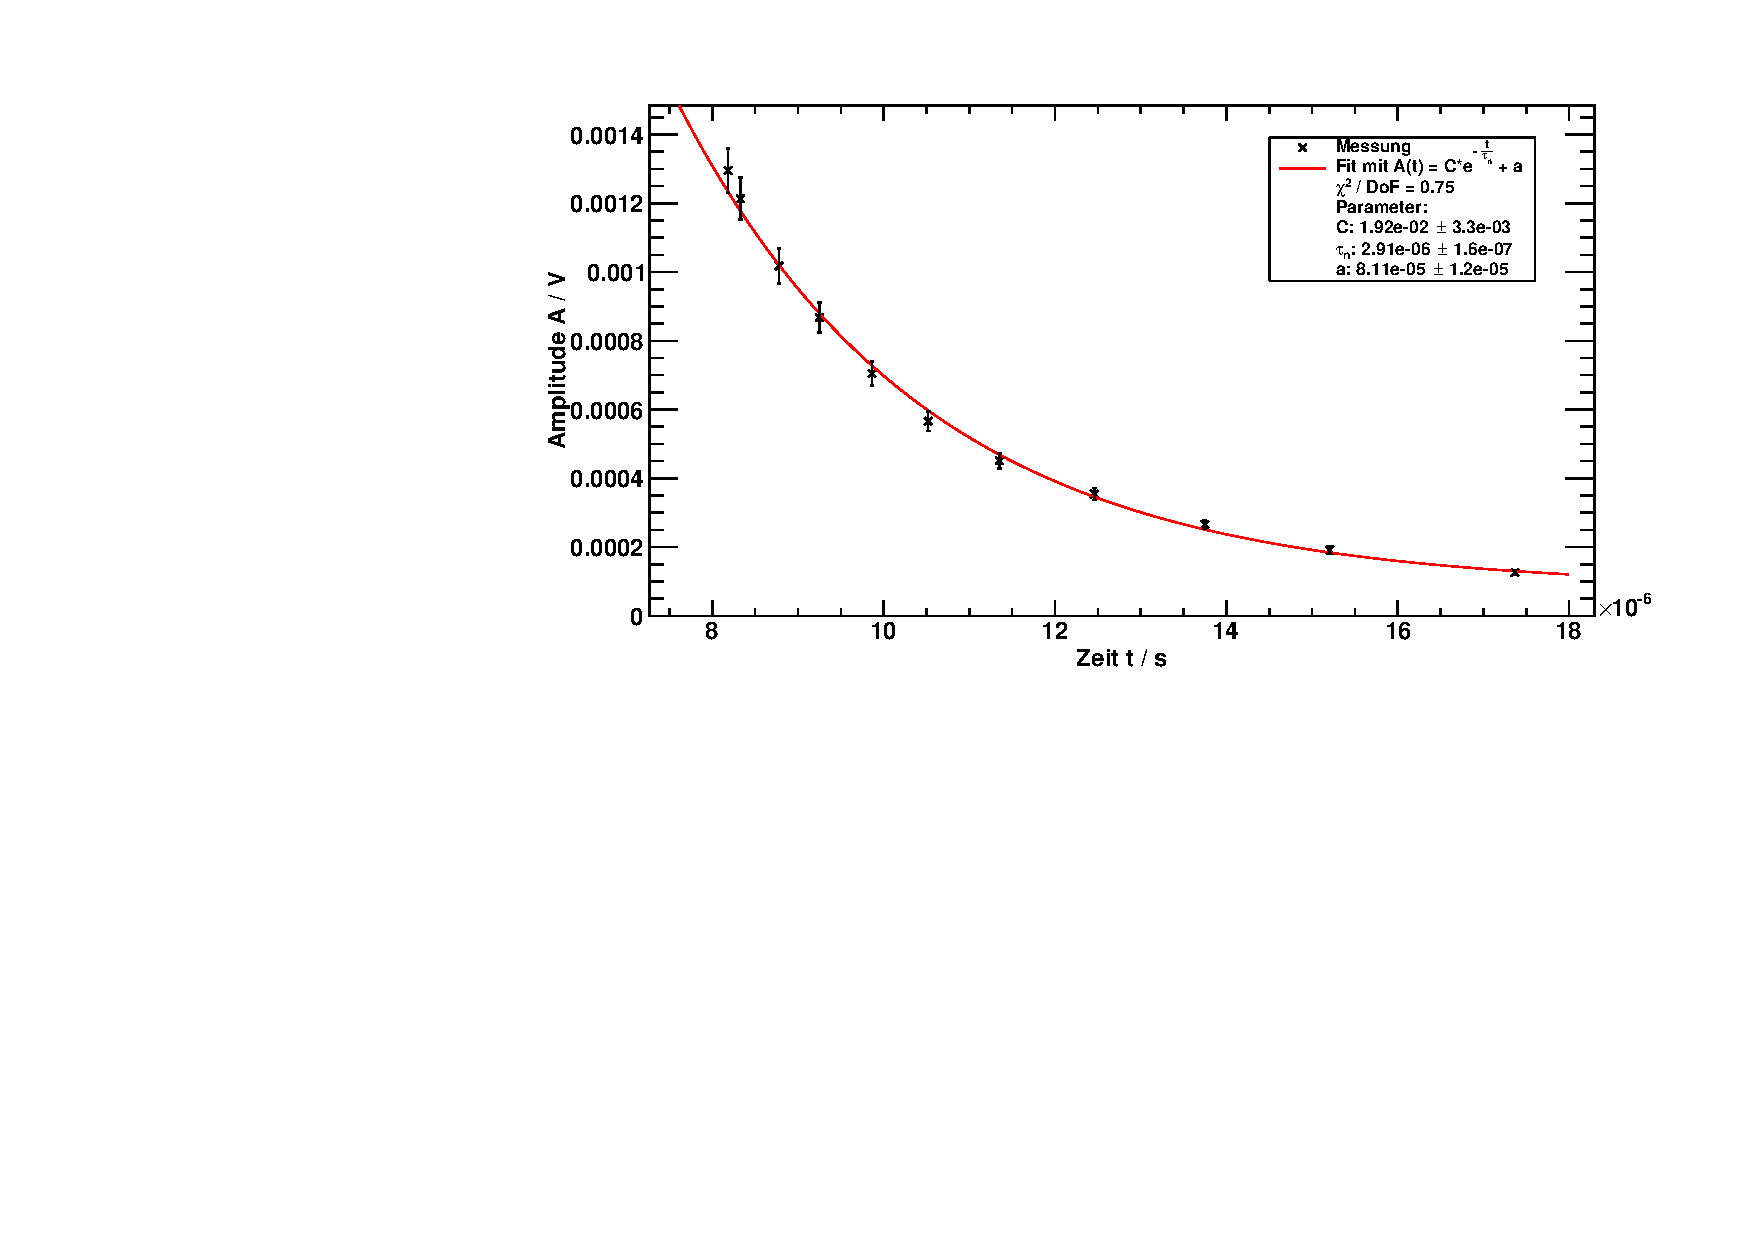
\includegraphics[width=\textwidth]{../img/part2/volt_fitA.pdf}
  \caption{caption}
  \label{img:volt:fita}
\end{center}
\end{figure}

\section{Halbleiterdetektoren}
\subsection{Versuchsaufbau}


\subsection{Versuchsdurchführung}
Mit zwei Halbleiterdetektoren aus Silizium und Cadmium-Tellurid werden die Spektren von Cobalt ($^{57}$Co)
und Americium ($^{241}$Am) untersucht. Die Messzeit beträgt für jede der vier Messungen 3600\,s.

\subsection{Messergebnisse und Auswertung}
Die Fehler der Counts $N$ sind poissonverteilt und betragen demnach $s_N = \sqrt{N}$. Sie sind in den Graphen der Spektren nicht eingezeichnet, 
da dies zu unübersichtlich ist. Bei den Fits der einzelnen Peaks sind die Fehler eingezeichnet, um die Übereinstimmung der gemessenen Werte 
mit dem theoretischen Modell zu visualisieren.
\subsubsection{CdTe-Detektor}
\paragraph{Spektren}
Die Spektren von \co\ und \am\ sind in \autoref{img:cdte:co:spektrum} und \autoref{img:cdte:am:spektrum} dargestellt. Man erkennt den 59.5\,keV-Peak 
von \am\, bei Kanal 300, den 122.06\,keV-Peak von \co\, bei Kanal 600 und den 136.47\,keV-Peak von \co\, bei Kanal 700.
\begin{figure}[H]
\begin{center}
  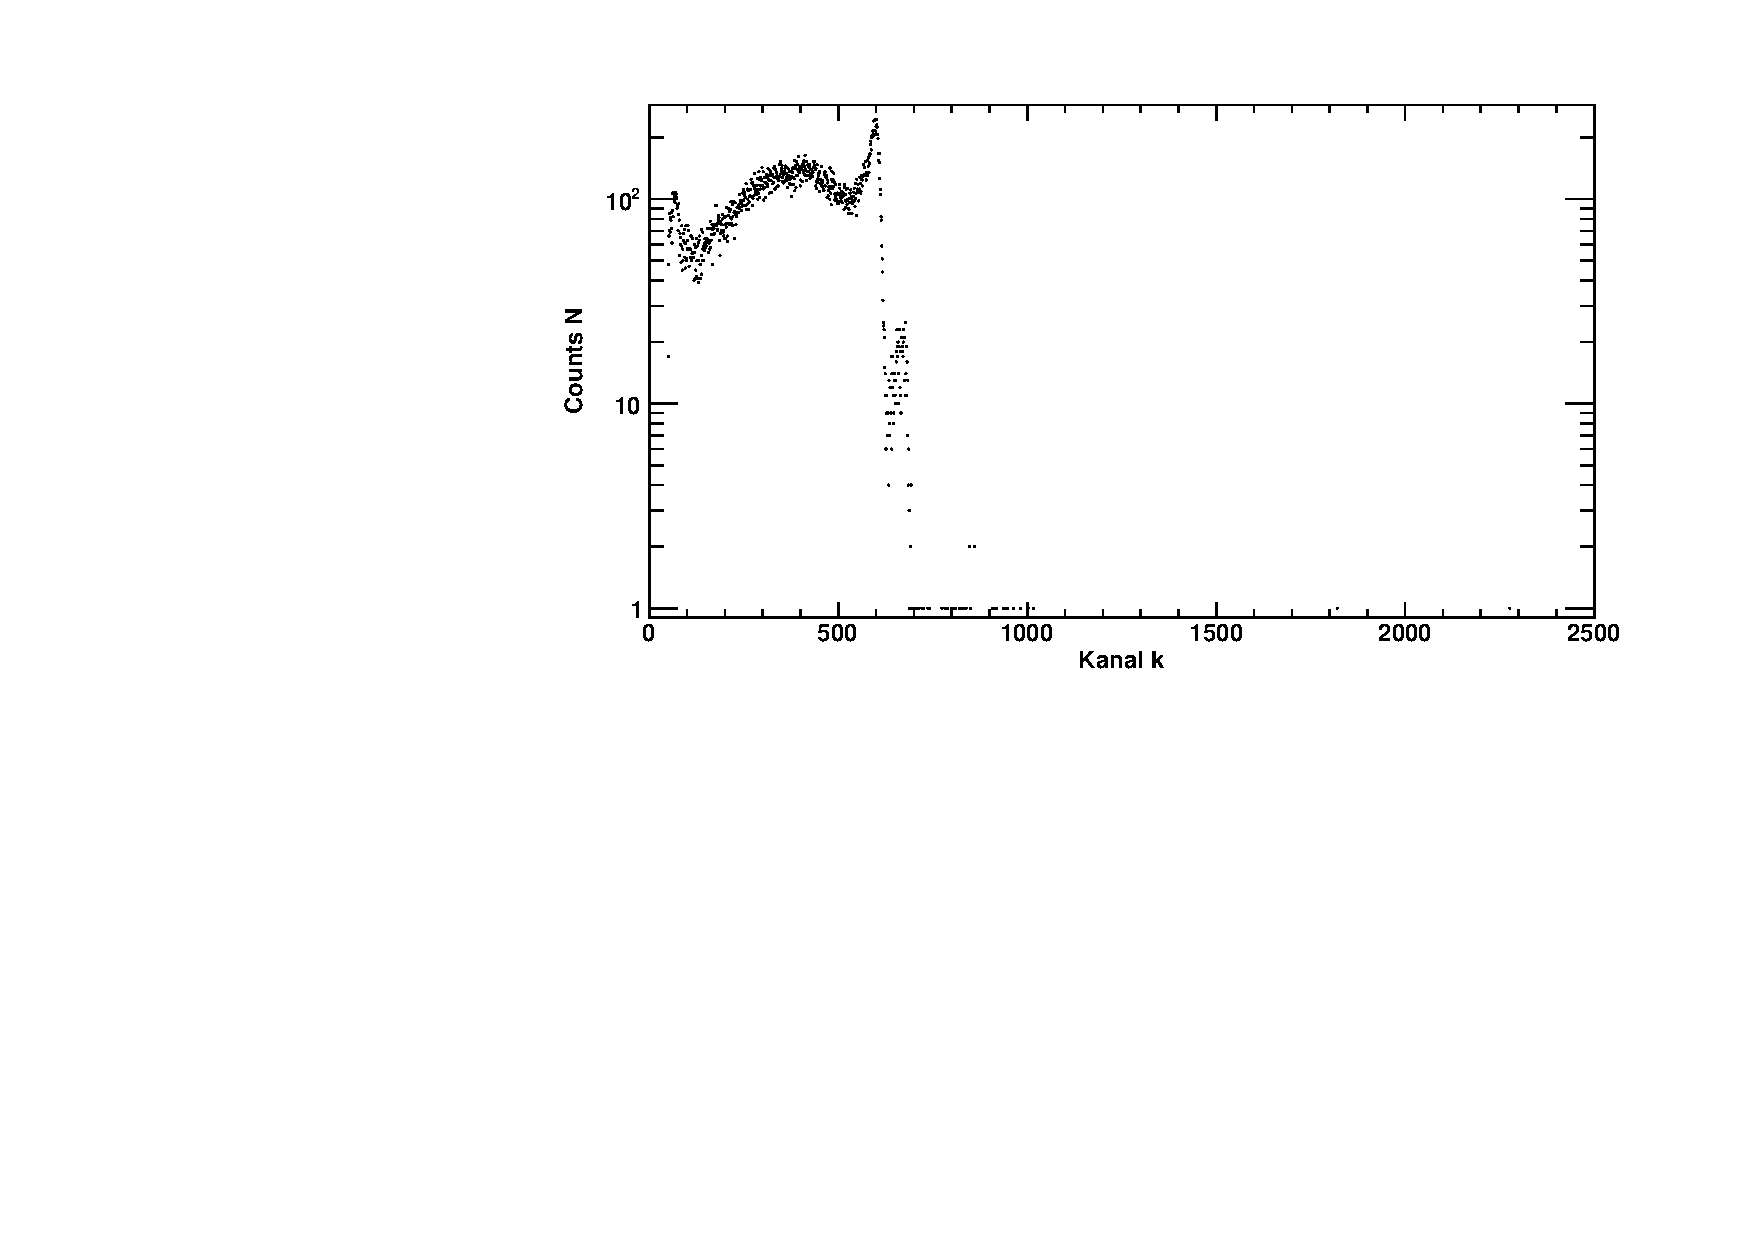
\includegraphics[width=0.95\textwidth]{../img/part3/Co-CdTe_spectrum.pdf}
  \caption{Spektrum von \co, gemessen mit dem CdTe-Detektor.}
  \label{img:cdte:co:spektrum}
\end{center}
\end{figure}

\begin{figure}[H]
\begin{center}
  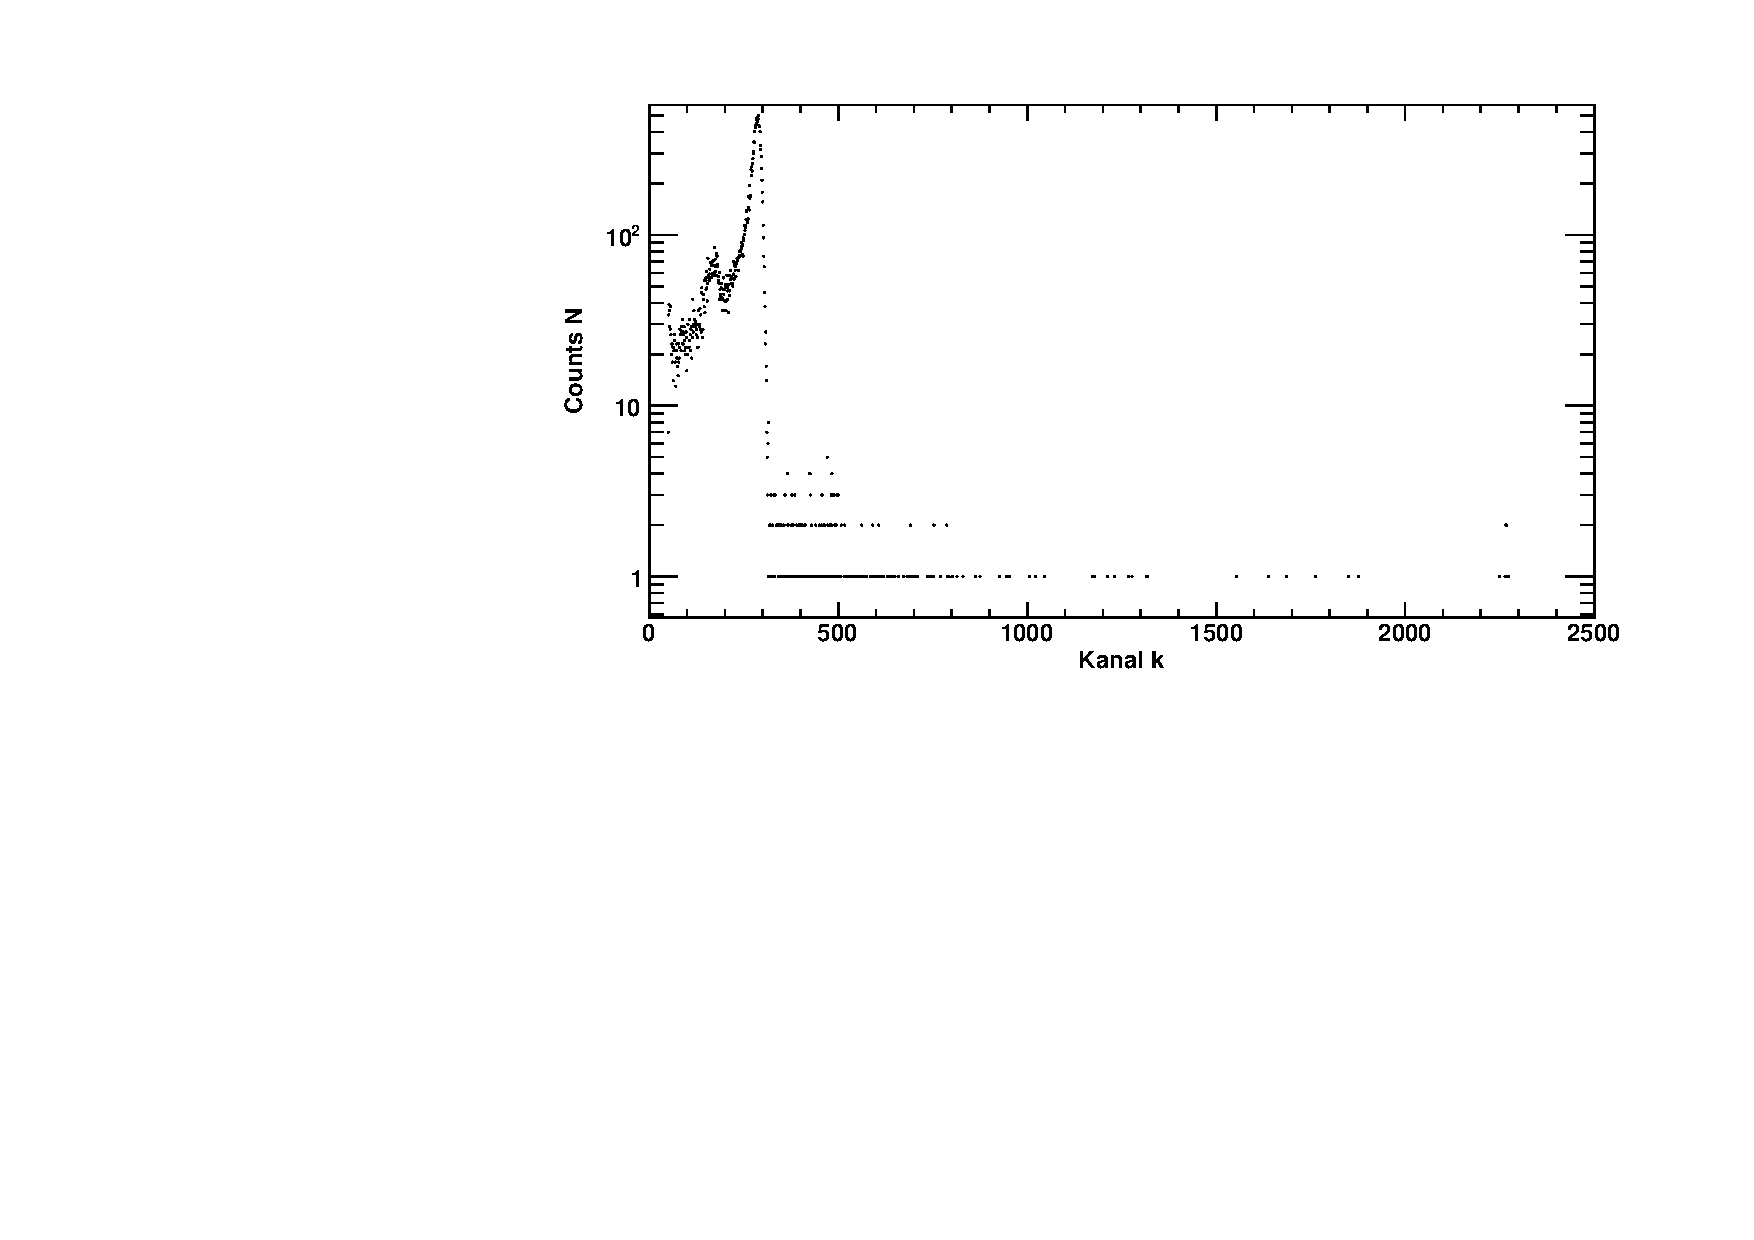
\includegraphics[width=0.95\textwidth]{../img/part3/Am-CdTe_spectrum.pdf}
  \caption{Spektrum von \am, gemessen mit dem CdTe-Detektor.}
  \label{img:cdte:am:spektrum}
\end{center}
\end{figure}


\paragraph{Peaks}
Die einzelnen Peaks werden mit einer normierten Gauß-Kurve gefittet.
\begin{equation}
  \label{eq:part3:normgauss}
  N(k) = A \cdot \frac{1}{\sqrt{2\pi \cdot \sigma^2}} \cdot e^{-\frac{1}{2} \left( \frac{k-k_c}{\sigma} \right)^2}
\end{equation}
Die Fits sind in \autoref{img:am:cdte:peak0}, \autoref{img:co:cdte:peak0} und \autoref{img:co:cdte:peak1} dargestellt. Wie man erkennt, sind die 
Peaks nicht ganz symmetrisch.
Durch die unterschiedliche Absorptionstiefe ist der Abstand zu Kathode und Anode nicht konstant, die 
entstandenen Ladungsträger rekombinieren teilweise wieder. Dieser Effekt soll jedoch nach \cite{staatsex} nicht berücksichtigt werden, die 
Peaks können in guter Näherung mit einer Gauß-Kurve gefittet werden.
\begin{figure}[H]
\begin{center}
  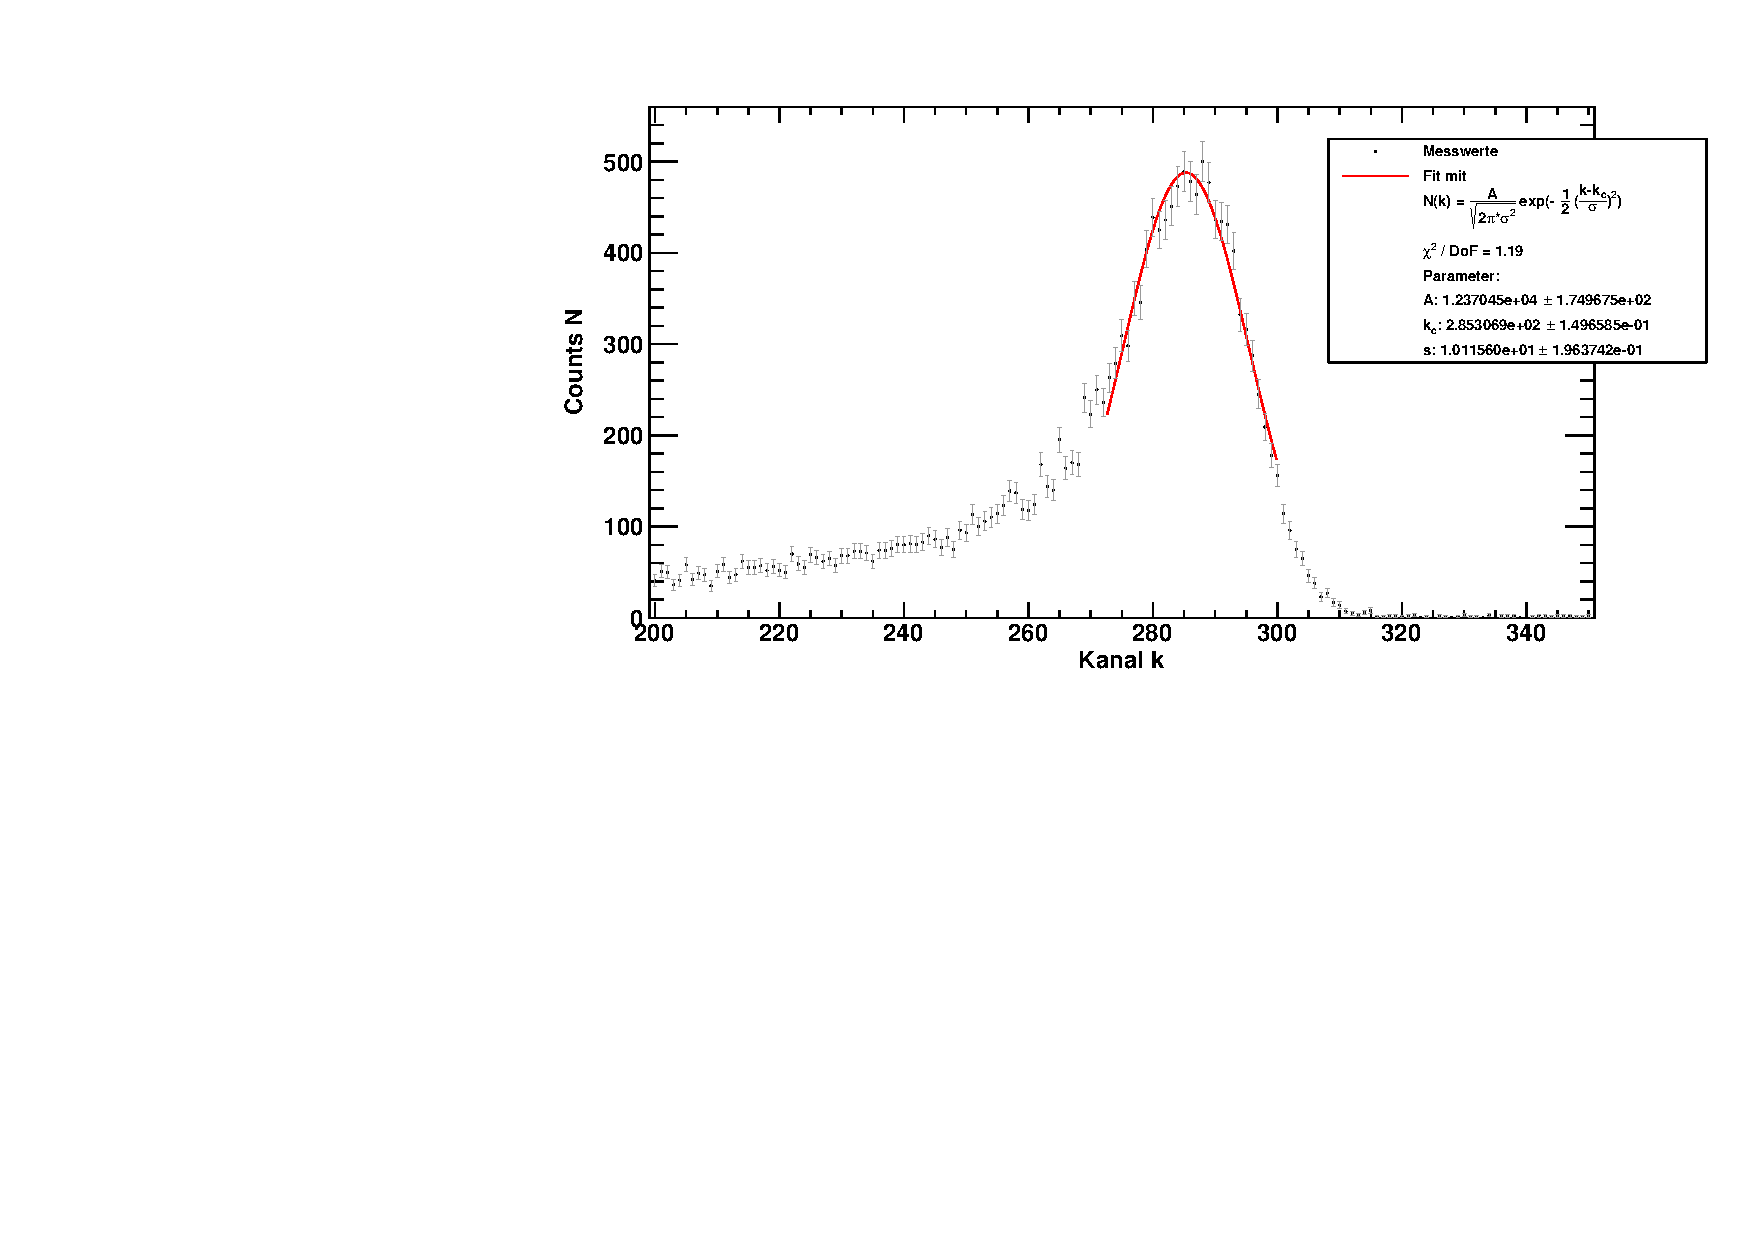
\includegraphics[width=\textwidth]{../img/part3/Am-CdTe_00.pdf}
  \caption{59.5\,keV-Peak von \am, gemessen mit dem CdTe-Detektor.}
  \label{img:am:cdte:peak0}
\end{center}
\end{figure}

\begin{figure}[H]
\begin{center}
  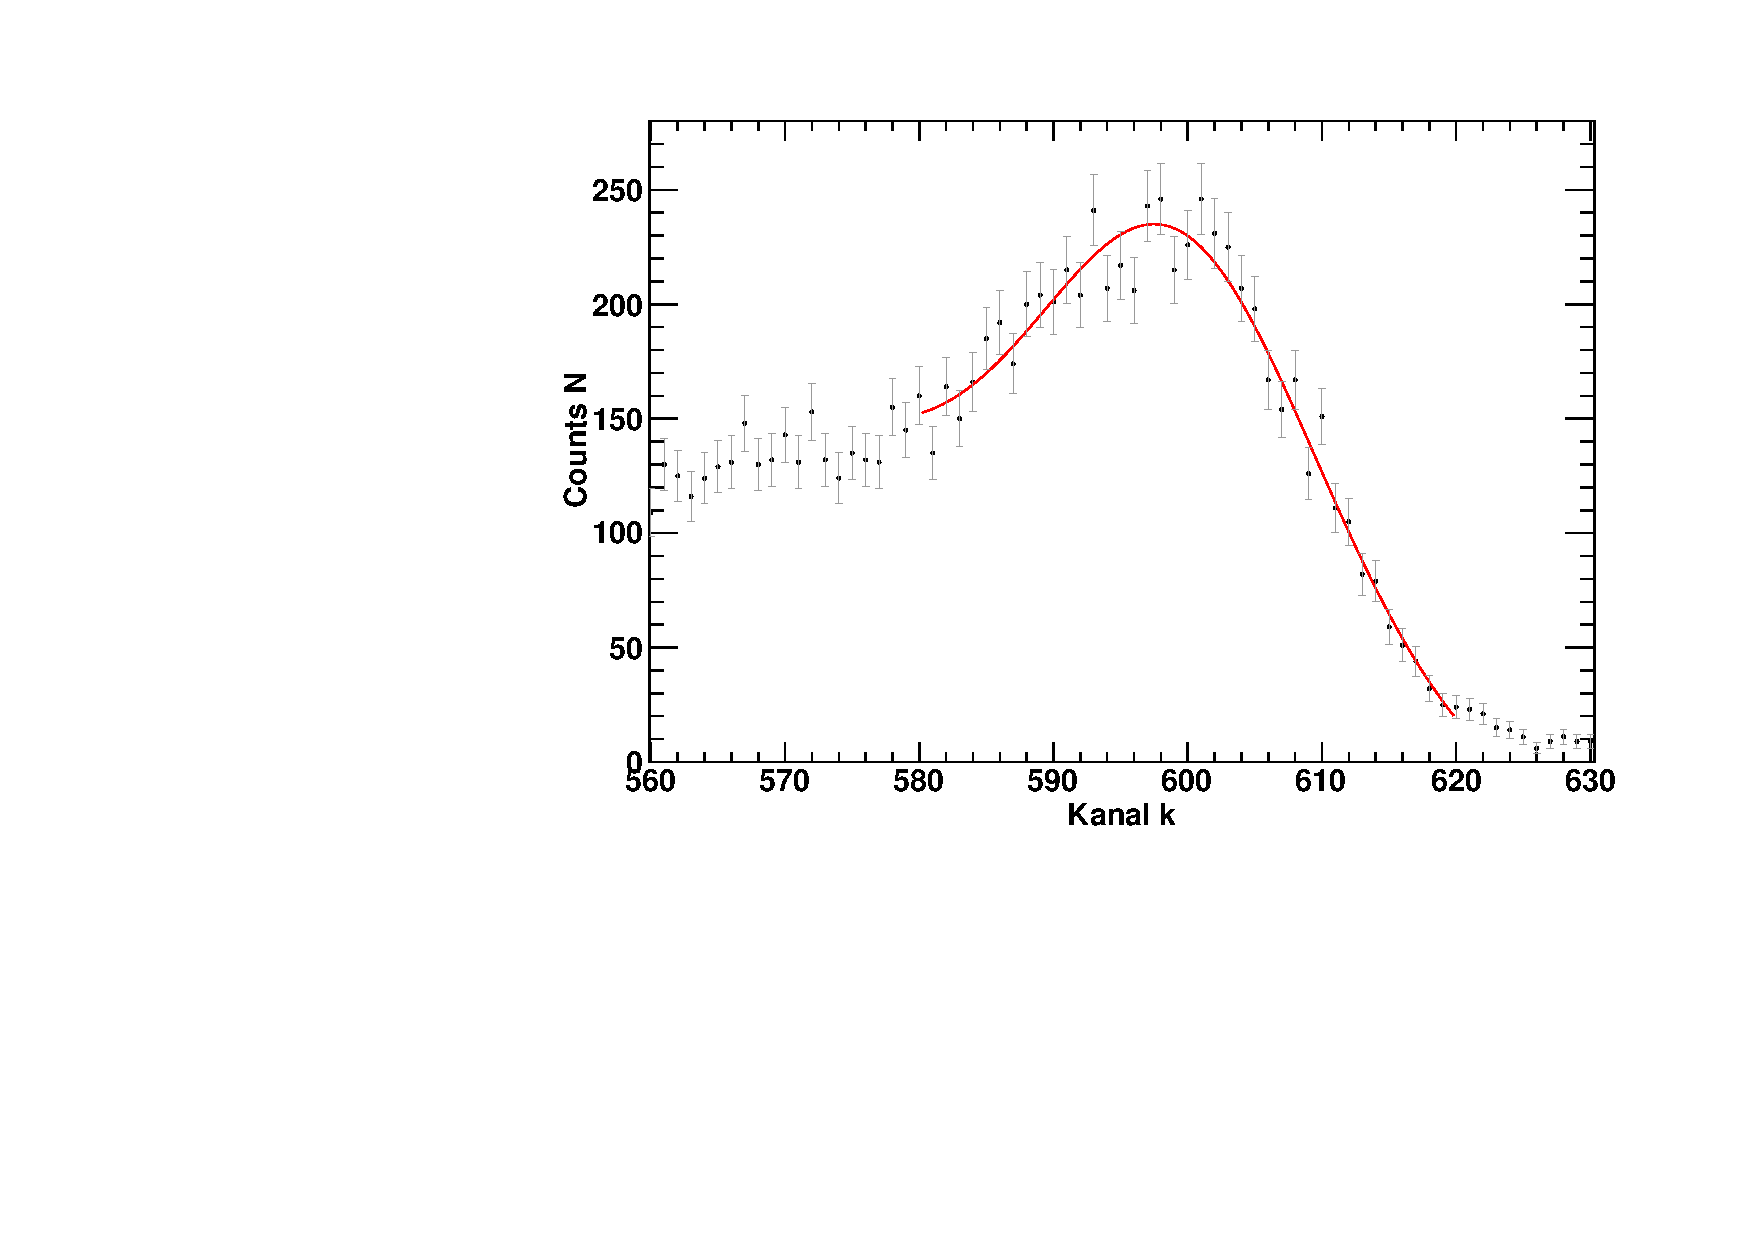
\includegraphics[width=\textwidth]{../img/part3/Co-CdTe_00.pdf}
  \caption{122.06\,keV-Peak von \co, gemessen mit dem CdTe-Detektor.}
  \label{img:co:cdte:peak0}
\end{center}
\end{figure}

\begin{figure}[H]
\begin{center}
  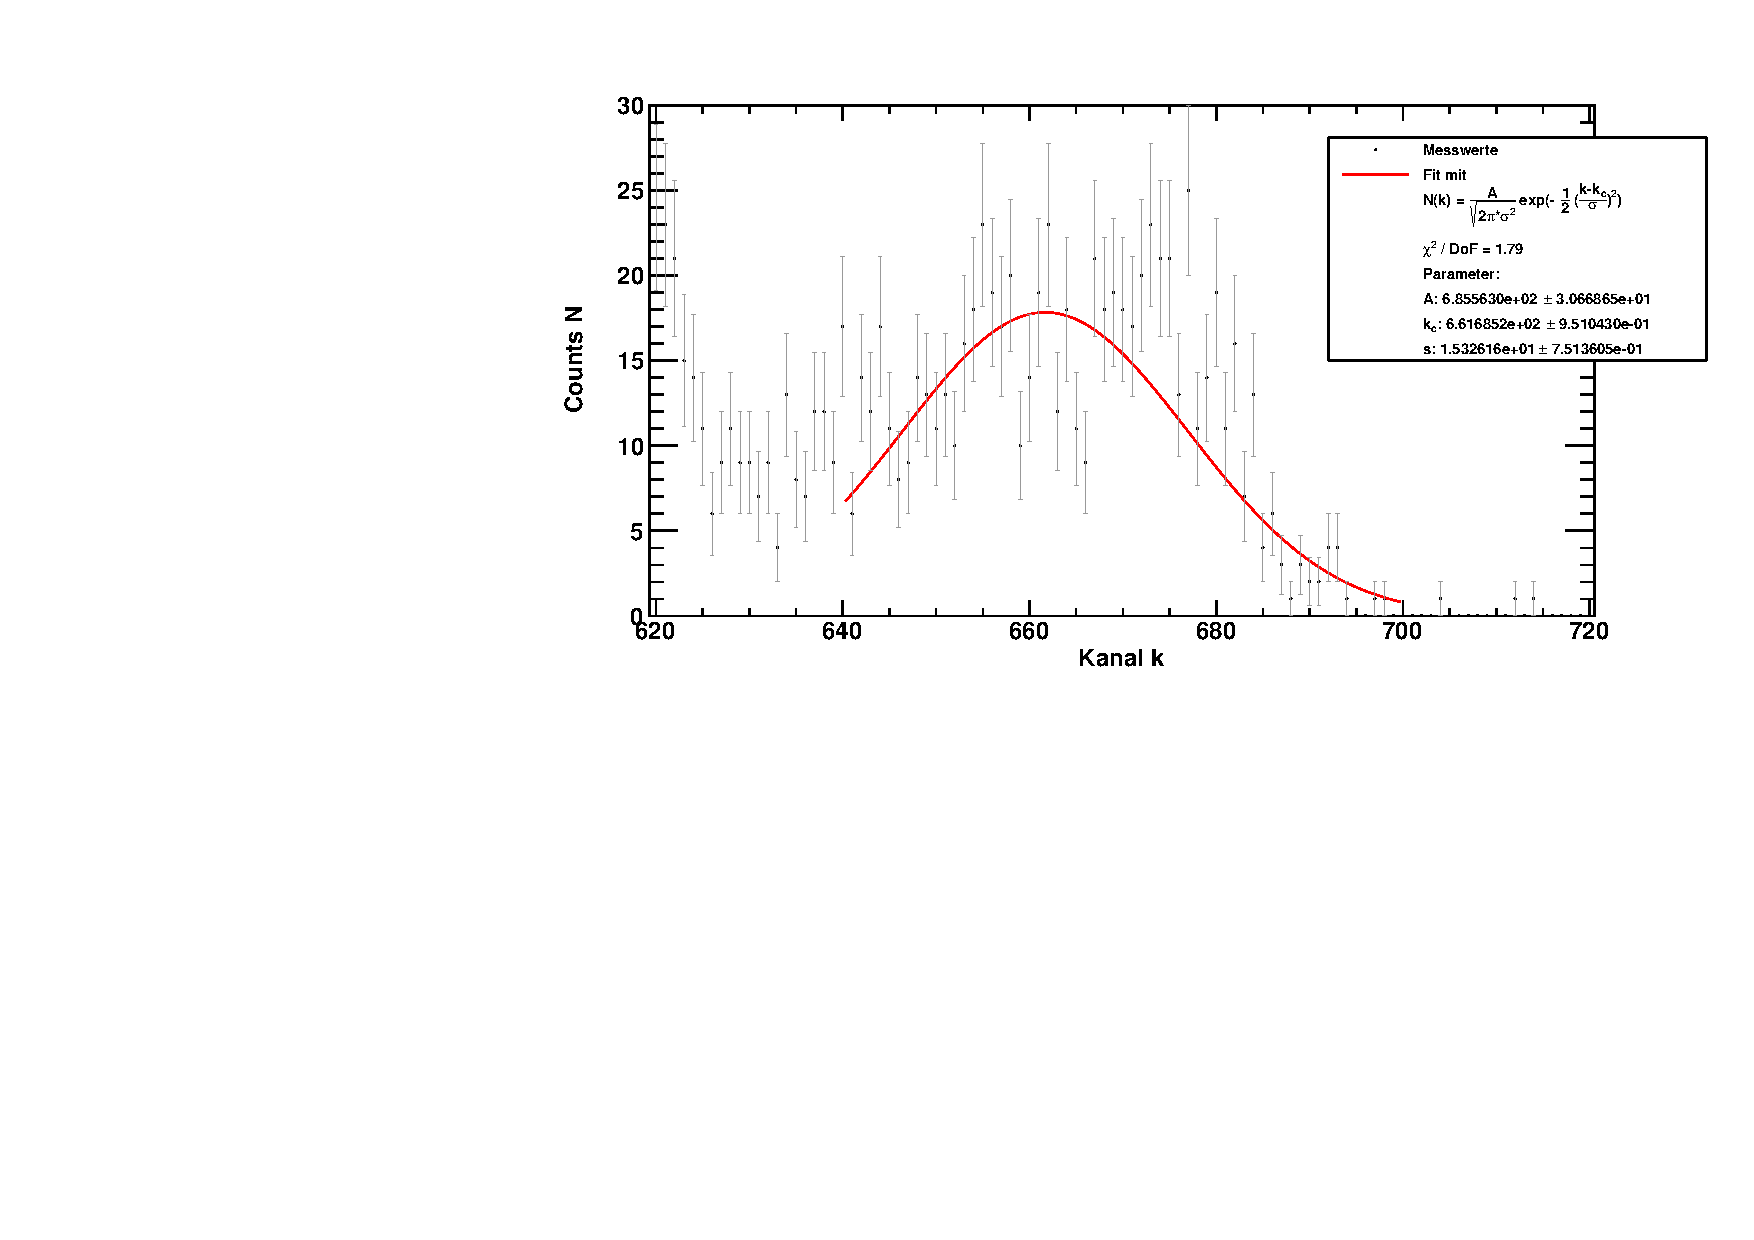
\includegraphics[width=\textwidth]{../img/part3/Co-CdTe_01.pdf}
  \caption{136.47\,keV-Peak von \co, gemessen mit dem CdTe-Detektor.}
  \label{img:co:cdte:peak1}
\end{center}
\end{figure}

\paragraph{Energieeichung}
Die Literaturwerte der Peaks werden über den oben erhaltenen Erwartungswerten der Gauß-Kurven aufgetragen. Dieser Graph ist Grundlage der 
Energieeichung (\autoref{img:cdte:energygauge}). Es wird eine lineare Abhängigkeit der gemessenen Energie $E$ von der Kanalnummer $k$ angenommen.
\begin{equation}
  E(k) = a + b \cdot k
\end{equation}
Man erhält für die Parameter:
\begin{equation}
\begin{split}
  a &= (1.86 \pm 0.09)\,\text{eV} \\
  b &= (0.2020 \pm 0.0003)\,\text{eV}
\end{split}
\end{equation}
\begin{figure}[H]
\begin{center}
  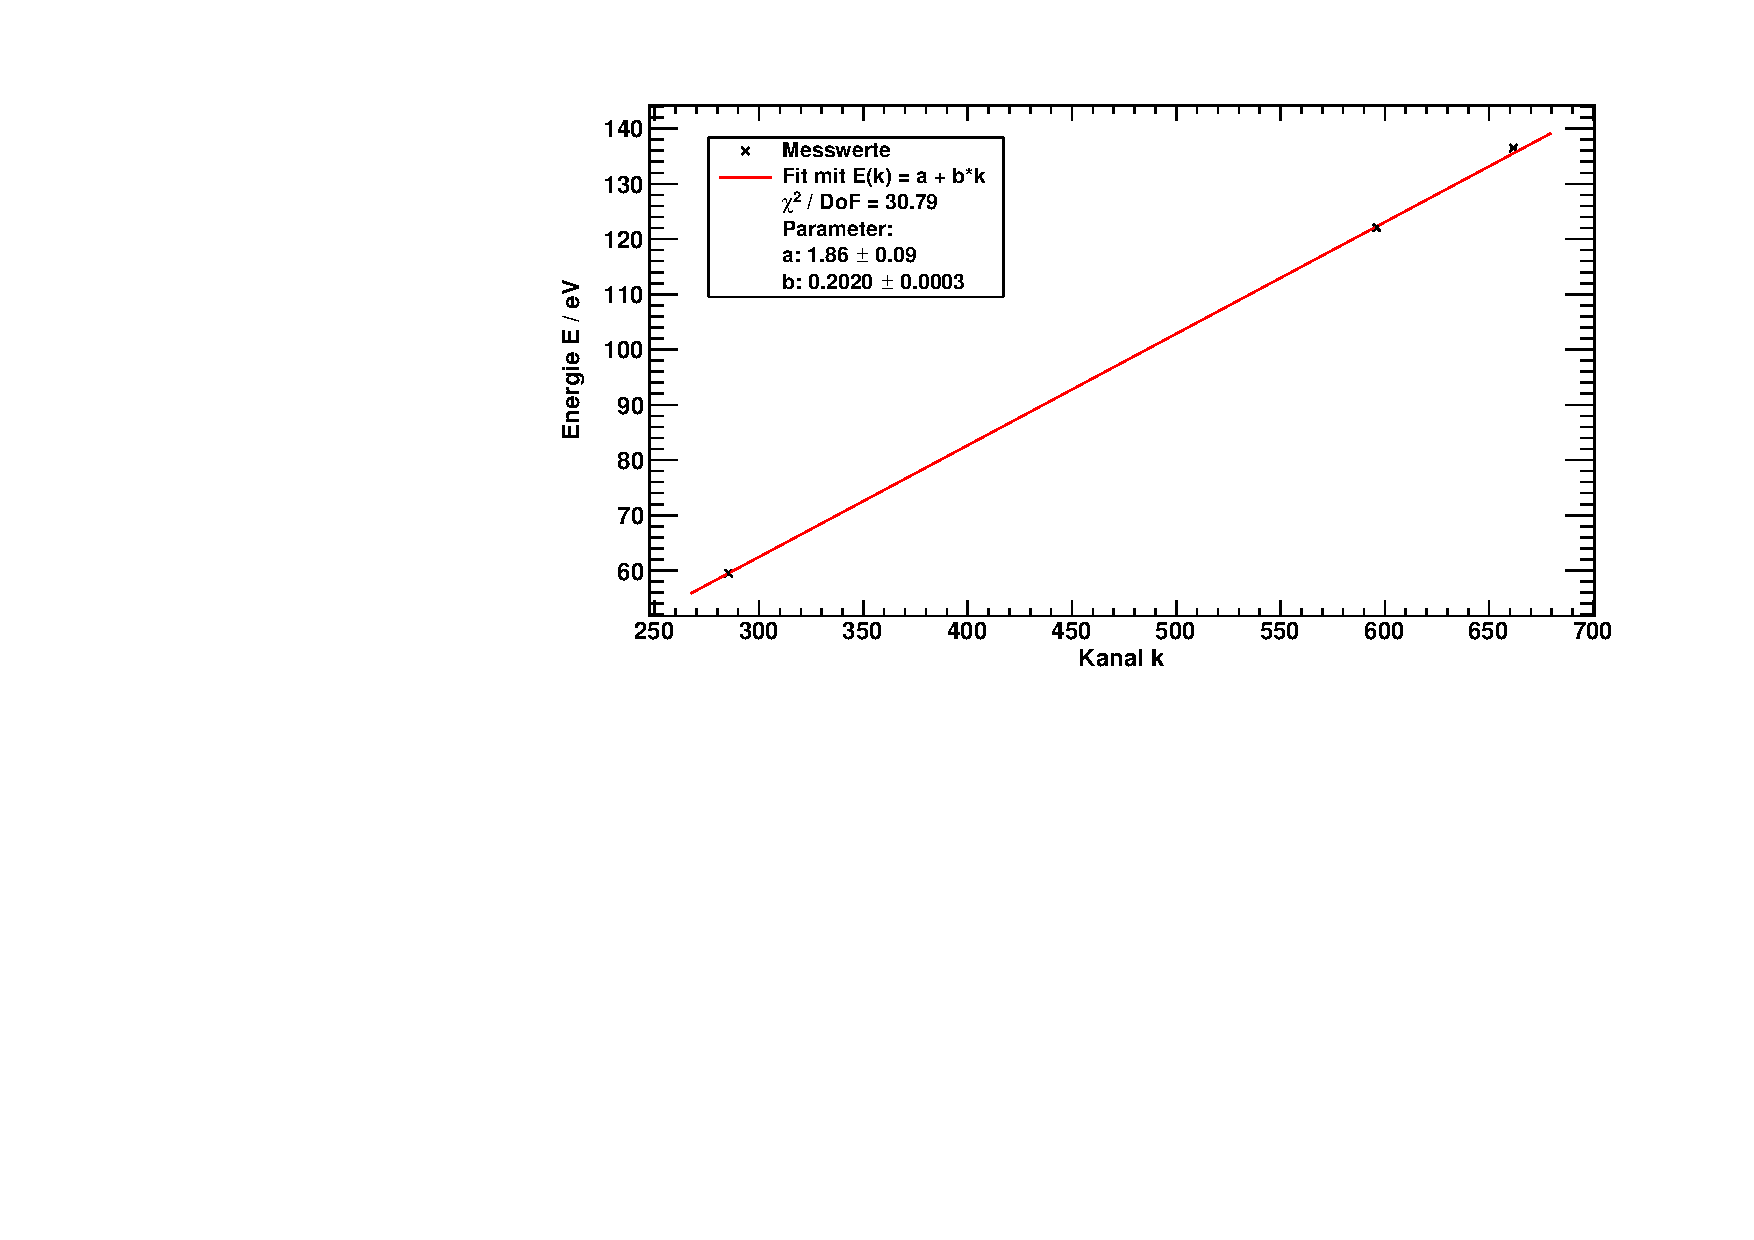
\includegraphics[width=\textwidth]{../img/part3/energygauge_CdTe.pdf}
  \caption{Energieeichung des CdTe-Detektors.}
  \label{img:cdte:energygauge}
\end{center}
\end{figure}
Der hohe Wert des $\chi^2$ kann mit einer Nichtlinearität des Detektors oder des MCA erklärt werden. Allerdings ist ein quadratischer Fit 
(vermutetes Modell) bei nur drei Messpunkten nicht sinnvoll, da die Anzahl der einzelnen Messpunkte der Anzahl der Fitparameter entspricht, es 
gibt dann keinen Freiheitsgrad.
Die Fehler der Messpunkte stammen aus den Fits (die akzeptable $\chi^2$-Werte besitzen). Die Counts 
wurden wie oben beschrieben als poissonverteilt angenommen.

\paragraph{Relative Energieauflösung}
Die relativen Energieauflösungen wurden aus der Position $k_c$ und der Standardabweichung bestimmt (\autoref{tab:cdte:rer}). 
\begin{equation}
  \label{eq:rer}
  \text{RER} = \frac{2 \sqrt{2 \ln(2)} \cdot \sigma}{k_c} 
\end{equation}
\begin{table}[H]
\begin{center}
\begin{tabular}{|c|c|}
\hline 
Kanal & RER \\ \hline
285.31 $\pm$ 0.15 & 0.0835 $\pm$ 0.0016\\ \hline
596.1 $\pm$ 0.4 & 0.055 $\pm$ 0.003 \\ \hline
661.7 $\pm$ 1.0 & 0.055 $\pm$ 0.003 \\ \hline
\end{tabular}
\caption{Energieauflösungen des CdTe-Detektors}
\label{tab:cdte:rer}
\end{center}
\end{table}

\subsubsection{Si-Detektor}
\paragraph{Spektren}
In den Spektren von \co\ und \am\ (\autoref{img:si:co:spektrum} und \autoref{img:si:am:spektrum}) sieht den 59.5\,keV-Peak 
von \am\, bei Kanal 300 und den 122.06\,keV-Peak von \co\, bei Kanal 600. Der 136.47\,keV-Peak von \co\, lässt sich im Gesamtspektrum 
ohne Vergrößerung (der x-Achse) nicht mehr erkennen, er lässt sich allerdings direkt rechts neben dem 122.06\,keV-Peak finden.
\begin{figure}[H]
\begin{center}
  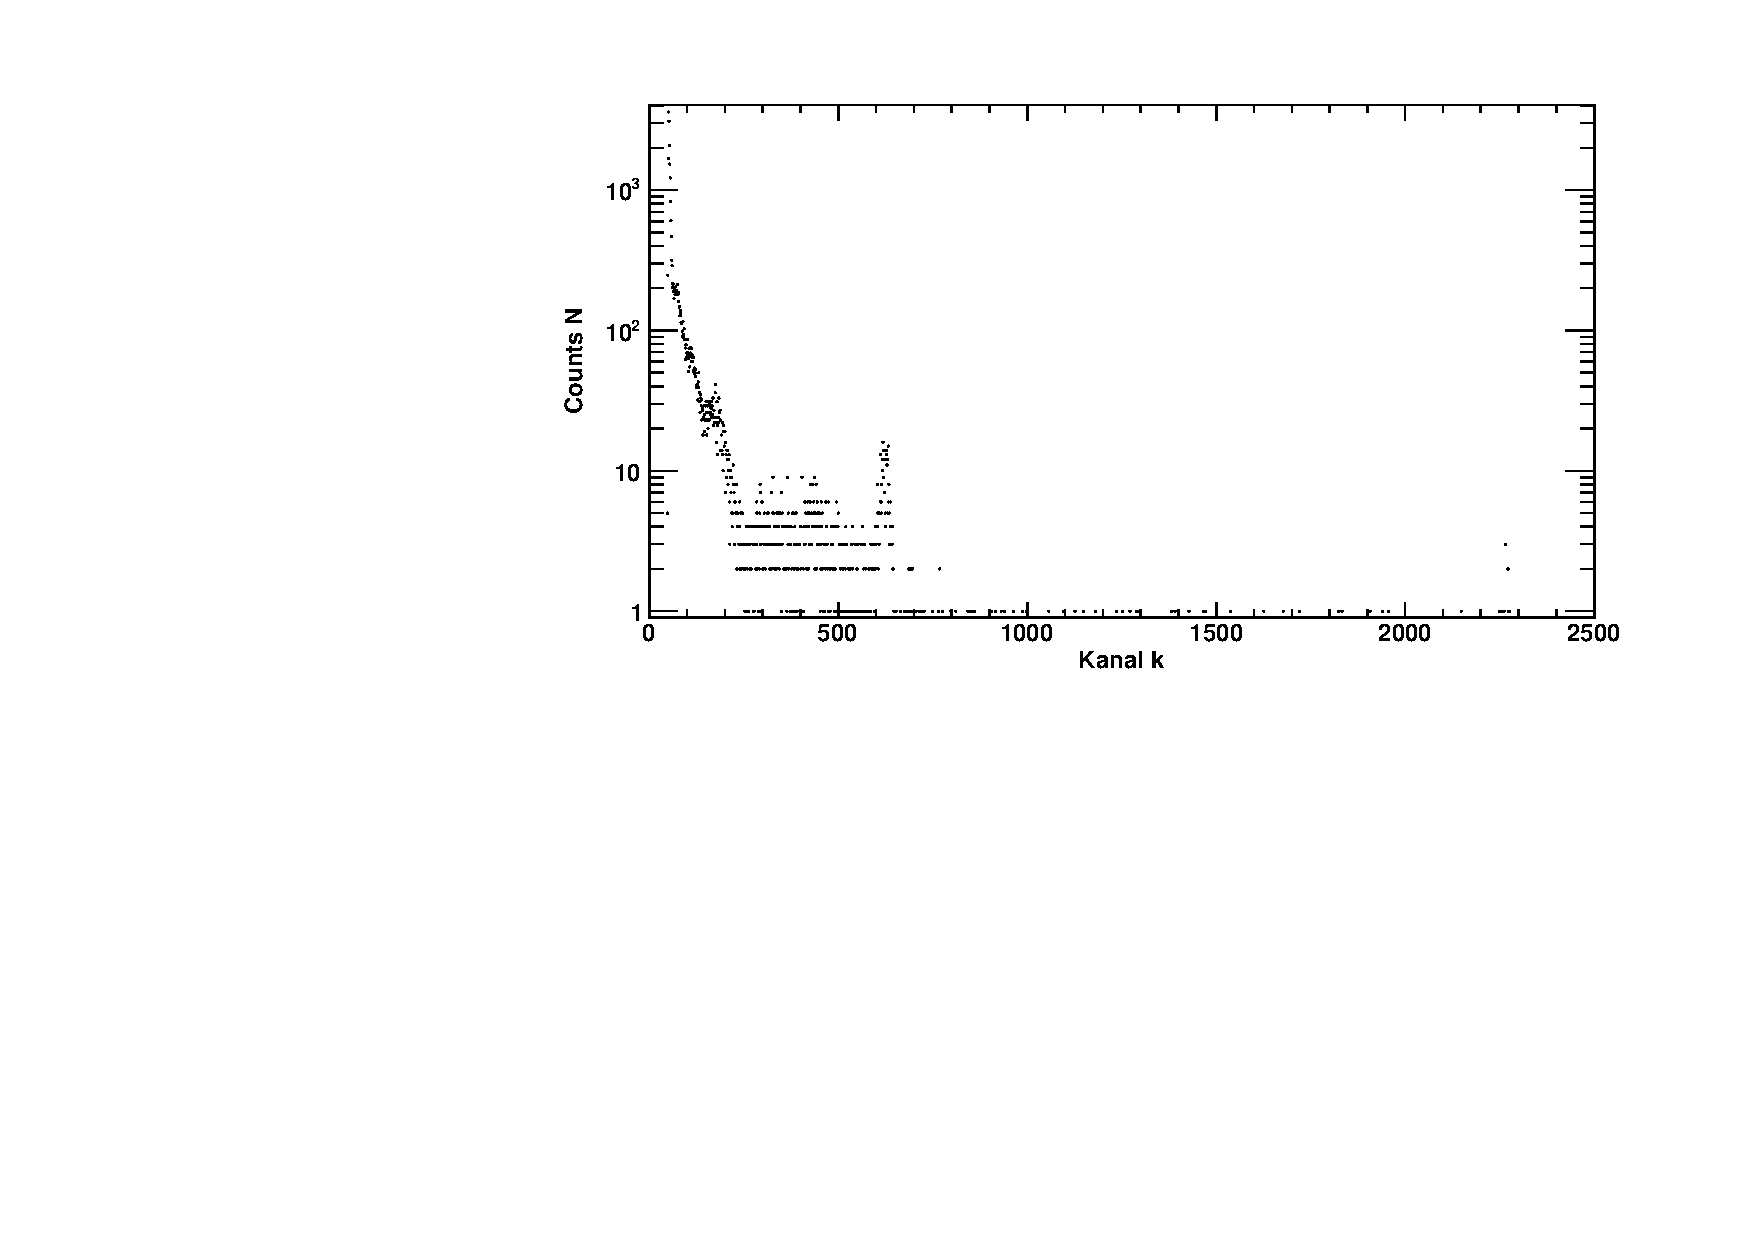
\includegraphics[width=\textwidth]{../img/part3/Co-Si_spectrum.pdf}
  \caption{Spektrum von \co, gemessen mit dem Si-Detektor.}
  \label{img:si:co:spektrum}
\end{center}
\end{figure}

\begin{figure}[H]
\begin{center}
  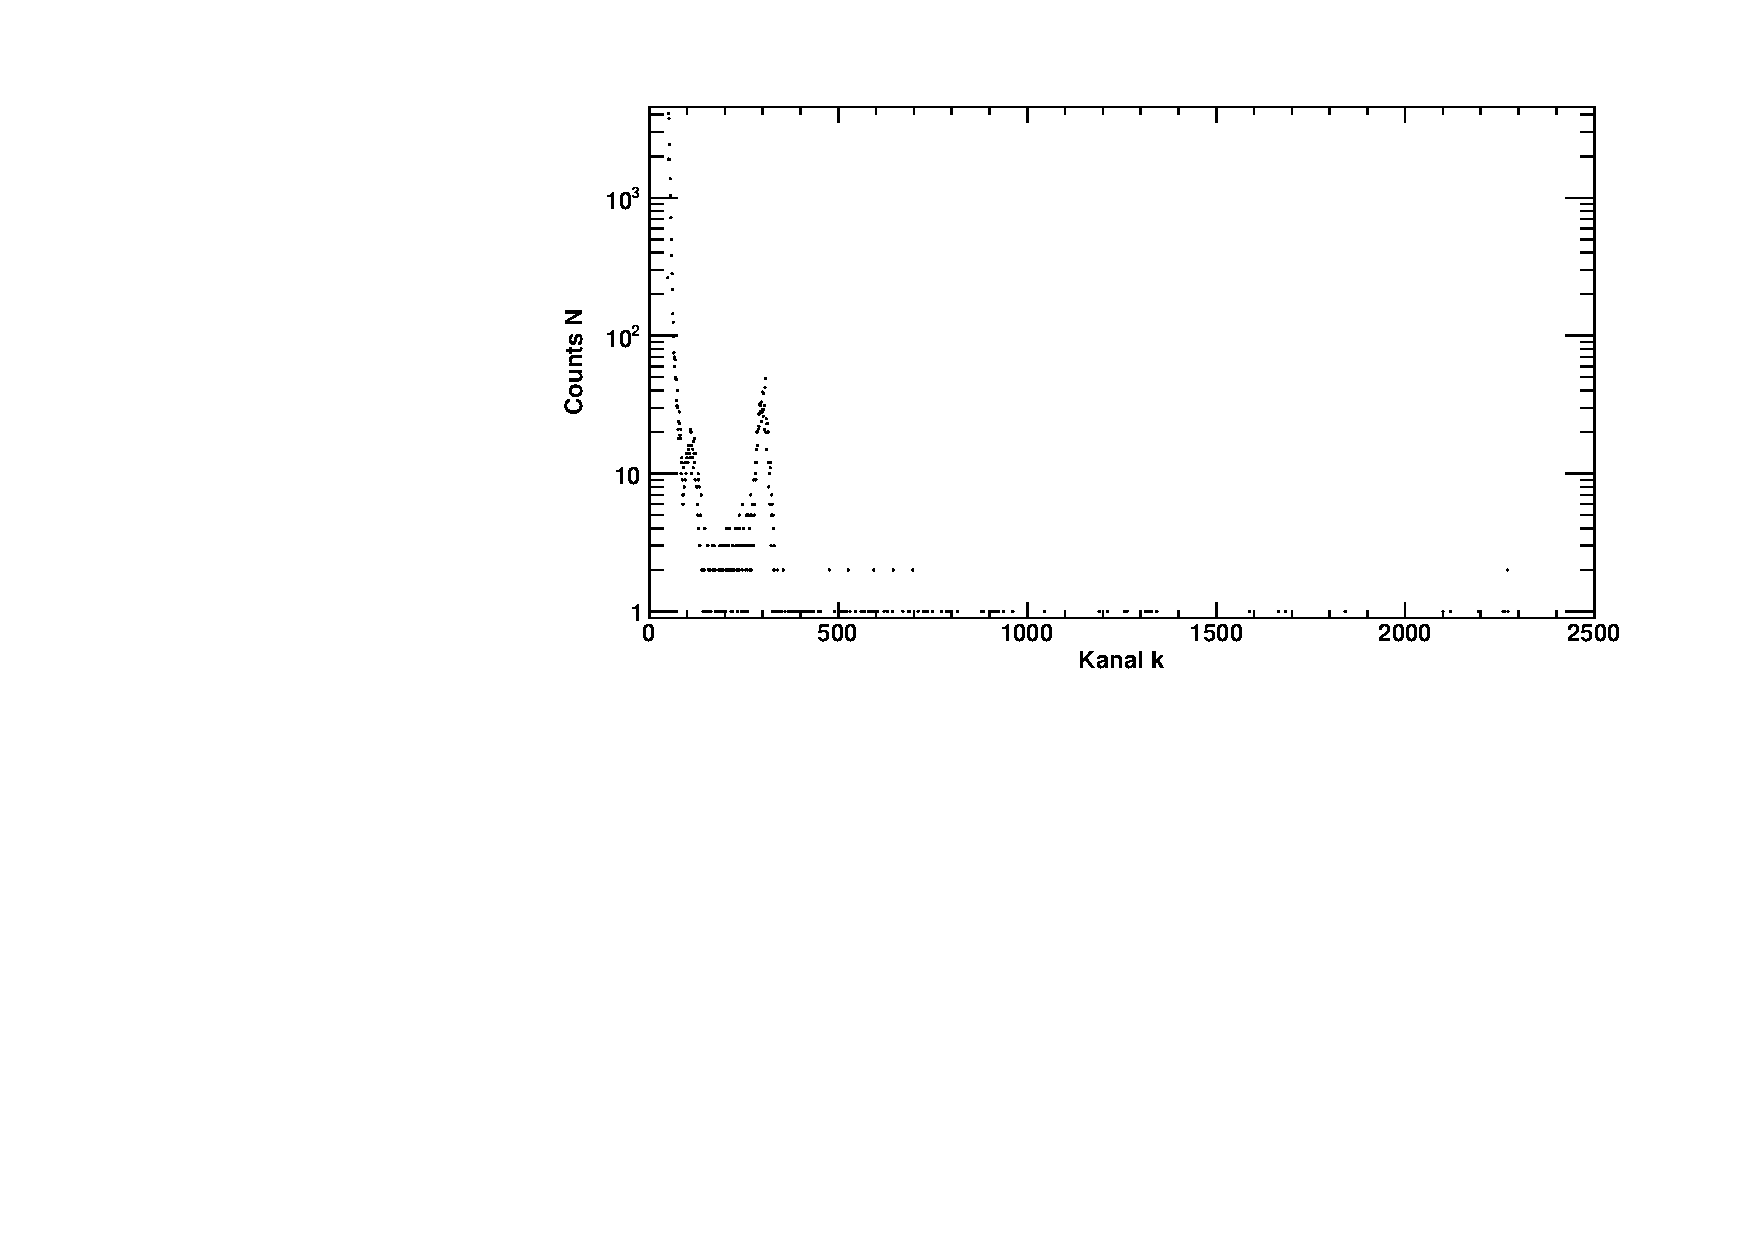
\includegraphics[width=\textwidth]{../img/part3/Am-Si_spectrum.pdf}
  \caption{Spektrum von \am, gemessen mit dem Si-Detektor.}
  \label{img:si:am:spektrum}
\end{center}
\end{figure}

\paragraph{Peaks}
Die Peaks werden wieder mit der normierten Gaußkurve (\autoref{eq:part3:normgauss}) gefittet 
(\autoref{img:am:si:peak0}, \autoref{img:co:si:peak0} und \autoref{img:co:si:peak1}). Jedoch hat der 136.47\,keV-Peak von \co\ eine zu kleine 
Anzahl von Counts, dass man noch gut eine Gaußkurve erkennen und anpassen kann. Im nächsten Abschnitt wird erklärt, wie man doch noch 
Informationen über die Lage und Ausdehnung des Peaks erhalten kann.
\begin{figure}[H]
\begin{center}
  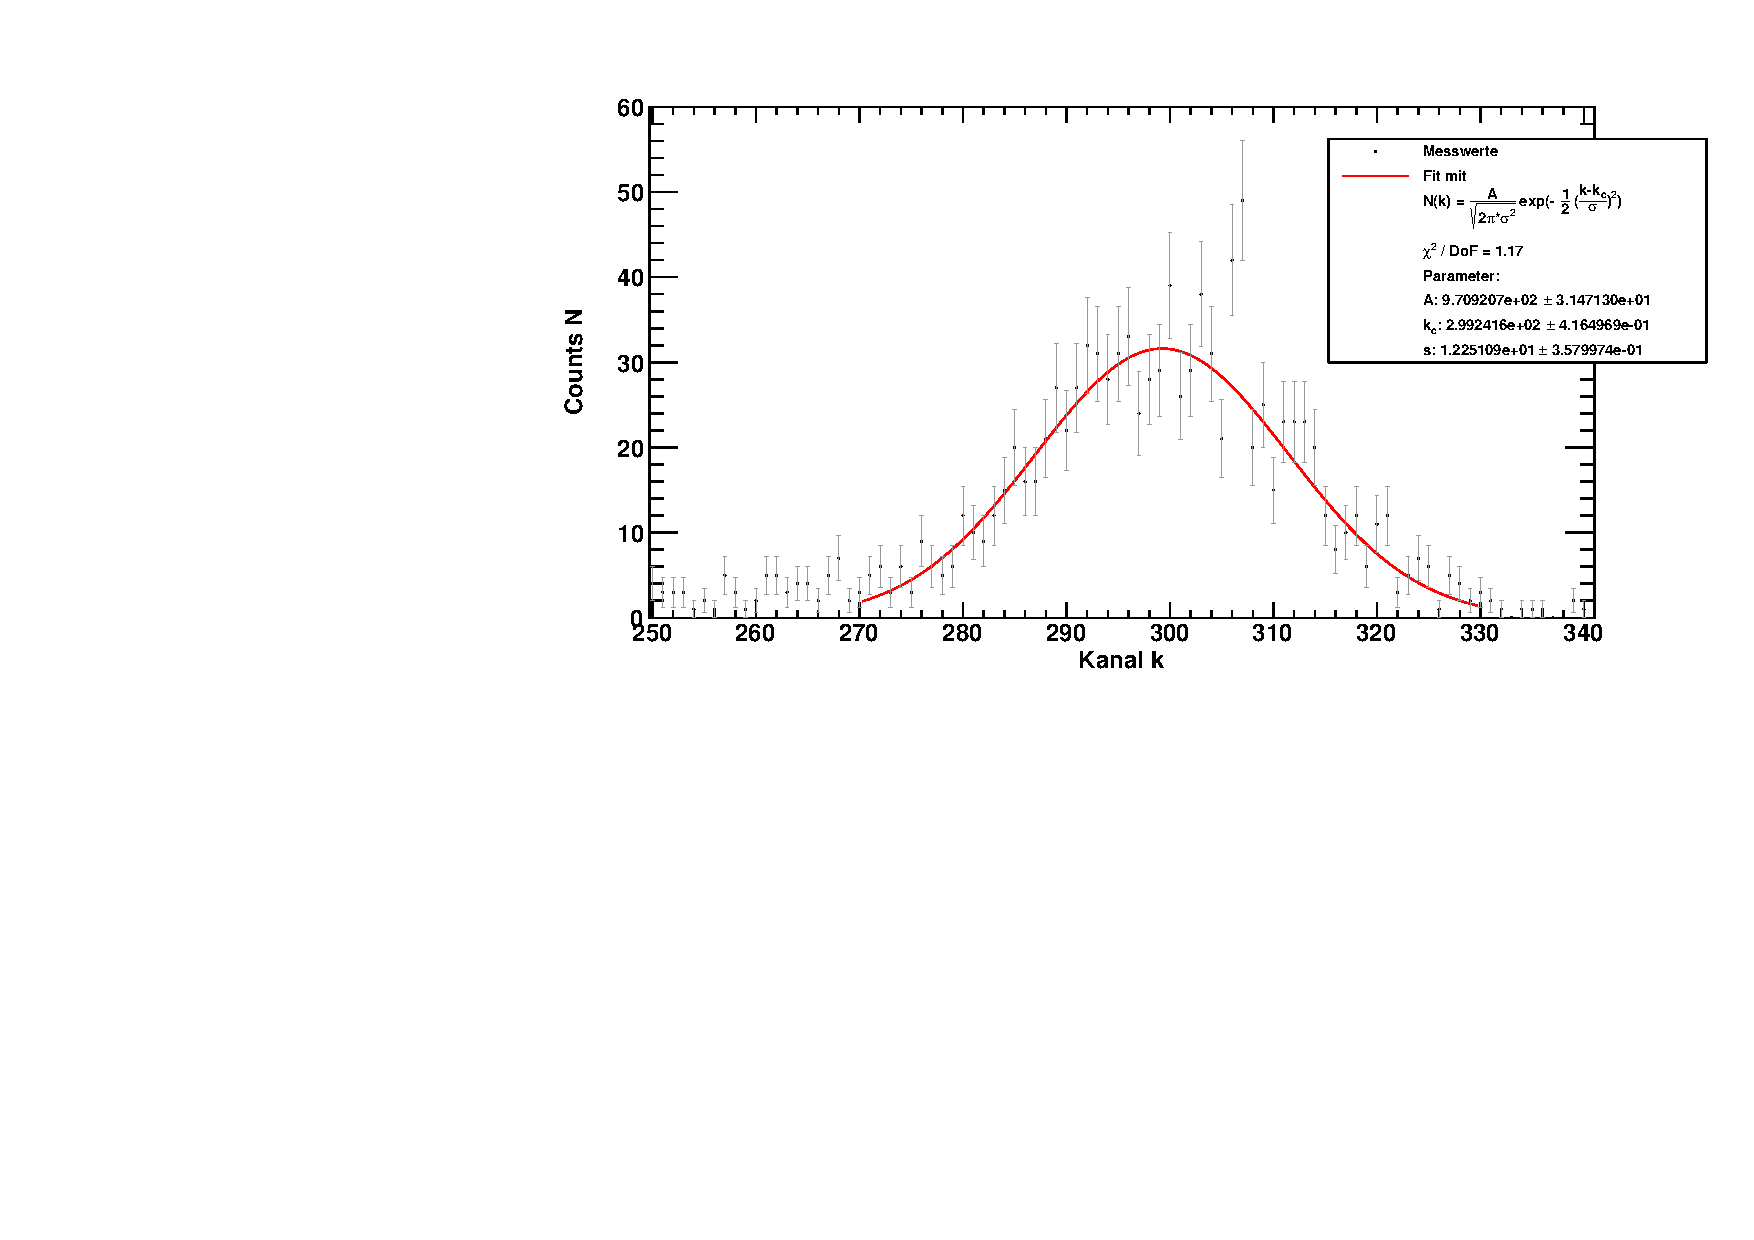
\includegraphics[width=\textwidth]{../img/part3/Am-Si_00.pdf}
  \caption{59.5\,keV-Peak von \am, gemessen mit dem Si-Detektor.}
  \label{img:am:si:peak0}
\end{center}
\end{figure}

\begin{figure}[H]
\begin{center}
  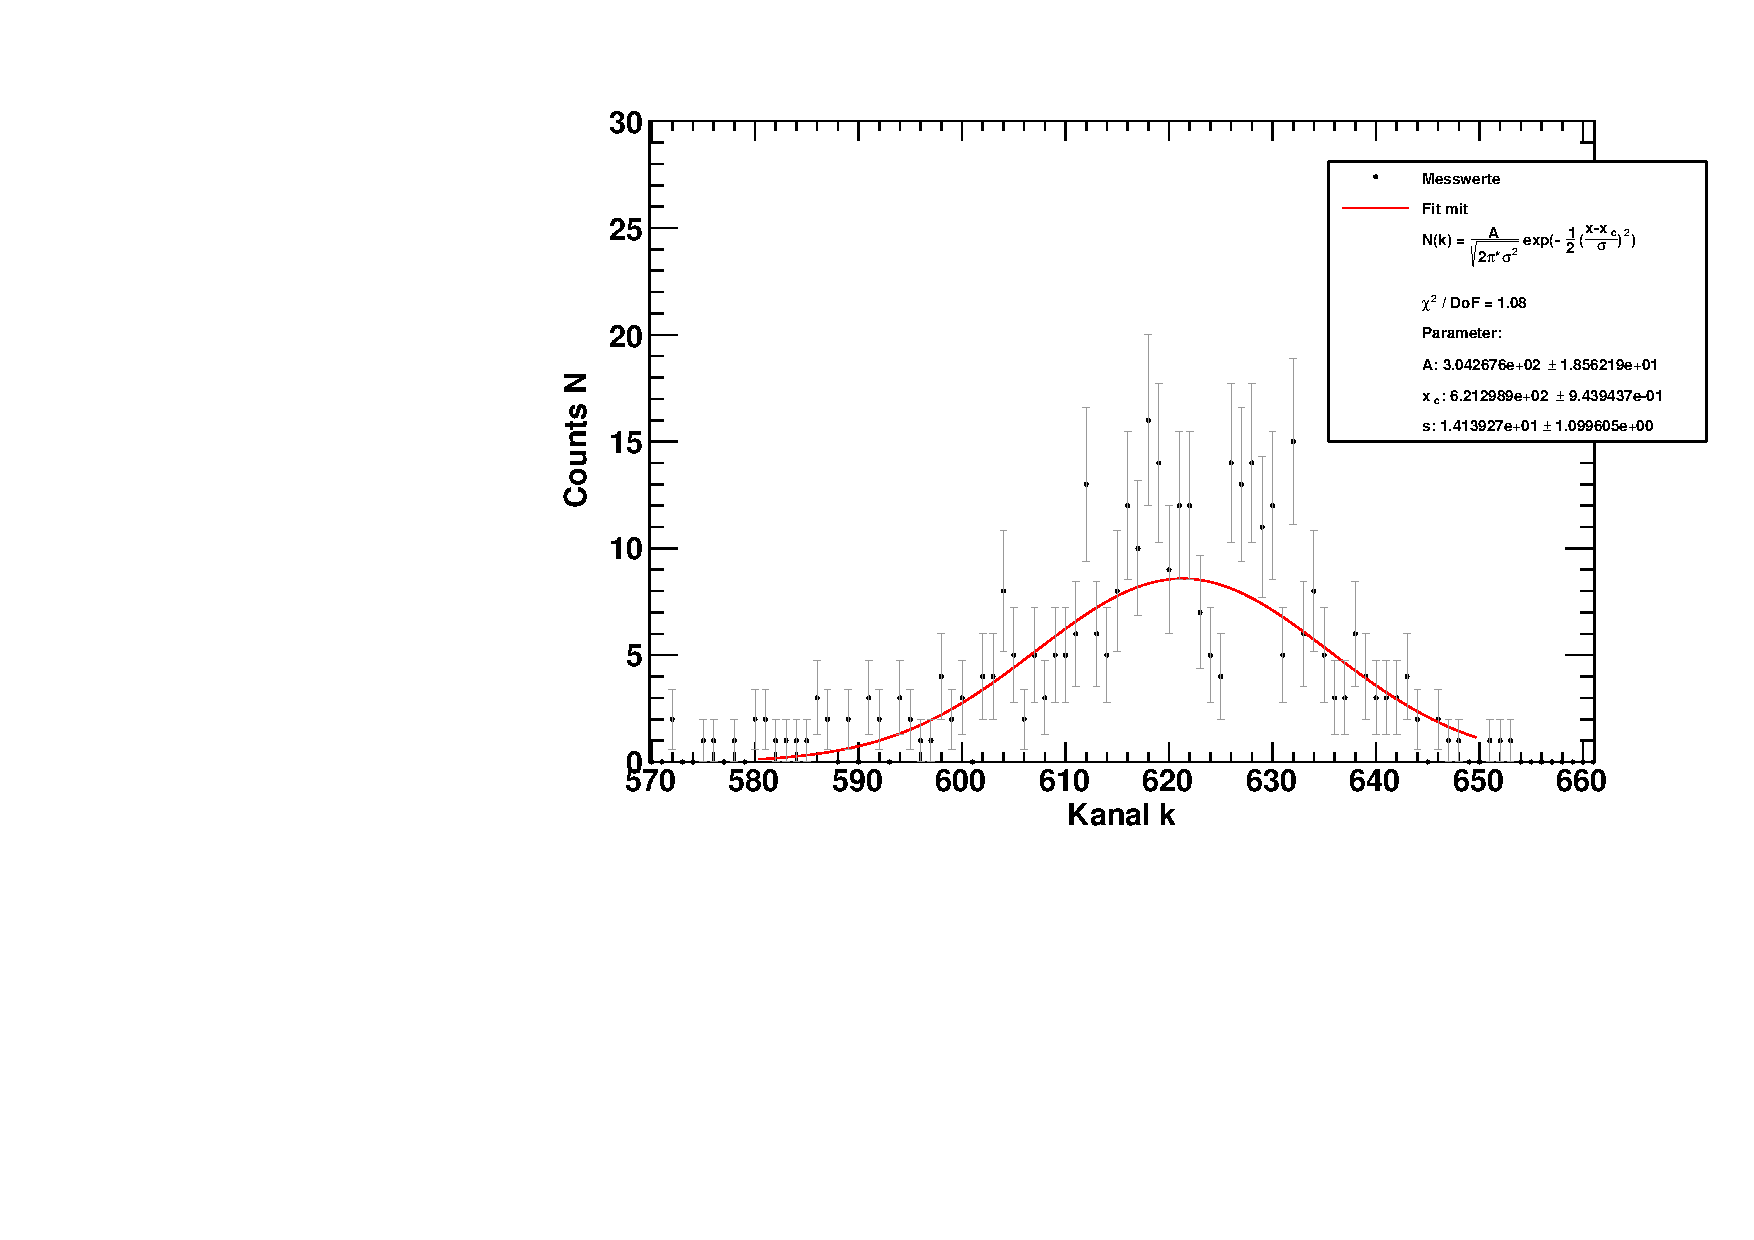
\includegraphics[width=\textwidth]{../img/part3/Co-Si_00.pdf}
  \caption{122.06\,keV-Peak von \co, gemessen mit dem Si-Detektor.}
  \label{img:co:si:peak0}
\end{center}
\end{figure}

\begin{figure}[H]
\begin{center}
  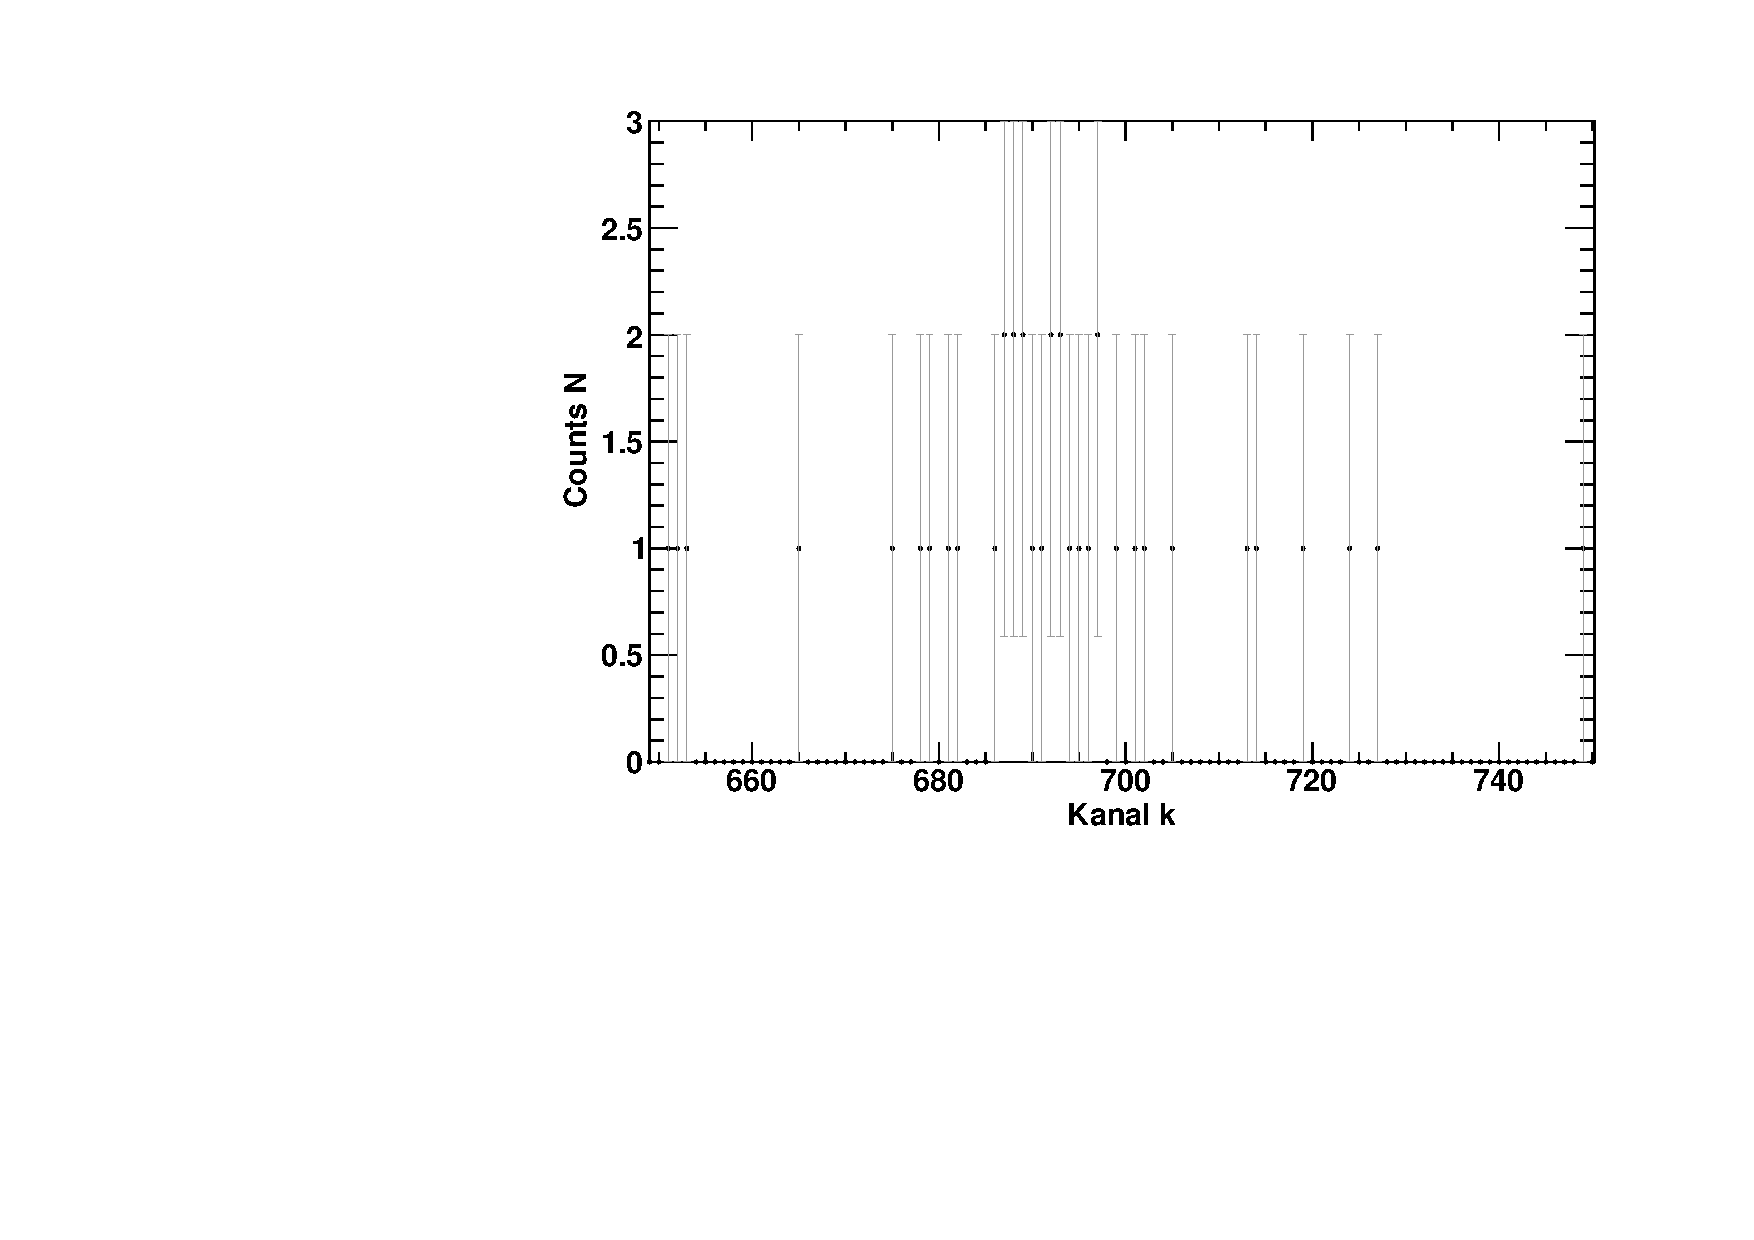
\includegraphics[width=\textwidth]{../img/part3/Co-Si_01.pdf}
  \caption{136.47\,keV-Peak von \co, gemessen mit dem Si-Detektor.}
  \label{img:co:si:peak1}
\end{center}
\end{figure}

\paragraph{Bestimmung des 136.47\,keV-Peak von \co}
Um doch noch den 136.47\,keV-Peak von \co\ fitten zu können wird jeweils von 5 Kanälen der Mittelwert der Kanäle und der Counts gebildet. 
Die Fehler werden mit Gauß'scher Fehlerfortpflanzung berechnet.
Das so erhaltene Spektrum zeigt einen klar erkennbaren Peak, der sich auch fitten lässt (\autoref{img:co:si:peak1:merged}).
\begin{figure}[H]
\begin{center}
  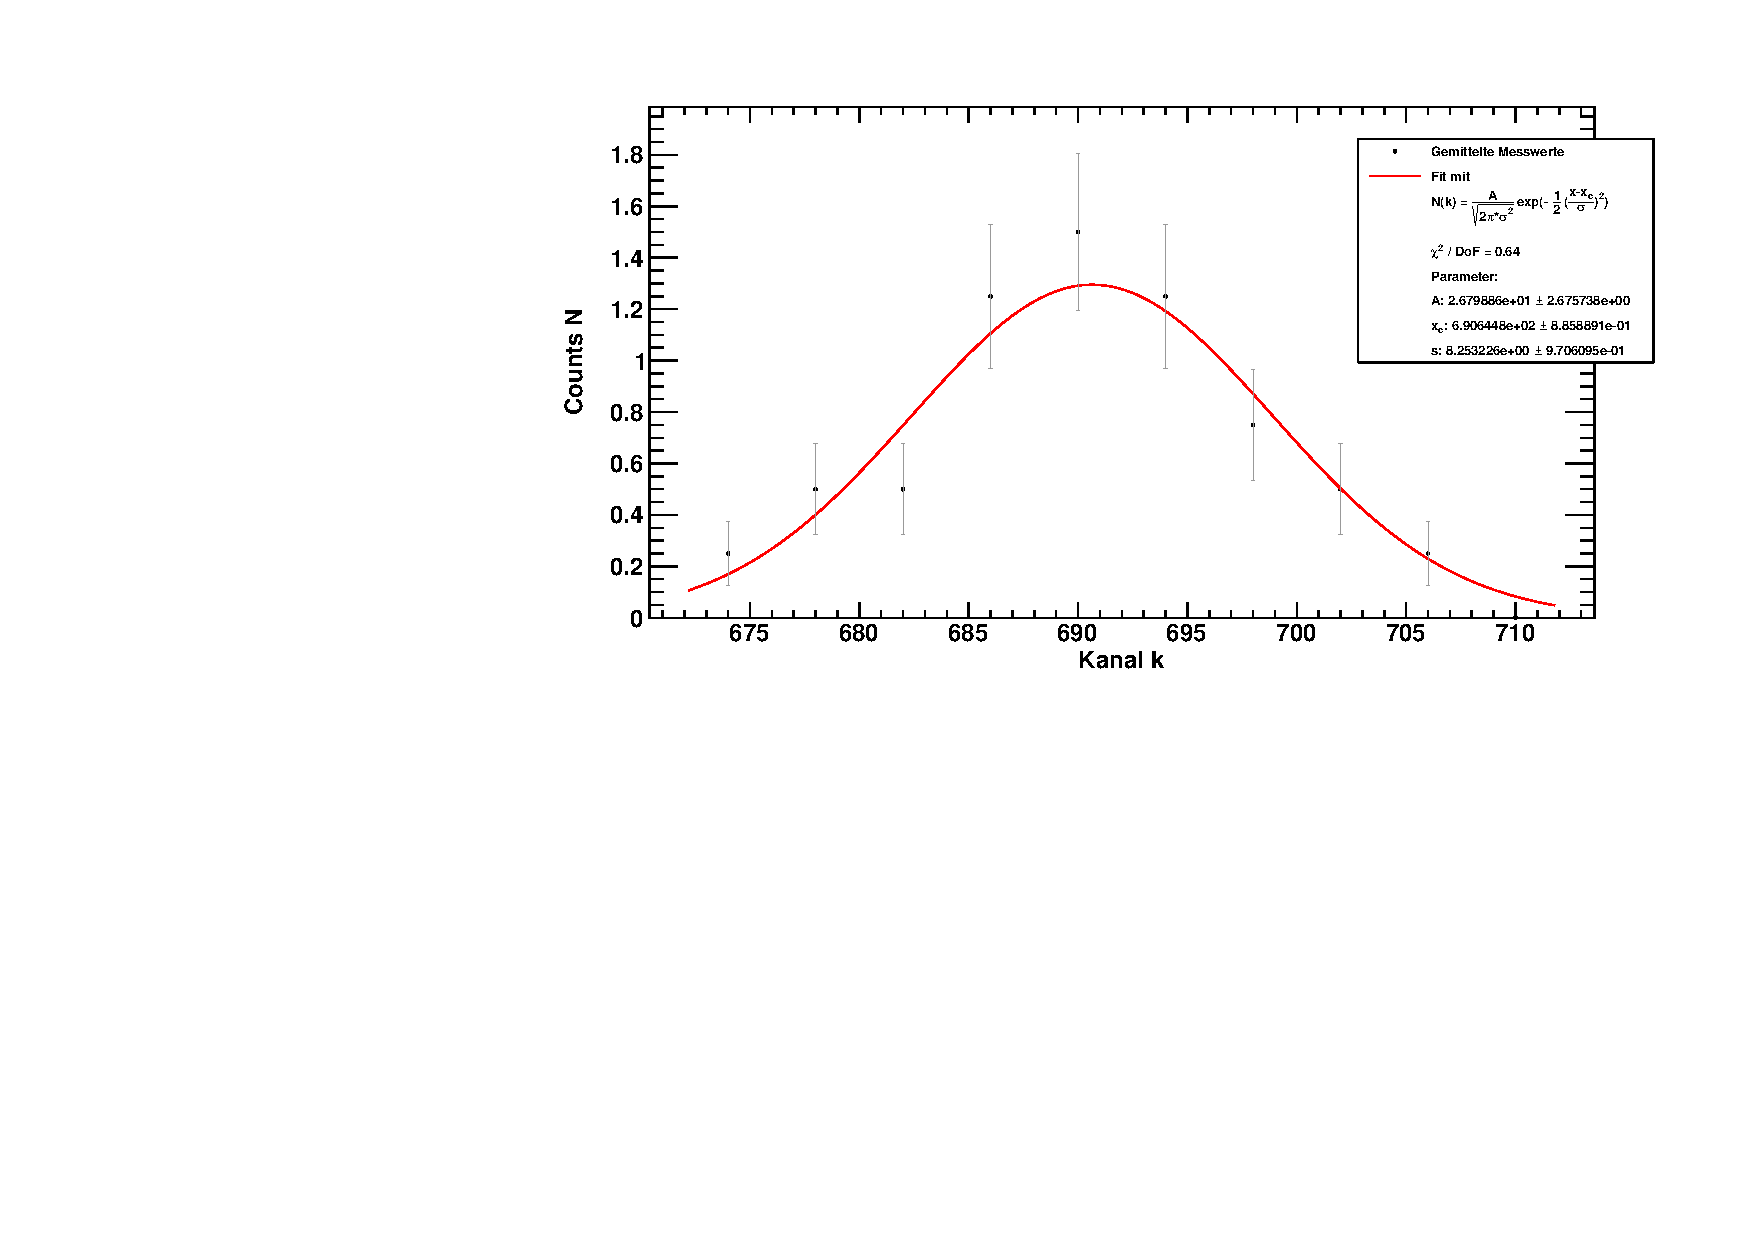
\includegraphics[width=\textwidth]{../img/part3/Co-Si_01_mergedbins.pdf}
  \caption{136.47\,keV-Peak von \co, gemessen mit dem Si-Detektor. Jeweils 5 Kanäle wurden zusammengefasst.}
  \label{img:co:si:peak1:merged}
\end{center}
\end{figure}

\paragraph{Energieeichung}
Die Energieeichung des Si-Detektors erfolgt analog zu derjenigen des CdTe-Detektors.
\begin{equation}
    E(k) = a + b\cdot k
\end{equation}
\begin{figure}[H]
\begin{center}
  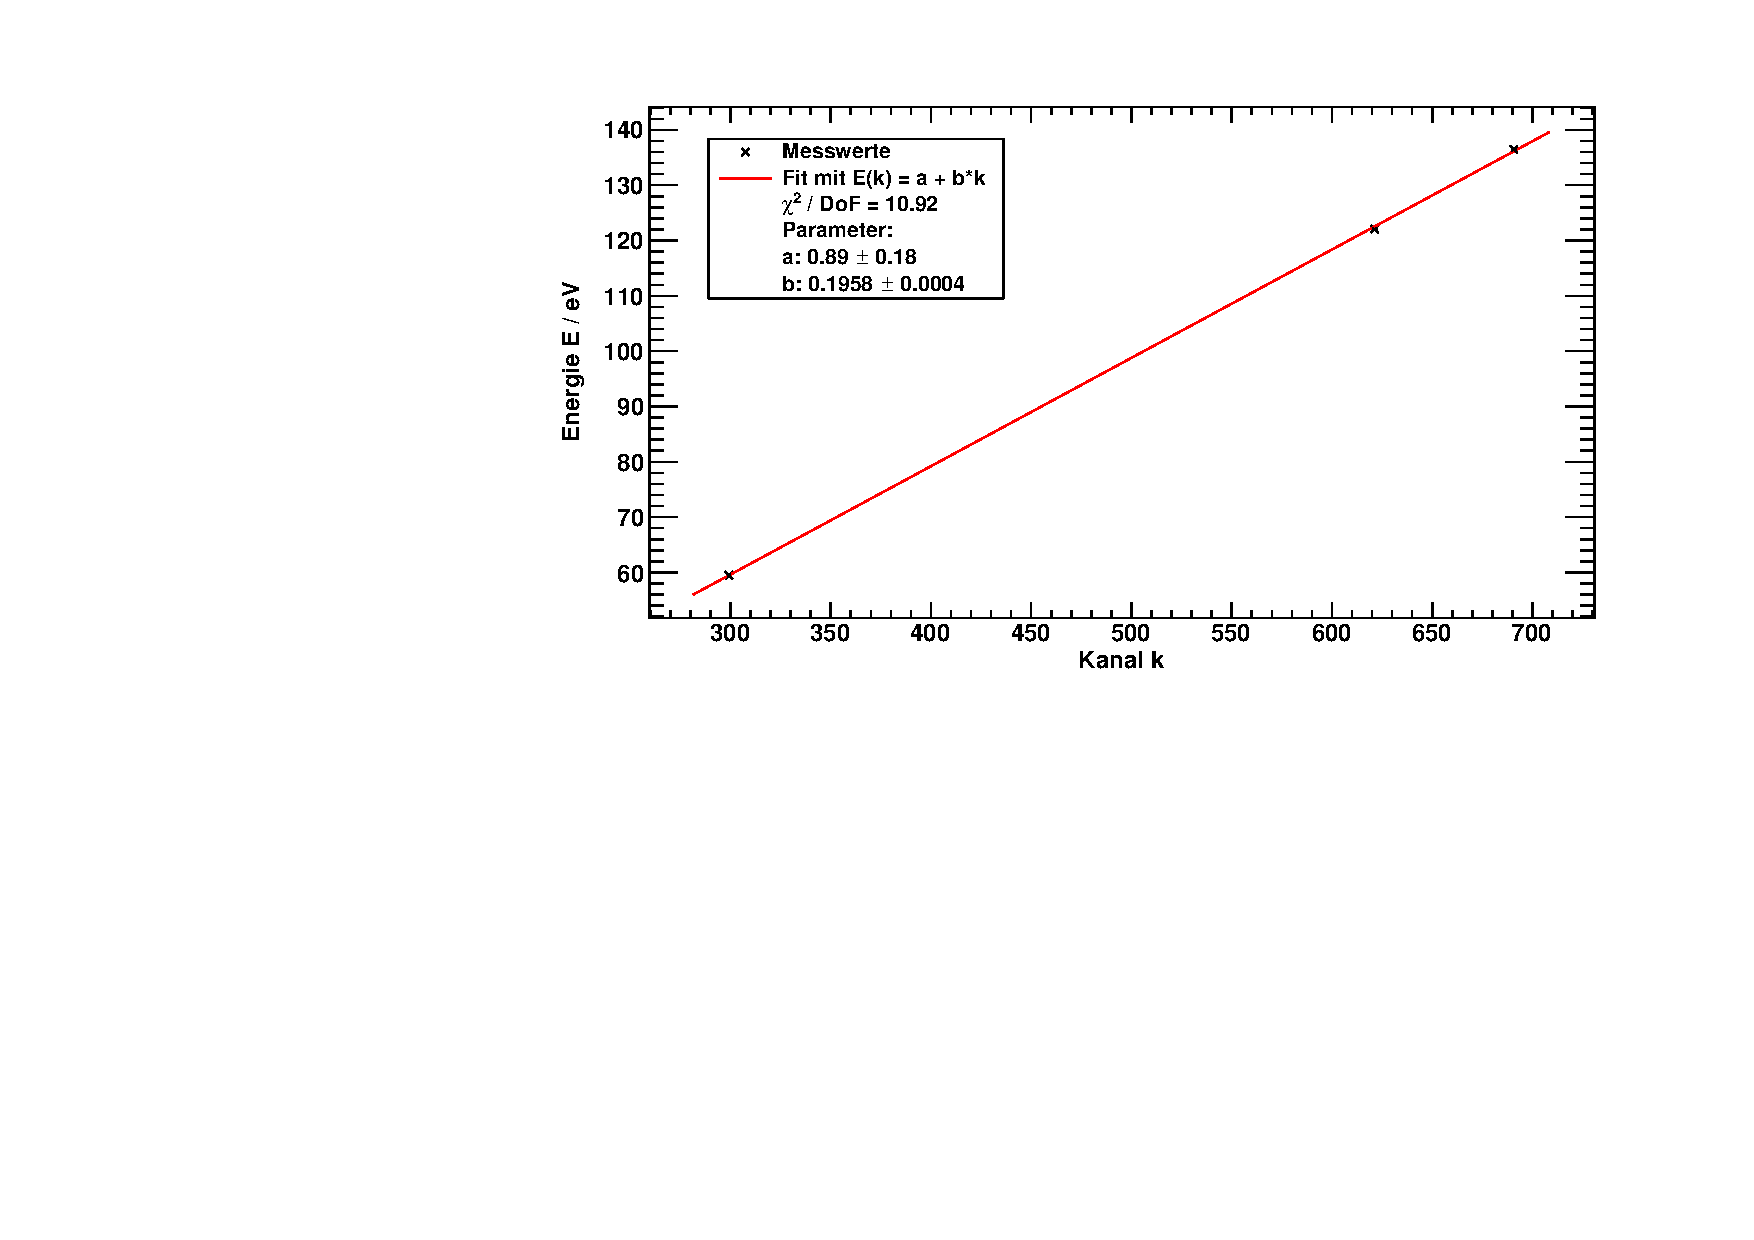
\includegraphics[width=\textwidth]{../img/part3/energygauge_Si.pdf}
  \caption{Energieeichung des Si-Detektors.}
  \label{img:si:energygauge}
\end{center}
\end{figure}
Es folgt für die Paramter:
\begin{equation}
\begin{split}
  a &= (0.89 \pm 0.18)\,\text{eV} \\
  b &= (0.1958 \pm 0.0004)\,\text{eV}
\end{split}
\end{equation}
Sie haben einen ähnlichen Wert wie die des CdTe-Detektors. 
Das $\chi^2$ ist hier ebenfalls aus den oben beschriebenen Gründen erhöht.

\paragraph{Relative Energieauflösung}
Die relative Energieauflösung des Si-Detektors wird mit \autoref{eq:rer} für jeden Peak bestimmt (\autoref{tab:si:rer}), 
die Parameter folgen aus den Fits.
\begin{table}[H]
\begin{center}
\begin{tabular}{|c|c|}
\hline 
Kanal & RER \\ \hline
299.2 $\pm$ 0.4 & 0.096 $\pm$ 0.003 \\ \hline
621.3 $\pm$ 0.9 & 0.054 $\pm$ 0.004 \\ \hline
690.6 $\pm$ 0.9 & 0.028 $\pm$ 0.003 \\ \hline
\end{tabular}
\caption{Energieauflösungen des Si-Detektors.}
\label{tab:si:rer}
\end{center}
\end{table}

\subsubsection{Absorptionsverhältnisse}
Die Absorptionswahrscheinlichkeit lässt sich mit der Amplitude $A$ aus dem Gauß-Fit und der Detektoroberfläche $a$ bestimmen: 
\begin{equation}
  \text{Abs} = \frac{A}{a}
\end{equation}
Der Quotient aus der Absorptionswahrscheinlichkeit der beiden Detektoren bei gleicher Energie liefert das Absorptionsverhältnis 
(\autoref{tab:absrel}).
\begin{table}[H]
\begin{center}
\begin{tabular}{|c|c|c|}
\hline 
Energie & $\text{Abs}_{\text{Si}} / \text{Abs}_{\text{CdTe}}$ & Literaturwert \cite{staatsex} \\ \hline
59.5 & 0.0181    $\pm$ 0.0006 & 0.0140 \\ \hline
122.06 & 0.0087 $\pm$ 0.0007 & 0.0183 \\ \hline
136.47 & 0.0090 $\pm$ 0.0010 & 0.0200 \\ \hline
\end{tabular}
\caption{Absorptionsverhältnisse von Si- und CdTe-Detektor.}
\label{tab:absrel}
\end{center}
\end{table}
Die berechneten Werte stimmen nicht mit den Literaturwerten \cite{staatsex} überein. Dies kann mehrerer Gründe haben 
(beschrieben in \cite{staatsex}), wie zum Beispiel Absorption der Epoxid- und $\text{SiO}_2$-Schicht oder Ladungsrekombination. Jedoch 
stimmt die Vorrausage von \cite{staatsex}, dass die gemessenen Werte etwa um den Faktor 2 von den Literaturwerten abweichen, für die beiden Peaks 
mit höherer Energie.


\appendix
\section{Anhang}
\subsection{Messprotokoll}
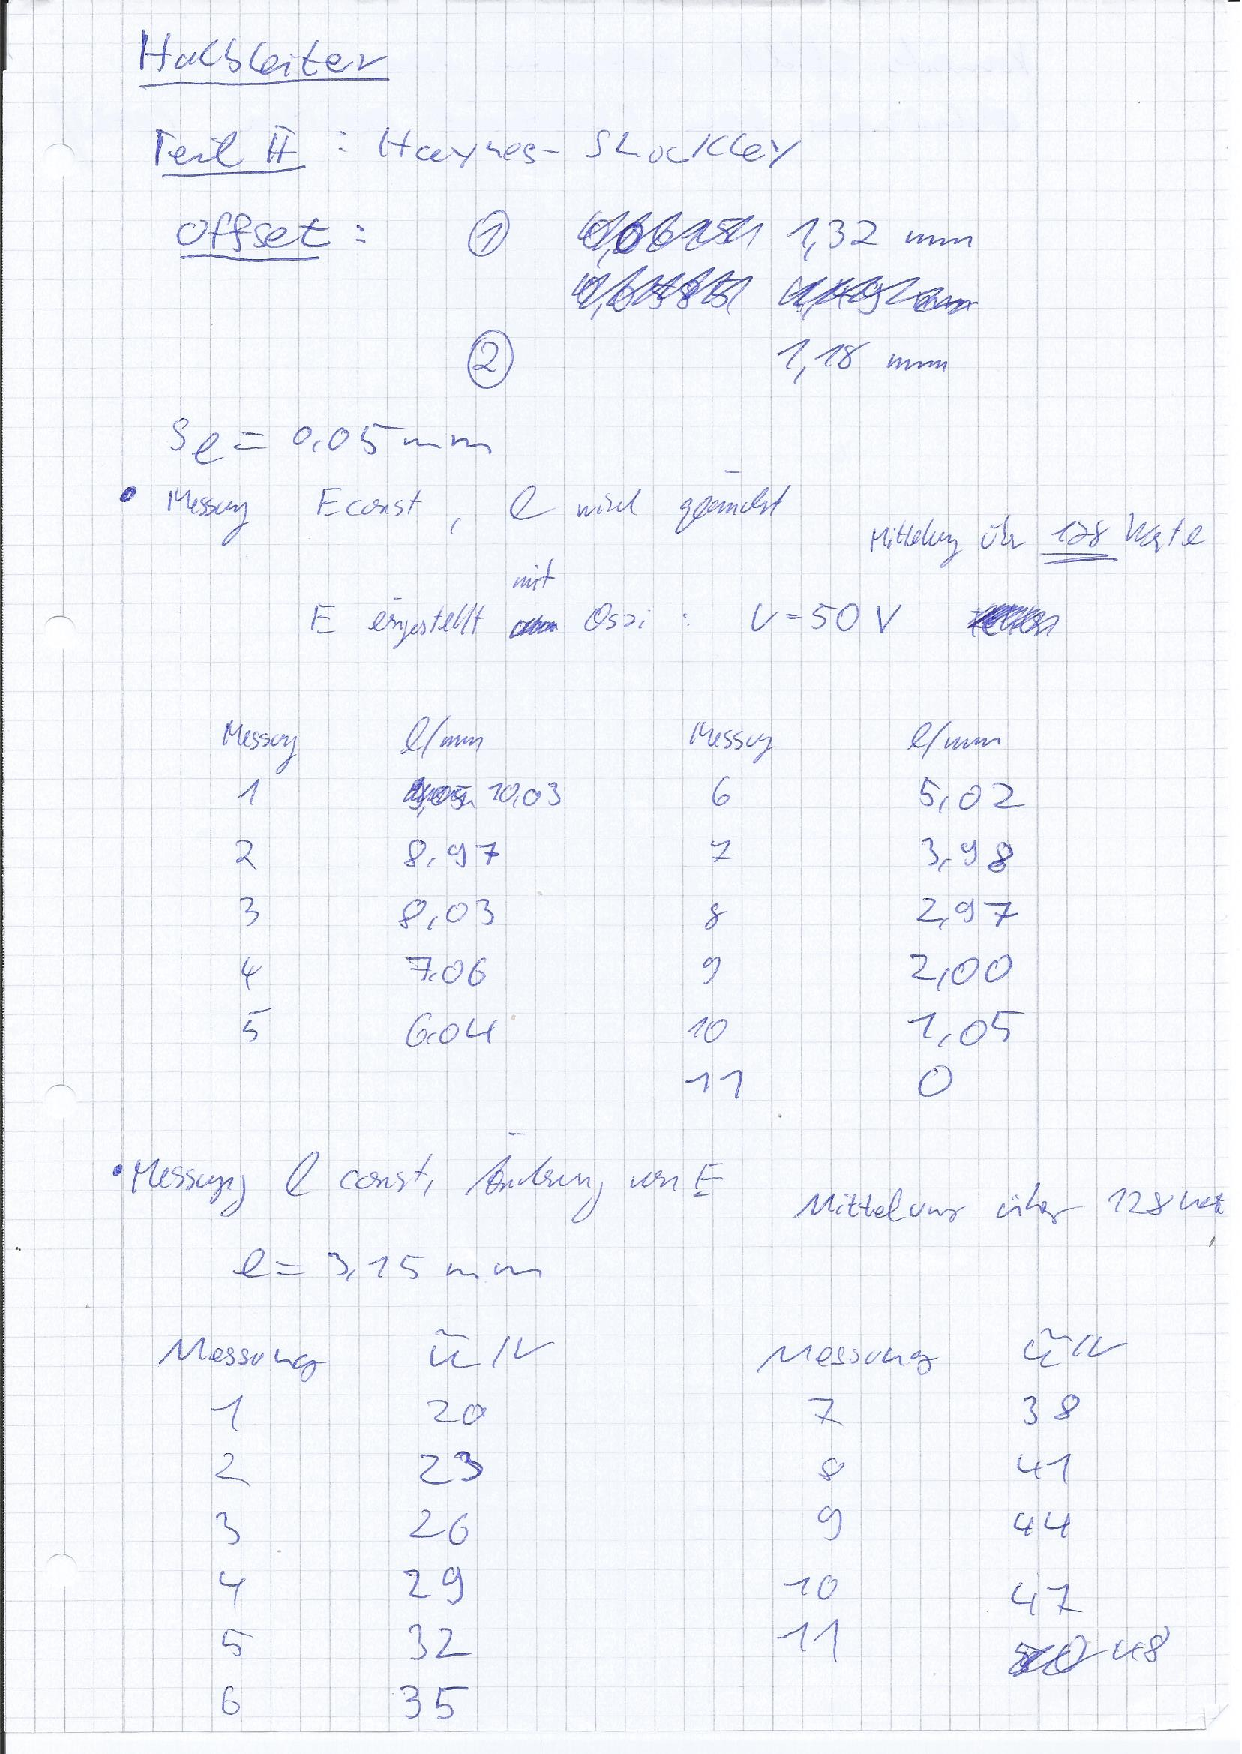
\includepdf[pages={-}]{../data/protocol.pdf}


\end{document}